\documentclass[12pt,english,french,twoside]{report}\usepackage[]{graphicx}\usepackage[]{color}
%% maxwidth is the original width if it is less than linewidth
%% otherwise use linewidth (to make sure the graphics do not exceed the margin)
\makeatletter
\def\maxwidth{ %
  \ifdim\Gin@nat@width>\linewidth
    \linewidth
  \else
    \Gin@nat@width
  \fi
}
\makeatother

\definecolor{fgcolor}{rgb}{0.345, 0.345, 0.345}
\newcommand{\hlnum}[1]{\textcolor[rgb]{0.686,0.059,0.569}{#1}}%
\newcommand{\hlstr}[1]{\textcolor[rgb]{0.192,0.494,0.8}{#1}}%
\newcommand{\hlcom}[1]{\textcolor[rgb]{0.678,0.584,0.686}{\textit{#1}}}%
\newcommand{\hlopt}[1]{\textcolor[rgb]{0,0,0}{#1}}%
\newcommand{\hlstd}[1]{\textcolor[rgb]{0.345,0.345,0.345}{#1}}%
\newcommand{\hlkwa}[1]{\textcolor[rgb]{0.161,0.373,0.58}{\textbf{#1}}}%
\newcommand{\hlkwb}[1]{\textcolor[rgb]{0.69,0.353,0.396}{#1}}%
\newcommand{\hlkwc}[1]{\textcolor[rgb]{0.333,0.667,0.333}{#1}}%
\newcommand{\hlkwd}[1]{\textcolor[rgb]{0.737,0.353,0.396}{\textbf{#1}}}%

\usepackage{framed}
\makeatletter
\newenvironment{kframe}{%
 \def\at@end@of@kframe{}%
 \ifinner\ifhmode%
  \def\at@end@of@kframe{\end{minipage}}%
  \begin{minipage}{\columnwidth}%
 \fi\fi%
 \def\FrameCommand##1{\hskip\@totalleftmargin \hskip-\fboxsep
 \colorbox{shadecolor}{##1}\hskip-\fboxsep
     % There is no \\@totalrightmargin, so:
     \hskip-\linewidth \hskip-\@totalleftmargin \hskip\columnwidth}%
 \MakeFramed {\advance\hsize-\width
   \@totalleftmargin\z@ \linewidth\hsize
   \@setminipage}}%
 {\par\unskip\endMakeFramed%
 \at@end@of@kframe}
\makeatother

\definecolor{shadecolor}{rgb}{.97, .97, .97}
\definecolor{messagecolor}{rgb}{0, 0, 0}
\definecolor{warningcolor}{rgb}{1, 0, 1}
\definecolor{errorcolor}{rgb}{1, 0, 0}
\newenvironment{knitrout}{}{} % an empty environment to be redefined in TeX

\usepackage{alltt}
\usepackage[francais]{babel}
\usepackage[T1]{fontenc}
\usepackage{lmodern}
\usepackage[utf8]{inputenc}
% inclu un fichier de bibliothèques
\include{rpu-2012.sty}

% la directive suivante permet d'utiliser le séparateur de milliers. 
%Deux formulation sont utilisables mais exclusives l'une de l'autre. L'instruction "autolanguage" permet d'utiliser \nombre{} ou \np{}
% exemple: L'ensemble des SU ont déclaré \np{length(e)} passages en 2013
%\usepackage{numprint}
\usepackage[autolanguage,np]{numprint}

% la ligne qui suit donne un titre interne au document pdf et crée des liens cliquables en bleu sur les tables et figures
\usepackage[pdftitle={RPU2012-Resural}, colorlinks=true, linkcolor=blue,citecolor=blue, urlcolor=blue, linktocpage=true, breaklinks=true]{hyperref}

\usepackage[left=4cm,right=3cm,top=2cm,bottom=2cm]{geometry}
\usepackage{graphicx}

\usepackage{amsmath}
\usepackage{amsfonts}
\usepackage{amssymb}
\usepackage{xcolor} 
\usepackage{hyperref} 
\usepackage{tikz} 
% Mise en page
% LE zone gauche page paire
% CE zone médiane page paire
% RE zone droite page paire
% LO zone gauche page impaire
% CO zone médiane page impaire
% RO zone droite page impaire
% fancyhead gère le haut de page
% fancyfoot gère le bas de page
\usepackage{fancyhdr}
\pagestyle{fancy}
\fancyhead[LE,CE,RE,LO,CO,RO]{}
\fancyhead[LE,RO]{\scshape\thepage}
\fancyhead[CE]{\scshape\leftmark}
\fancyhead[CO]{\scshape\rightmark}

\fancyfoot[CE]{Document de travail - non validé}
\fancyfoot[CO]{Document de travail - non validé}

\usepackage{fancyvrb}

\usepackage{longtable}

\usepackage{makeidx}
\makeindex

\bibliographystyle{plain}

\makeglossary
%\makeindex -s glossaire.ist RPU2013.glo -o RPU2013.glx

% \newenvironment{leglossaire}{\begin{list}{}{%
%   \setlength{\labelwidth}{.5\textwidth}%
%   \setlength{\labelsep}{-.8\labelwidth}%
%   \setlength{\itemindent}{\parindent}%
%   \setlength{\leftmargin}{25pt}%
%   \setlength{\rightmargin}{0pt}%
%   \setlength{\itemsep}{.8\baselineskip}%
%   \renewcommand{\makelabel}[1]{\boiteentreeglossaire{##1}}}}
% {\end{list}}
%       
% \newcommand{boiteentreeglossaire}[1]{%
%   \parbox[b]{\labelwidth}{%
%   \setlength{\fboxsep}{3pt}%
%   \setlength{\fboxrule}{.4pt}%
%   \shadow{\sffamily#1}\\\hfill\mbox{}}}

% Définitions de constantes


\IfFileExists{upquote.sty}{\usepackage{upquote}}{}


\begin{document}

\title{Analyse des données RPU 2013 de la région Alsace}
\author{RESURAL\thanks{Réseau des urgences en Alsace - Equipe de coordination Dr J.C.
Bartier \& Madame Christine Hecker}}
\date{\today}
\maketitle

%\SweaveOpts{concordance=TRUE}
%\SweaveOpts{fig.path='./figure/rpu2013-', comment=NA, prompt=FALSE}

\newpage

\begin{itemize}\raggedright
  \item R version 2.15.1 (2012-06-22), \verb|x86_64-pc-linux-gnu|
  \item Locale: \verb|LC_CTYPE=fr_FR.UTF-8|, \verb|LC_NUMERIC=C|, \verb|LC_TIME=fr_FR.UTF-8|, \verb|LC_COLLATE=fr_FR.UTF-8|, \verb|LC_MONETARY=fr_FR.UTF-8|, \verb|LC_MESSAGES=fr_FR.UTF-8|, \verb|LC_PAPER=C|, \verb|LC_NAME=C|, \verb|LC_ADDRESS=C|, \verb|LC_TELEPHONE=C|, \verb|LC_MEASUREMENT=fr_FR.UTF-8|, \verb|LC_IDENTIFICATION=C|
  \item Base packages: base, datasets, graphics, grDevices,
    methods, stats, utils
  \item Other packages: knitr~1.4.1
  \item Loaded via a namespace (and not attached): digest~0.6.3,
    evaluate~0.4.7, formatR~0.9, stringr~0.6.2, tools~2.15.1
\end{itemize}



\tableofcontents
\listoftables
\listoffigures



%======================================================== PARTIE 1
\part{Le Réseau des urgences en Alsace}

\chapter{Historique}

% historique.Rnw

Le Réseau des Urgences en Alsace a été créé en août 2008 sous forme d'une association de droit local dans la foulée de la circulaire de 2007.

\index{RESURAL!historique}


\chapter{Organisation géographique}

% geographie.Rnw

L'Alsace est la plus petite région de France (n°42) avec la Corse. Elle est formée de deux départements, le bas-Rhin (67) et le haut-Rhin (68), dont les chef-lieu sont respectivement Strasbourg et Colmar.La préfecture régionale siège à Strasbourg comme l'agence régionale de l'hospitalisation \index{ARS} (ARS).

La région est divisée en quatre secteurs sanitaires er douze tritoires de proximité.

\section{Les secteurs sanitaires}
\index{Alsace!secteurs sanitaires}
\index{Secteurs sanitaires}

L'alsace est divisée en quatre secteurs sanitaires
\begin{enumerate}
  \item secteur 1: Haguenau, Wissembourg et Saverne
  \item secteur 2: Strasbourg
  \item secteur 3: Sélestat et Colmar. C'est un territoire qui est à cheval sur les deux départements d'Alsace.
  \item secteur 4: Mulhouse
\end{enumerate}

\begin{knitrout}
\definecolor{shadecolor}{rgb}{0.969, 0.969, 0.969}\color{fgcolor}
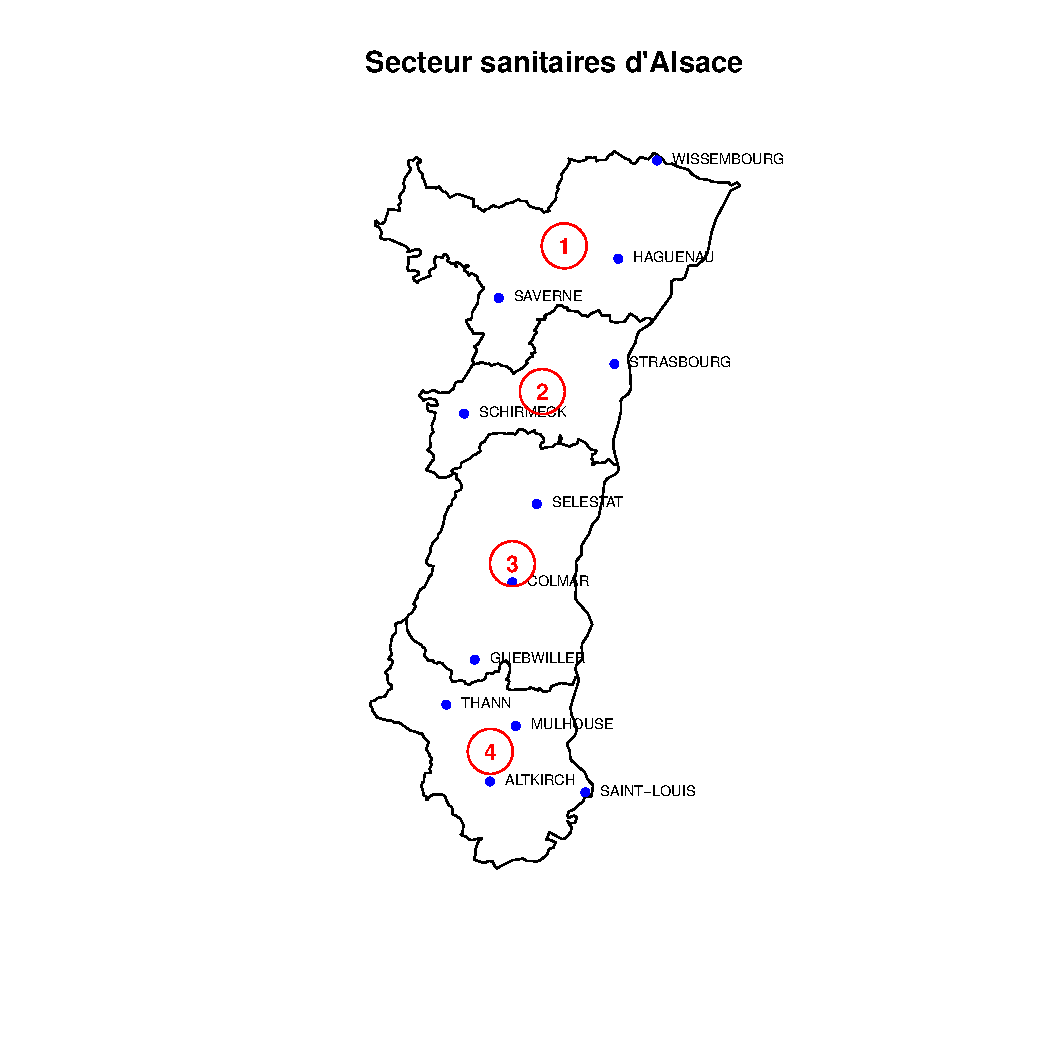
\includegraphics[width=\maxwidth]{figure/carte_secteurs_sanitaires} 

\end{knitrout}



\section{Les territoires de proximité}
\index{Alsace!territoires de proximité}
\index{Territoires de proximité}

Il existe douze territoires de proximité:
\begin{enumerate}
  \item territoire 1: Wissembourg
  \item territoire 2: Haguenau
  \item territoire 3: Saverne
  \item territoire 4: Strasbourg
  \item territoire 5: Molsheim-Schirmeck
  \item territoire 6: Sélestat-Obernai
  \item territoire 7: Colmar
  \item territoire 8: Guebwiller
  \item territoire 9: Thann
  \item territoire 10: Mulhouse
  \item territoire 11: Altkirch
  \item territoire 12: Saint-Louis
\end{enumerate}

% carte des territoires de santé
\begin{figure}[ht]
 \centering
 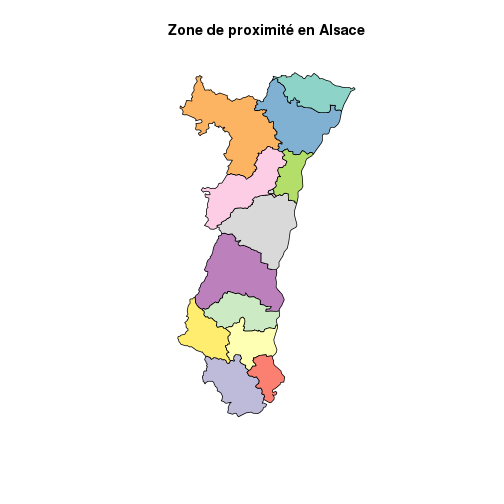
\includegraphics[height=15cm,keepaspectratio=true]{../figure/zone_proximite.png}
 % image.: 0x0 pixel, 0dpi, nanxnan cm, bb=
 \caption{L'Alsace compte 12 territoires de proximité}
 \label{fig:zp}
\end{figure}

\section{Démographie}
\subsection{Généralités}
\index{Alsace!démographie}

En France, les populations légales sont calculées par l'INSEE sur la base de définitions réglementaires à partir de recensement de la population. Ce document utilise la \emph{Population municipale} \ref{Population_municipale} \index{Population@Population!municipale}  qui est la nouvelle dénomination de la population sans double comptes. Le chiffre est donc inférieur de celui de la \emph{Population totale} qui est égale à la somme de la population municipale et de la population comptée à part d'une commune.

\subsection{Classes d'age}
Les RPU divisent l'age des patients en trois catégories:
\begin{enumerate}
  \item Les moins de un an
  \item de 1 an à 75 ans
  \item les plus de 75 ans
\end{enumerate}

Les calculs sont effectués à partir du fichier xxx de l'INSEE qui recense l'ensemble de la population par commune et par tranches de un an. La version utilisée est celle du 1er janvier 2010 (tab.\ref{pop}). Le secteur de proximité de Strasbourg qui est aussi le plus peuplé, compte le plus grand nombre de personnes de 75 ans et plus (figure \ref{fig:75ans} page \pageref{fig:75ans})

\begin{table}
\begin{center}
\begin{tabular}{|l|l|r|r|}
  \hline
  Tranche d'age & Abréviation & Effectif & Pourcentage \\
  \hline
  \hline
  Moins de 1 an & pop0 & \np{21903.14} & 1.19 \\
  De 1 à 75 ans & pop1\_75 & \np{1690073.00} & 92.00 \\
  Plus de 75 ans& pop75 & \np{125110.90} & 6.81 \\
  \hline
  Total & pop\_tot & \np{1837087.00} & 100.00 \\
  \hline
\end{tabular}
\caption{Population d'Alsace (janvier 2010)}
\label{pop}
\end{center}
\end{table}

% carte des plus de 75 ans
\begin{figure}[ht]
 \centering
 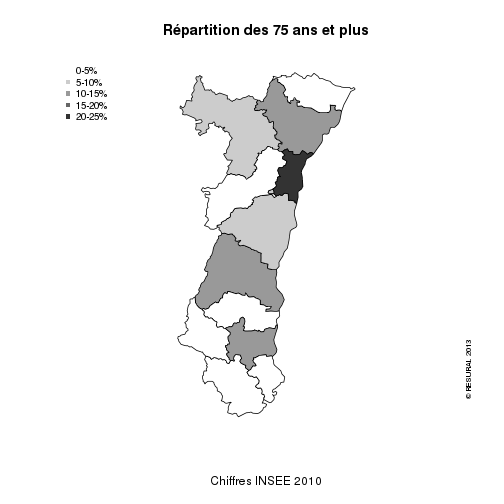
\includegraphics[height=15cm,keepaspectratio=true]{../figure/75ans.png}
 % image.: 0x0 pixel, 0dpi, nanxnan cm, bb=
 \caption[Répartition des 75 ans et plus]{Les personnes de 75 ans et plus en Alsace en fonction du territoire de proximté (en pourcentage du nombre total de 75 ans et plus).}
 \label{fig:75ans}
\end{figure}

\section{Les services d'accueil des urgences (SAU)}
\index{Services d'urgence!en Alsace}
\index{Alsace!services d'urgence}

L'Alsace compte actuellement 14 services d'urgence (SU) officiellement labellisés. On prend également en compte la clinique Saint-Luc de Schirmeck qui fait fonctionner une policlinique recevant plus de \np{8000} passages par an.

\begin{figure}[ht]
 \centering
\begin{knitrout}
\definecolor{shadecolor}{rgb}{0.969, 0.969, 0.969}\color{fgcolor}
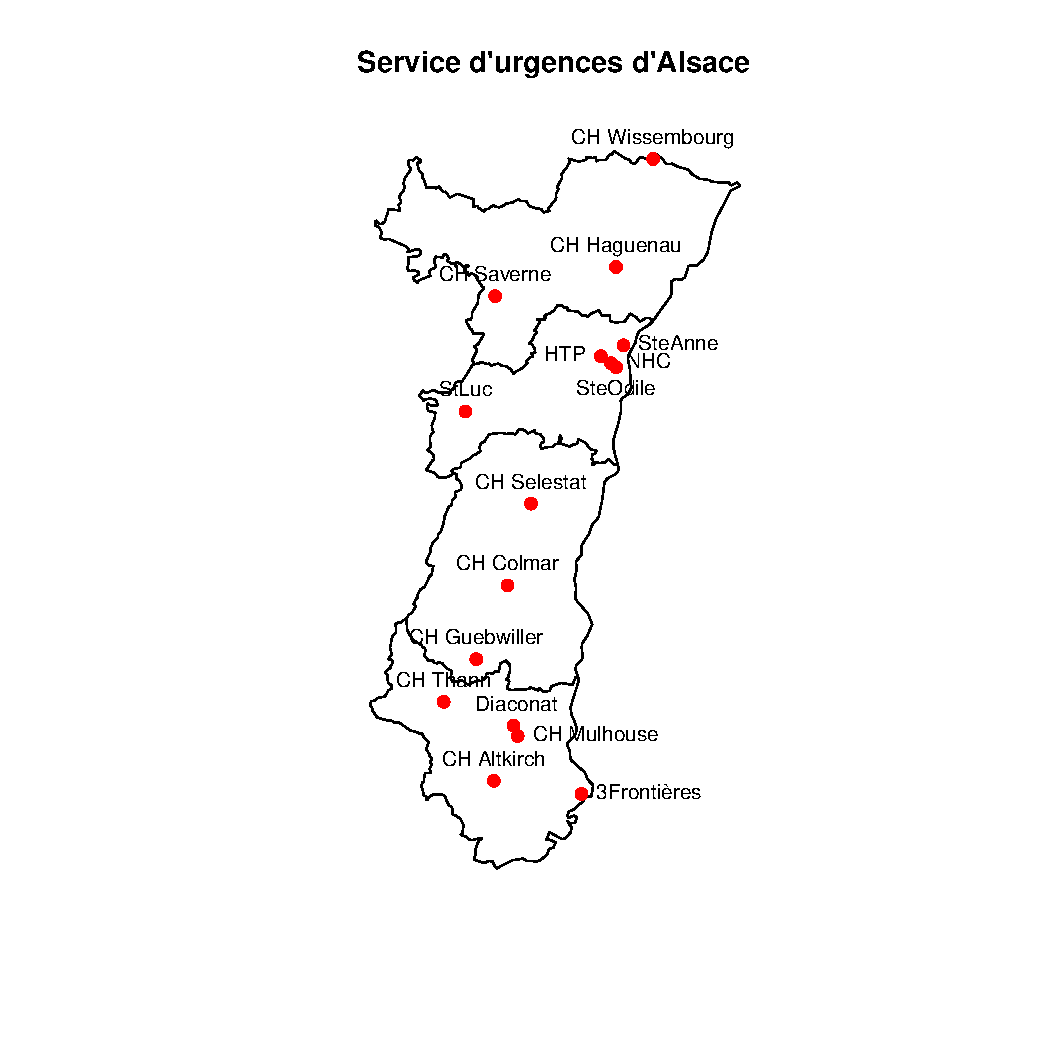
\includegraphics[width=\maxwidth]{figure/carte_sau_2} 

\end{knitrout}

 \caption[Services d'urgenced'Alsace]{L'Alsace compte 14 services d'urgence labellisés sur 15 sites.}
 \label{fig:su_alsace}
\end{figure}



\begin{table}
\begin{center}
\begin{tabular}{|c|c|c|c|l|}
  \hline
& Finess utilisé & Finess géographique & Finess Juridique & Structure \\
  \hline
  \hline
1 & 670780055 &   & 670780055 & HUS \\
2 & 670780543 & 670000272 & 670780543 & CH Wissembourg \\
3 & 670000397 & 670000397  & 670780691 & CH Selestat \\
4 & 670780337 & 670000157 & 670780337 & CH Haguenau \\
5 &   & 670000165 & 670780345 & CH Saverne \\
6 & 670016237  & 670016237  & 670016211 & Clinique ste Odile \\
7 &   & 670780212 & 670014604 & Clinique Ste Anne \\
8 & 680000973 & 680000684 & 680000973 & CH Colmar \\
9 & 680000197  & 680000197  & 680000049 & Clinique des trois frontières \\
10 & 680000486 & 680000544  & 680000395 & CH Altkirch \\
11 & 680000700 & 680000700 & 680001005 & CH Guebwiller \\
12 & 680000627 & 680000627 & 680000486 & CH Mulhouse FG \\
13 &   & 680000601 & 680000437 & CH Thann \\
14 &   & 680000320  & 680000643 & Diaconat-Fonderie (St Sauveur) \\
\hline
\end{tabular}
\caption{Service d'accueil des urgences d'Alsace}
\label{summary}
\end{center}
\end{table}

\chapter{Les acteurs}

% acteurs.Rnw

% penser au secteur libéral

\section{Exhaustivité quantitative}



Les données proviennent des RPU produits par les hôpitaux d'Alsace ayant l'autorisation de faire fonctionner un service d'urgence (SU). La liste des structures hospitalières ayant fournit des informations alimentant le présent rapport est fournie par la table \ref{tab1}, page \pageref{tab1}.

Tous ces hôpitaux fournissent des données depuis le premier janvier 2013 sauf le CH Saverne qui a commencé en Juillet 2013.

Deux structures ne fournissent pas encore de RPU. Il s'agit de la clinique Sainte-Anne à Strasbourg (Groupe hospitalier Saint-Vincent) et du Centre Hospitalier de Thann.

Certaines données peuvent être recoupées avec celles du serveur régional mis en place en 2006 par l'ARS: 

\fbox{Voir SAU2013}

% latex table generated in R 2.15.1 by xtable 1.7-1 package
% Wed Sep 18 09:03:24 2013
\begin{table}[ht]
\centering
\begin{tabular}{|l|r|r|l|r|}
  \hline
 & n & \% & Hôpitaux & Date d'inclusion \\ 
  \hline
3Fr & 10752 & 4.84 & Clinique des 3 frontières & 01/01/2013 \\ 
  Alk & 4552 & 2.05 & CH Altkirch & 01/04/2013 \\ 
  Col & 44271 & 19.91 & CH Colmar & 01/01/2013 \\ 
  Dia & 19699 & 8.86 & Diaconat Fonderie & 01/01/2013 \\ 
  Geb & 10207 & 4.59 & CH Guebwiller & 01/01/2013 \\ 
  Hag & 23542 & 10.59 & CH Haguenau & 01/01/2013 \\ 
  Hus & 25498 & 11.47 & Hôpitaux Universitaires de Strasbourg & 01/01/2013 \\ 
  Mul & 36619 & 16.47 & CH Mulhouse & 07/01/2013 \\ 
  Odi & 17327 & 7.79 & Clinique Ste Odile & 01/01/2013 \\ 
  Sel & 18502 & 8.32 & CH Sélestat & 01/01/2013 \\ 
  Wis & 8521 & 3.83 & CH Wissembourg & 01/01/2013 \\ 
  Sav & 2861 & 1.29 & CH Saverne & 23/07/2013 \\ 
   \hline
\end{tabular}
\caption{Structures hospitalières participantes en 2013} 
\label{tab1}
\end{table}



\section{Exhaustivité qualitative}

Les informations de nature administrative (code postal, commune d'origine, sexe, date de naissance,\dots ) sont correctement renseignées avec une exhaustivité de $100\%$.

Les données à caractère plus médical comme le motif de consultation ou le diagnostic principal ont une exhaustivité moins bonne, de l'ordre de $70\%$.

% latex table generated in R 2.15.1 by xtable 1.7-1 package
% Wed Sep 18 09:03:27 2013
\begin{table}[ht]
\centering
\begin{tabular}{|l|r|}
  \hline
 & \% \\ 
  \hline
id & 0.00 \\ 
  CODE\_POSTAL & 0.00 \\ 
  COMMUNE & 0.00 \\ 
  ENTREE & 0.00 \\ 
  EXTRACT & 0.00 \\ 
  FINESS & 0.00 \\ 
  NAISSANCE & 0.00 \\ 
  SEXE & 0.00 \\ 
  AGE & 0.00 \\ 
  SORTIE & 9.30 \\ 
  MODE\_ENTREE & 10.72 \\ 
  GRAVITE & 13.66 \\ 
  MODE\_SORTIE & 14.81 \\ 
  TRANSPORT & 21.16 \\ 
  TRANSPORT\_PEC & 24.94 \\ 
  DP & 31.83 \\ 
  PROVENANCE & 34.07 \\ 
  MOTIF & 35.81 \\ 
  DESTINATION & 78.90 \\ 
  ORIENTATION & 80.01 \\ 
   \hline
\end{tabular}
\caption{Données manquantes en 2013} 
\label{tab2}
\end{table}




Les informations sont résumées dans la table \ref{tab2}, page \pageref{tab2}.

\chapter{RESURAL}

% resural.Rnw
\index{RESURAL}

Le réseau des urgences en Alsace (RESURAL) est une association à but non lucratif, de droit local Alsace-Moselle, dont les statuts sont déposés au tribunal de Strasbourg. Le réseau a été fondé en août 2008. En son membre de droit les services d'urgence intra et extra-hospitaliers, adultes et pédiatriques, possédant une autorisation d'exercer cette spécialité, délivrée par l'agence régionale de santé (ARS). \index{ARS}

Elle est domiciliée aux Hôpitaux Universitaires de Strasbourg.

Elle est dirigée par un conseil d'administration et représentée par son preésident, le Docteur Bruno Goulesque.

Son fonctionnement est assuré par une équipe de coordination, composée d'un médecin coordinateur à mi-temps et d'une assistante à mi-temps. Cette équipe est opérationnelle depuis le 1er février 2013.

\chapter{L'observatoire des urgences en Alsace (ORUDAL)}

% orudal.Rnw

L'observatoire des urgences en Alsace (ORUDAL) est une structure informelle animée par le réseau des urgences en Alsace.
\index{ORUDAL}
\index{Observatoire des urgences en Alsace}

Il est composé des organismes suivants:
\begin{enumerate}
  \item RESURAL \index{RESURAL}
  \item ARS Alsace
  \item CIRE-InVS
  \item Alsace e-santé
  \item CMUNE
\end{enumerate}


\section*{Les partenaires}

  \subsection*{Agence Régionale de Santé}
    \index{ARS}
    
  \subsection*{Alsace e-santé}
    \index{Alsace e-santé}
    
  \subsection*{CIRE-INVS}
    \index{CIRE-INVS}
    
  \subsection*{Collège de médecine d'urgence (CMUNE)}
    \index{CMUNE}

\section*{FEDORU}
  \index{FEDORU}
  
La fédération des observatoires des urgences et structures apparentés a été crée en octobre 2013 à l'initiative de quelques organisme régionaux dont Résural sur une proposition de l'ORUPACA \index{ORUPACA}

  
\chapter{Le Résumé du passage aux urgences}

% rpu.Rnw

\section*{RPU}

Les Résumés de Passage aux Urgences (RPU) ont été transmis par le Centre Hospitalier de Sélestat à partir de 2008. 
La table \emph{rpu} du serveur de test comporte 

{\ttfamily\noindent\bfseries\color{errorcolor}{\\Error in nrow(d2) : objet 'd2' introuvable}} lignes et 

{\ttfamily\noindent\bfseries\color{errorcolor}{\\Error in ncol(d2) : objet 'd2' introuvable}} colonnes. La période érudiée couvre toute l'année 2009 s'étend (du 

{\ttfamily\noindent\bfseries\color{errorcolor}{\\Error in eval(expr, envir, enclos) : objet 'd2' introuvable}} au 

{\ttfamily\noindent\bfseries\color{errorcolor}{\\Error in eval(expr, envir, enclos) : objet 'd2' introuvable}}), ce qui correspond à toutes les entrées de cette année. Les RPU sont saisis selon la version 5 du cahier des charges transmis par l'INVS (version du 31 janvier 2007).
\\
Chaque passage aux urgences donne lieu à la création d'un RPU qui collecte les informations suivantes:
\begin{enumerate}
  \item l'établissement de santé, siège du SAU (FINESS géographique)
  \item code postal de résidence
  \item commune de résidence
  \item date de naissance
  \item sexe
  \item date et heure d'entrée
  \item mode d'entrée
  \item provenance du patient
  \item mode de transport
  \item mode de prise en charge
  \item le motif de recours aux urgences
  \item la gravité
  \item le diagnostic principal
  \item le(s) diagnostic(s) associé(s)
  \item les actes médicaux
  \item le mode de sortie
  \item l'orientation du patient
  \item date et heure de sortie
\end{enumerate}


\subsubsection*{Le logiciel R \footnote{http://www.r-project.org/}}

R est un langage de programmation et un environnement mathématique utilisés pour le traitement de données et l'analyse statistique. C'est un projet GNU fondé sur le langage S et sur l'environnement développé dans les laboratoires Bell par John Chambers et ses collègues. 
\
R est un logiciel libre distribué selon les termes de la licence GNU GPL et est disponible sous GNU/Linux, FreeBSD, NetBSD, OpenBSD, Mac OS X et Windows. R s'interface directement avec la pluspart des bases de données courantes: BO (Oracle), MySQL, PostgreeSql, etc. Il s'interface aussi avec un certain nombre de système d'information géographique (SIG) et sait lire nativement le format Shapefile utilisé par l'IGN.
\
Le logiciel R est interfacé avec le traitement de texte Latex par l'intermédiaire de la bibliothèque Sweave. Cette association permet de mélanger du texte et des formules mathématiques produisant les résultats et graphiques de ce document. En cas de modification des données, il suffit de recompiler le fichier source pour mettre à jour le document final.


%========================================================== PARTIE 2
\part{Activité des services d'urgence d'Alsace}
\chapter{Activité régionale totale}
\section{Nombre total de passages}

% activite_regionale.Rnw
\subsubsection*{TODO} 
%\footnote{activite_regionale.Rnw}
\begin{itemize}
  \item TRU par territoire de santé
\end{itemize}

%on fabrique un objet **a** qui fait la somme par date des passages aux urgences:



% vérification:
%   a[1:10]
% 2013-01-01 2013-01-02 2013-01-03 2013-01-04 2013-01-05 2013-01-06 2013-01-07 2013-01-08 2013-01-09 2013-01-10 
%        884        801        686        704        722        691        876        694        683        673 
% On supprime l'enregistrement 211 correspondant au 31 juillet et qui ne contient que 2 éléments:
%a[211]  2013-07-31 2 


% Min. 1 st Qu.  Median    Mean 3rd Qu.    Max. 
%   642.0   848.0   895.5   883.2   957.0  1050.0 

L'ensemble des SU ont déclaré \np{222351} passages au 31 août 2013, 
soit une moyenne de \np{919} passages par jour (extrèmes 642 et \np{1160})

%affichage du graphique
\begin{knitrout}
\definecolor{shadecolor}{rgb}{0.969, 0.969, 0.969}\color{fgcolor}
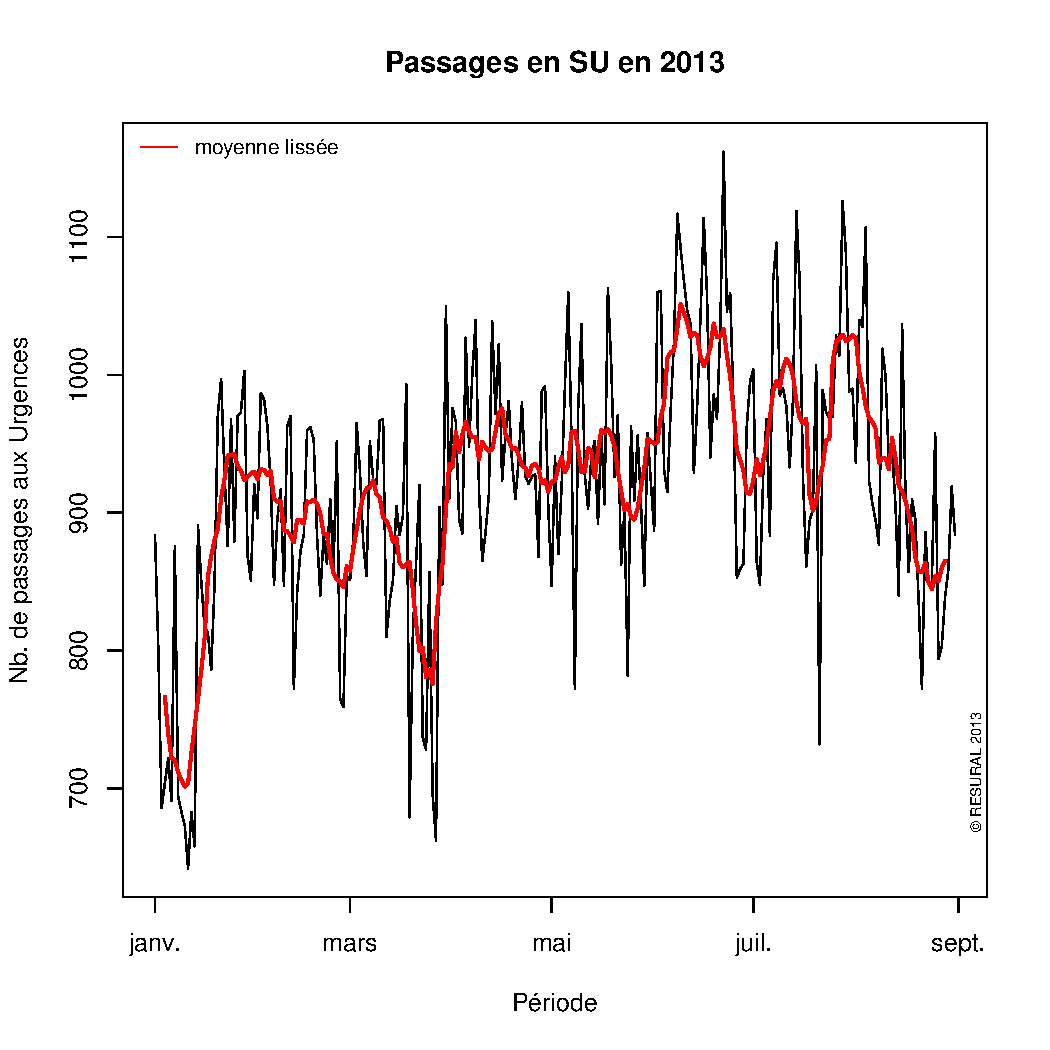
\includegraphics[width=\maxwidth]{figure/activite_plot} 

\end{knitrout}

% Variante avec *xts*
\begin{knitrout}
\definecolor{shadecolor}{rgb}{0.969, 0.969, 0.969}\color{fgcolor}
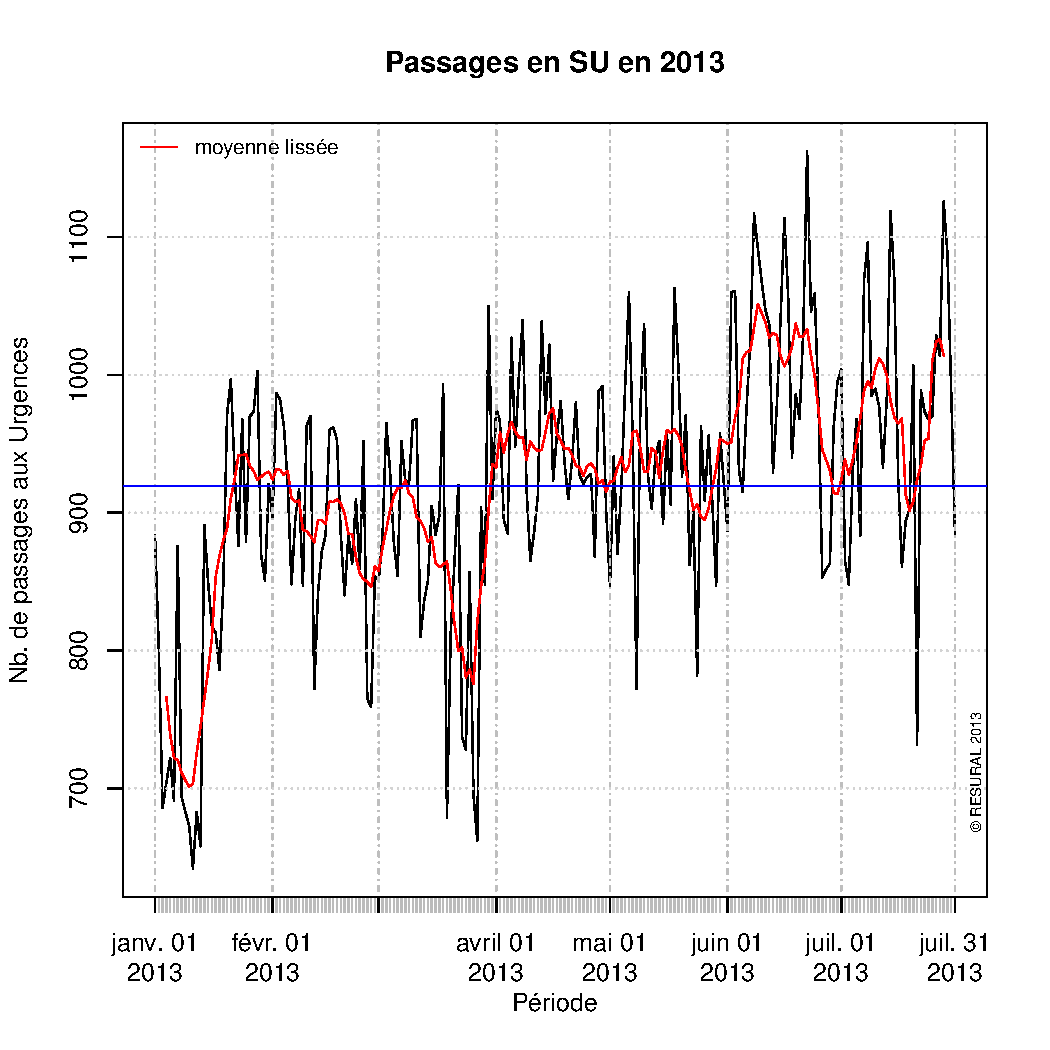
\includegraphics[width=\maxwidth]{figure/activite_plot2} 

\end{knitrout}


\subsection*{En valeur absolue}
\begin{knitrout}
\definecolor{shadecolor}{rgb}{0.969, 0.969, 0.969}\color{fgcolor}\begin{kframe}
\begin{verbatim}
##   3Fr   Alk   Col   Dia   Geb   Hag   Hus   Mul   Odi   Sel   Wis   Sav 
## 10752  4552 44271 19699 10207 23542 25498 36619 17327 18502  8521  2861
\end{verbatim}
\end{kframe}
\end{knitrout}


\subsection*{En pourcentage}
\begin{knitrout}
\definecolor{shadecolor}{rgb}{0.969, 0.969, 0.969}\color{fgcolor}\begin{kframe}
\begin{verbatim}
##   3Fr   Alk   Col   Dia   Geb   Hag   Hus   Mul   Odi   Sel   Wis   Sav 
##  4.84  2.05 19.91  8.86  4.59 10.59 11.47 16.47  7.79  8.32  3.83  1.29
\end{verbatim}
\end{kframe}
\end{knitrout}


\subsection*{Taux de recours aux urgences}
\begin{knitrout}
\definecolor{shadecolor}{rgb}{0.969, 0.969, 0.969}\color{fgcolor}\begin{kframe}
\begin{verbatim}
## [1] 441062
\end{verbatim}
\end{kframe}
\end{knitrout}

Le taux de recours aux urgences \index{taux de recours aux urgences} (TRU) \index{TRU} est défini comme le nombre total de passages aux urgences, rapporté à la population de la région (INSEE 1er janvier 2010). En Lorraine, ce taux est estimé à 23,45\% en 2010 (\cite{2,3}). En supposant que la population alsacienne se comprte comme la population lorraine, le nombre de passages aux urgences devrait s'établir à \ensuremath{4.4106\times 10^{5}}.

Le TRU 2013 estimé en Alsace à partir des RPU transmis est de 11.82\%.

\subsection*{Activité par mois}
%------------------------------
\begin{knitrout}
\definecolor{shadecolor}{rgb}{0.969, 0.969, 0.969}\color{fgcolor}\begin{kframe}
\begin{alltt}
m <- \hlkwd{month}(d1$ENTREE, label = TRUE)
\hlkwd{table}(m)
\end{alltt}
\begin{verbatim}
## m
##   Jan   Feb   Mar   Apr   May   Jun   Jul   Aug   Sep   Oct   Nov   Dec 
## 25609 25004 26937 28428 27899 30038 30103 28333     0     0     0     0
\end{verbatim}
\begin{alltt}
\hlkwd{barplot}(\hlkwd{table}(m), ylab = \hlstr{"nombre"}, xlab = \hlstr{"mois"}, main = \hlstr{"2013 - Nombre de RPU par mois"}, 
    names.arg = \hlkwd{c}(\hlstr{"Jan"}, \hlstr{"Fev"}, \hlstr{"Mar"}, \hlstr{"Avr"}, \hlstr{"Mai"}, \hlstr{"Jui"}, \hlstr{"Jul"}, \hlstr{"Aou"}, \hlstr{"Sep"}, 
        \hlstr{"Oct"}, \hlstr{"Nov"}, \hlstr{"Dec"}), las = 2)
\end{alltt}
\end{kframe}
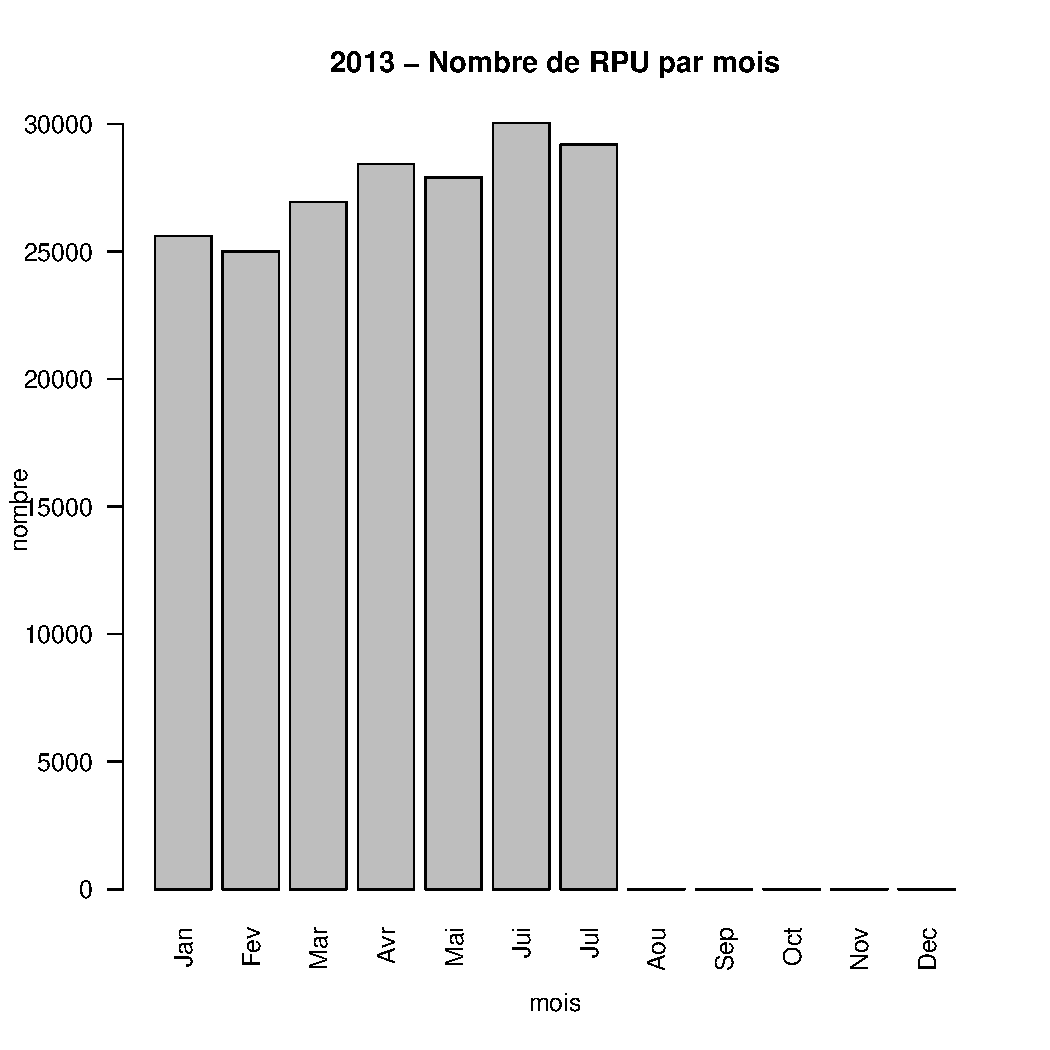
\includegraphics[width=\maxwidth]{figure/parmois} 

\end{knitrout}


\subsection*{Activité par semaine}

% latex table generated in R 2.15.1 by xtable 1.7-1 package
% Wed Sep 18 09:03:40 2013
\begin{table}[ht]
\centering
\begin{tabular}{rr}
  \hline
 & m \\ 
  \hline
1 & 4488 \\ 
  2 & 4909 \\ 
  3 & 5975 \\ 
  4 & 6593 \\ 
  5 & 6509 \\ 
  6 & 6354 \\ 
  7 & 6262 \\ 
  8 & 6193 \\ 
  9 & 6028 \\ 
  10 & 6426 \\ 
  11 & 6152 \\ 
  12 & 5735 \\ 
  13 & 5926 \\ 
  14 & 6698 \\ 
  15 & 6632 \\ 
  16 & 6667 \\ 
  17 & 6538 \\ 
  18 & 6462 \\ 
  19 & 6628 \\ 
  20 & 6720 \\ 
  21 & 6314 \\ 
  22 & 5615 \\ 
  23 & 7116 \\ 
  24 & 7213 \\ 
  25 & 7193 \\ 
  26 & 6569 \\ 
  27 & 6566 \\ 
  28 & 7083 \\ 
  29 & 6391 \\ 
  30 & 7069 \\ 
  31 & 6995 \\ 
  32 & 6726 \\ 
  33 & 6436 \\ 
  34 & 5998 \\ 
  35 & 5172 \\ 
   \hline
\end{tabular}
\caption[Activité par semaine]{Activité des SU par semaine en 2013} 
\label{act_sem}
\end{table}
% latex table generated in R 2.15.1 by xtable 1.7-1 package
% Wed Sep 18 09:03:40 2013
\begin{table}[ht]
\centering
\begin{tabular}{rrrrrrrrrrrrrrrrrrrrrrrrrrrrrrrrrrrr}
  \hline
 & 1 & 2 & 3 & 4 & 5 & 6 & 7 & 8 & 9 & 10 & 11 & 12 & 13 & 14 & 15 & 16 & 17 & 18 & 19 & 20 & 21 & 22 & 23 & 24 & 25 & 26 & 27 & 28 & 29 & 30 & 31 & 32 & 33 & 34 & 35 \\ 
  \hline
1 & 4488 & 4909 & 5975 & 6593 & 6509 & 6354 & 6262 & 6193 & 6028 & 6426 & 6152 & 5735 & 5926 & 6698 & 6632 & 6667 & 6538 & 6462 & 6628 & 6720 & 6314 & 5615 & 7116 & 7213 & 7193 & 6569 & 6566 & 7083 & 6391 & 7069 & 6995 & 6726 & 6436 & 5998 & 5172 \\ 
   \hline
\end{tabular}
\caption[Activité par semaine]{Activité des SU par semaine en 2013} 
\label{act_sem2}
\end{table}

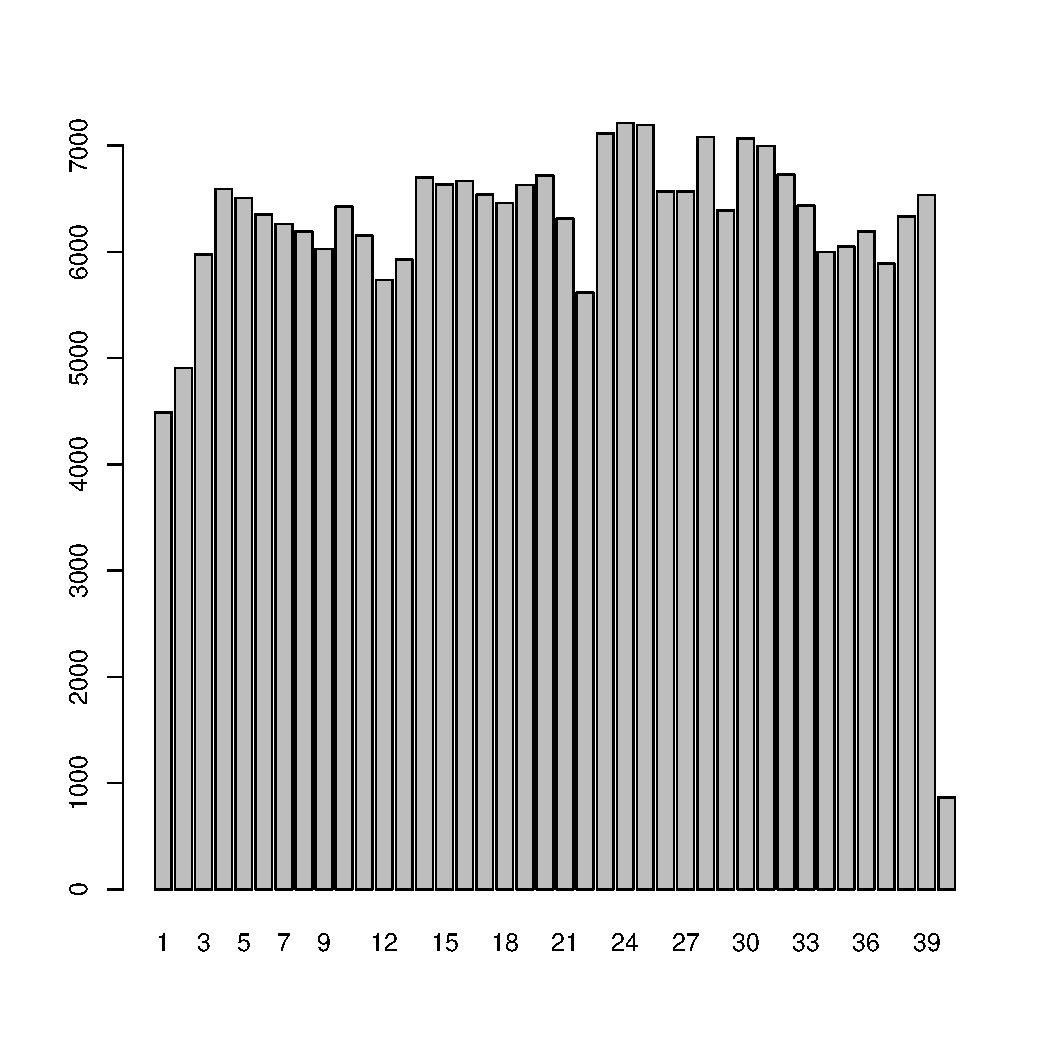
\includegraphics[width=\maxwidth]{figure/act_sem} 



\subsection*{Activité par jour de la semaine}
\begin{knitrout}
\definecolor{shadecolor}{rgb}{0.969, 0.969, 0.969}\color{fgcolor}\begin{kframe}
\begin{alltt}
m <- \hlkwd{wday}(d1$ENTREE, label = T)
\hlkwd{table}(m)
\end{alltt}
\begin{verbatim}
## m
##   Sun   Mon  Tues   Wed Thurs   Fri   Sat 
## 32332 33648 31238 30166 31385 30745 32837
\end{verbatim}
\begin{alltt}
\hlkwd{barplot}(\hlkwd{table}(m), names.arg = \hlkwd{c}(\hlstr{"Dim"}, \hlstr{"Lun"}, \hlstr{"Mar"}, \hlstr{"Mer"}, \hlstr{"Jeu"}, \hlstr{"Ven"}, \hlstr{"Sam"}))
\end{alltt}
\end{kframe}
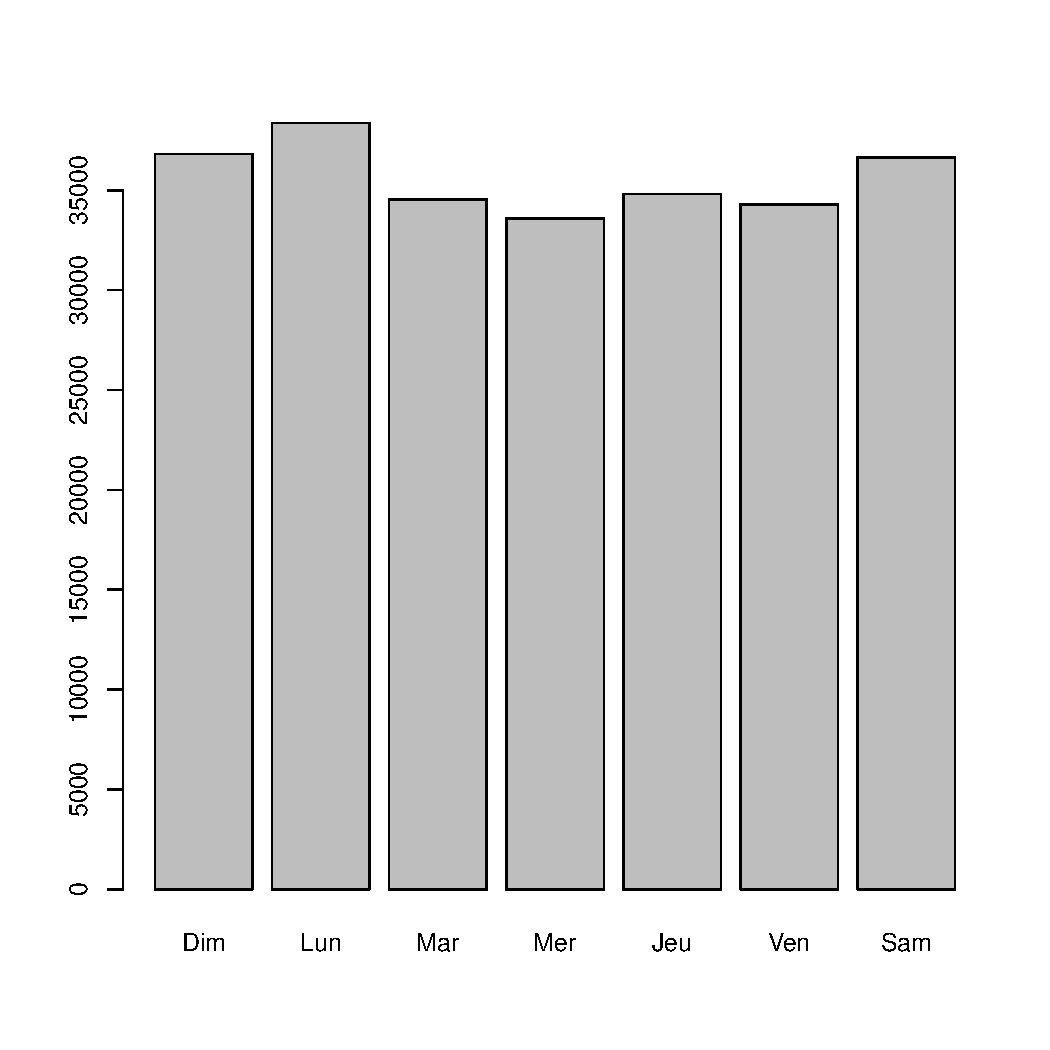
\includegraphics[width=\maxwidth]{figure/activite_semaine} 

\end{knitrout}


\subsection*{Activité horaire}
\begin{knitrout}
\definecolor{shadecolor}{rgb}{0.969, 0.969, 0.969}\color{fgcolor}
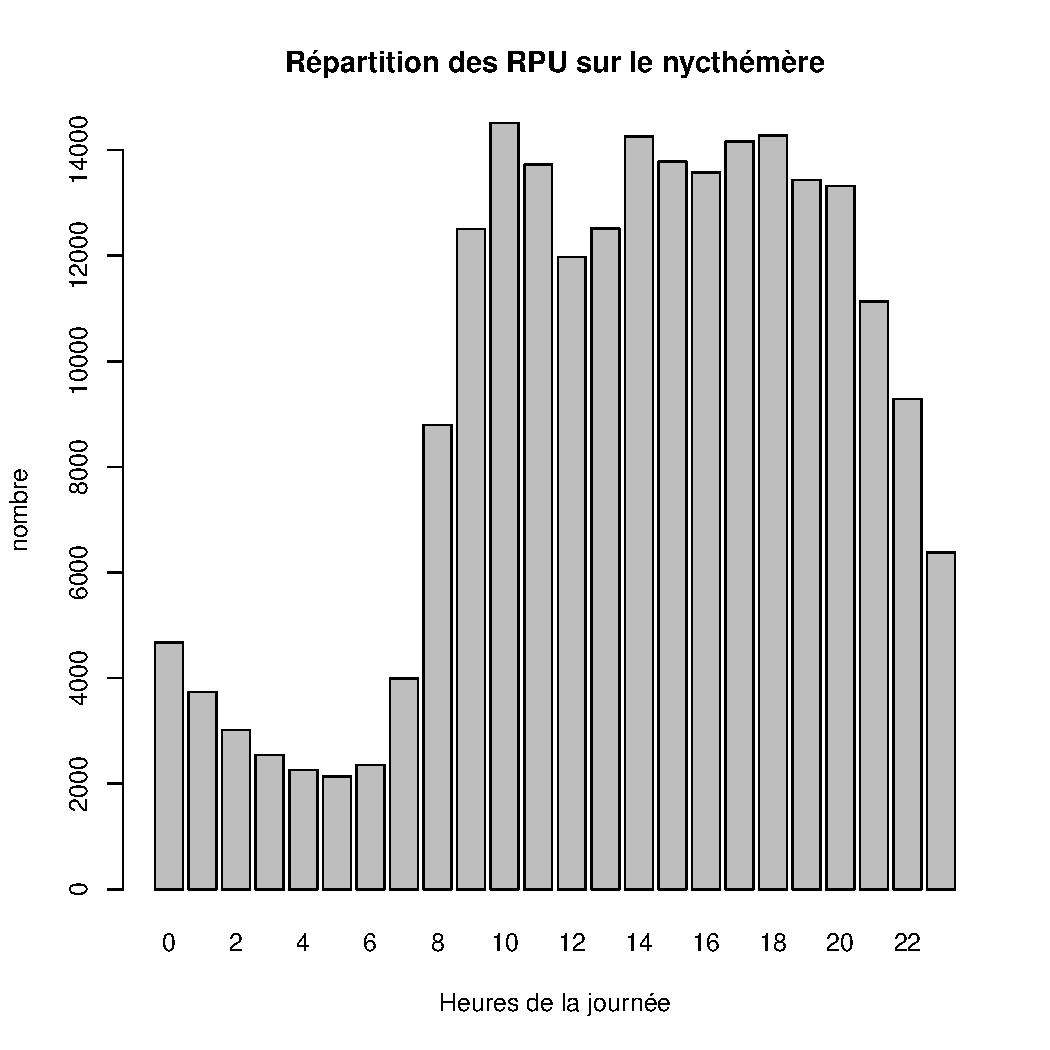
\includegraphics[width=\maxwidth]{figure/activite_heure} 

\end{knitrout}


  

\section{TEST 2}

% test2.Rnw

L'activité horaire des services d'urgence en Alsace est totalement superposable à celui de l'ensemble des SU (figure \ref{passage:als} page \pageref{passage:als}). L'activité diminue fortement en nuit profonde à partir de une heure du matin pour redémarrer vers 9 heures et s'intensifier progressivement en matinée. Après un premier pic en fin de matinée, la croissance reprend pour culminer vers 19 heures, puis décroître lentement jusqu'en fin de soirée.

Ce phénomène cyclique se répète tous les jours selon un profil immuable. La projection de ces données sur un graphique en radar représentant les 24 tranches horaires (figure \ref{radar:als} page \pageref{radar:als}) montre qu'il existe trois pics d'égale amplitude à 11, 15 et 19 heures. Ce point mérite d'être analysé car s'il se confirme, cela pourrait indiquer que le pointage de 11 heures permet d'avoir une prévision sur l'intensité de la fréquentation avant la garde du soir. On peut en rapprocher le fait que la médiane des passages se situe vers 14h, c'est à dire qu'au ointage de 15 heures on peut évaluer la quantité totale de patients qui vont se présenter dans les heures qui viennent.

%----------------------------------------------------------------------------- Summary
Résumé des horaires de passage aux ugences: les données figurent dans le tableau \ref{tab:24} page \pageref{tab:24}.
% latex table generated in R 2.15.1 by xtable 1.7-1 package
% Wed Sep 18 09:03:46 2013
\begin{table}[ht]
\centering
\begin{tabular}{rrrrrrrrr}
  \hline
 & n & Min & Q25 & Moyenne & E-type & Médiane & Q75 & Max \\ 
  \hline
 & 222351.00 & 0.00 & 10.00 & 13.90 & 5.60 & 14.00 & 18.00 & 23.00 \\ 
   \hline
\end{tabular}
\caption[horaires de passage]{Résumé des horaires de passage aux urgences} 
\label{tab:24}
\end{table}



\input{../blah.gen}
%---------------------------------------------------------------------- HISTOGRAMME

\begin{figure}
\begin{center}
\begin{knitrout}
\definecolor{shadecolor}{rgb}{0.969, 0.969, 0.969}\color{fgcolor}
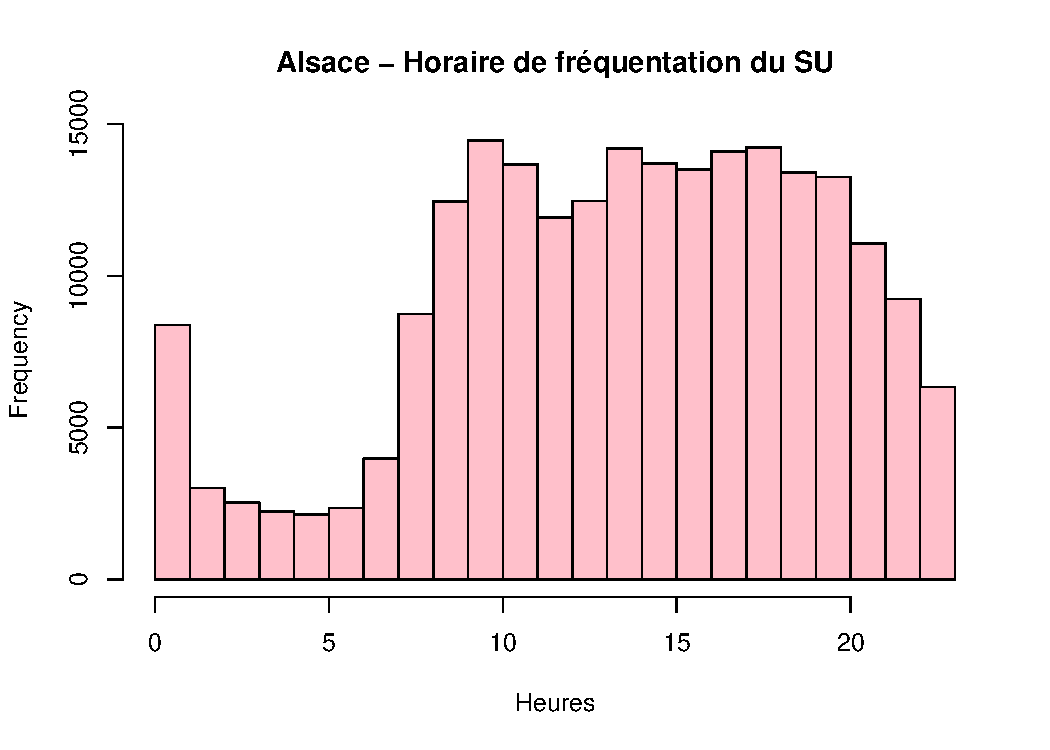
\includegraphics[width=\maxwidth]{figure/test23} 

\end{knitrout}

\end{center}
\caption{Horaires d'arrivée aux urgences en Alsace 2013}
\label{passage:als}
\end{figure}
%---------------------------------------------------------------------------- RADAR 1

\begin{figure}
\begin{center}
\begin{knitrout}
\definecolor{shadecolor}{rgb}{0.969, 0.969, 0.969}\color{fgcolor}
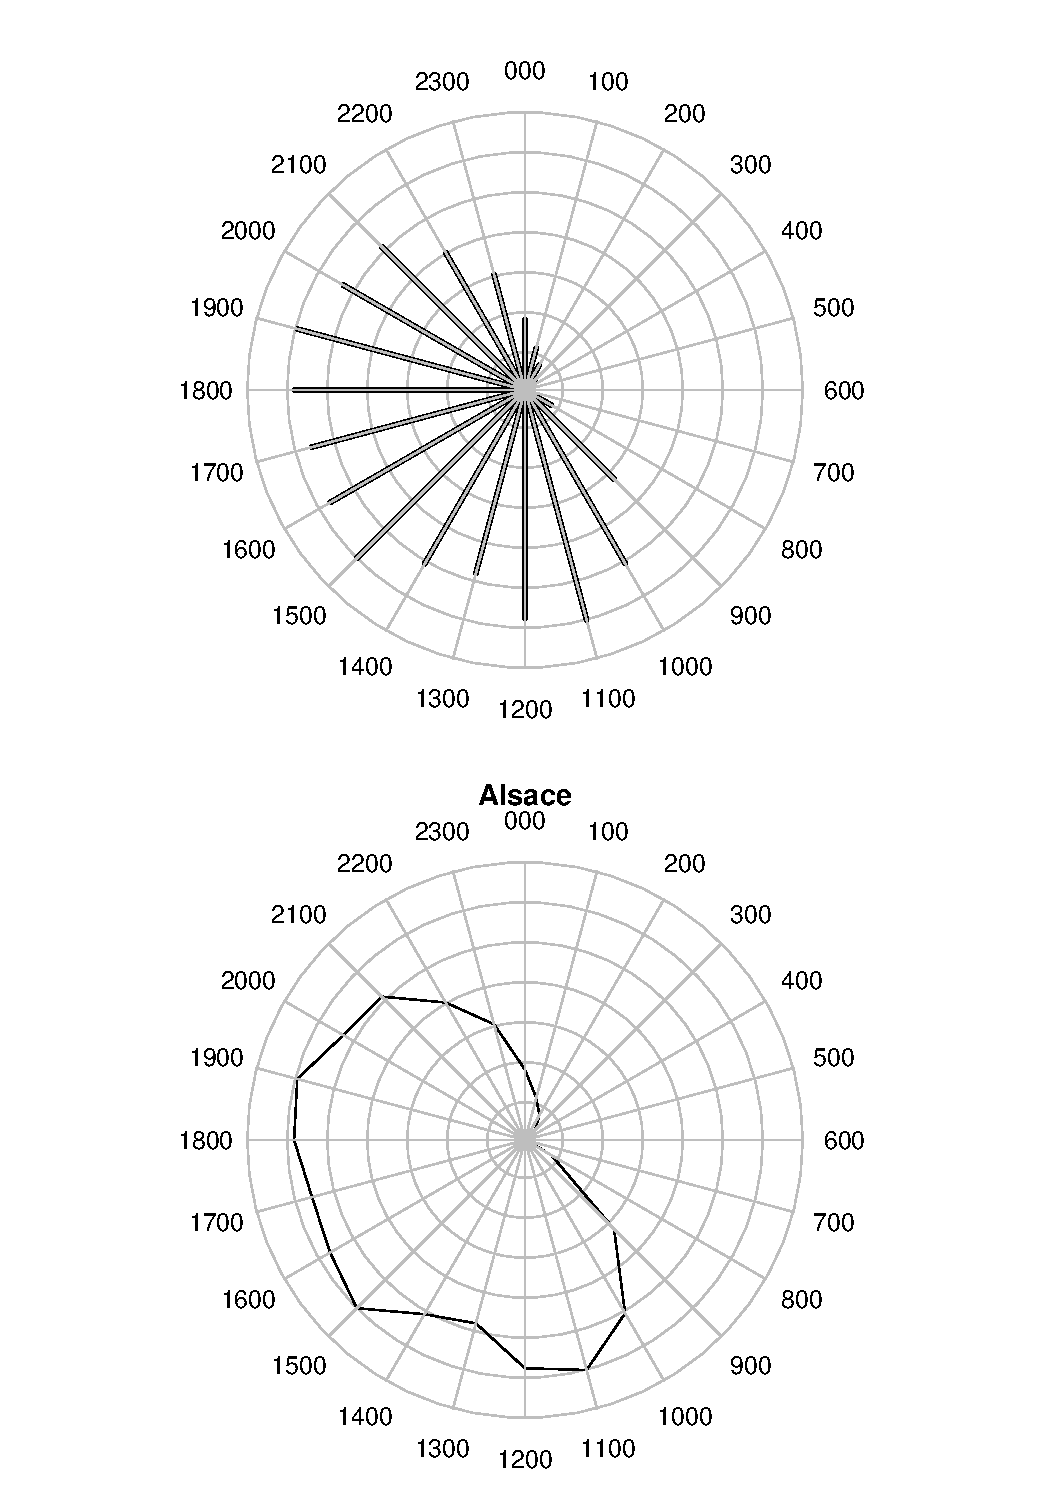
\includegraphics[width=\maxwidth]{figure/test25} 

\end{knitrout}

\end{center}
\caption{Horaires d'arrivée aux urgences en Alsace 2013}
\label{radar:als}
\end{figure}

%---------------------------------------------------------Radar HUS
\begin{figure}
\begin{center}
\begin{knitrout}
\definecolor{shadecolor}{rgb}{0.969, 0.969, 0.969}\color{fgcolor}
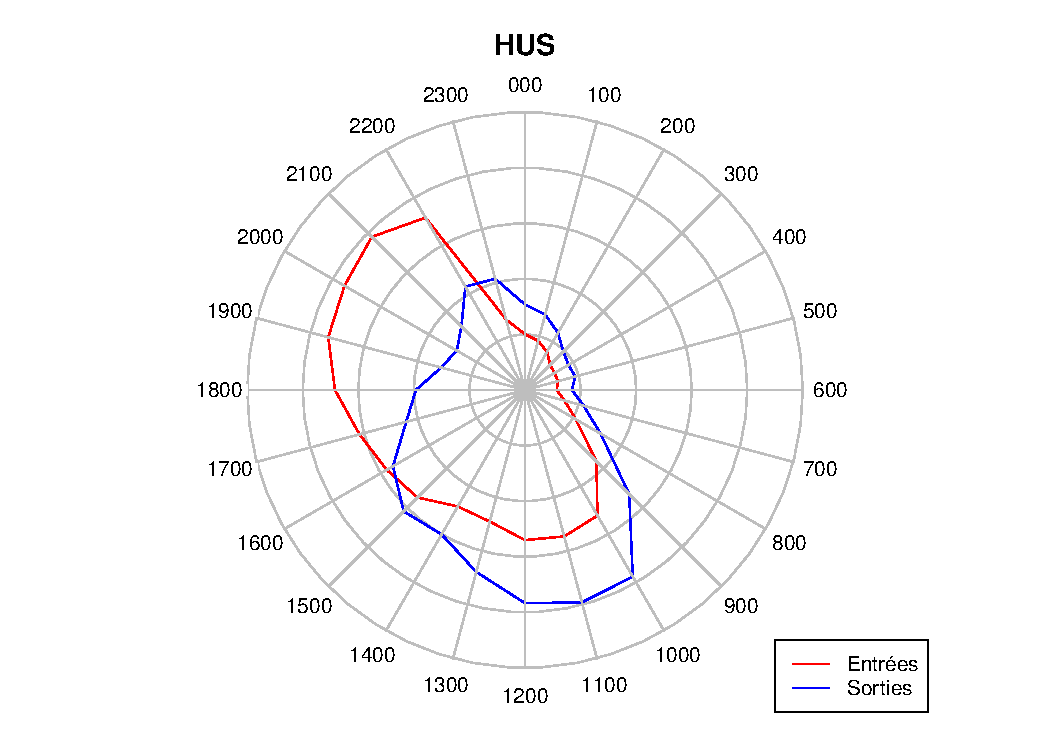
\includegraphics[width=\maxwidth]{figure/test2} 

\end{knitrout}

\end{center}
\caption{HUS: répartition des arrivées et départs aux urgences}
\label{passage:hus}
\end{figure}

%----------------------------------------------------------------
\begin{figure}
\begin{center}
\begin{knitrout}
\definecolor{shadecolor}{rgb}{0.969, 0.969, 0.969}\color{fgcolor}
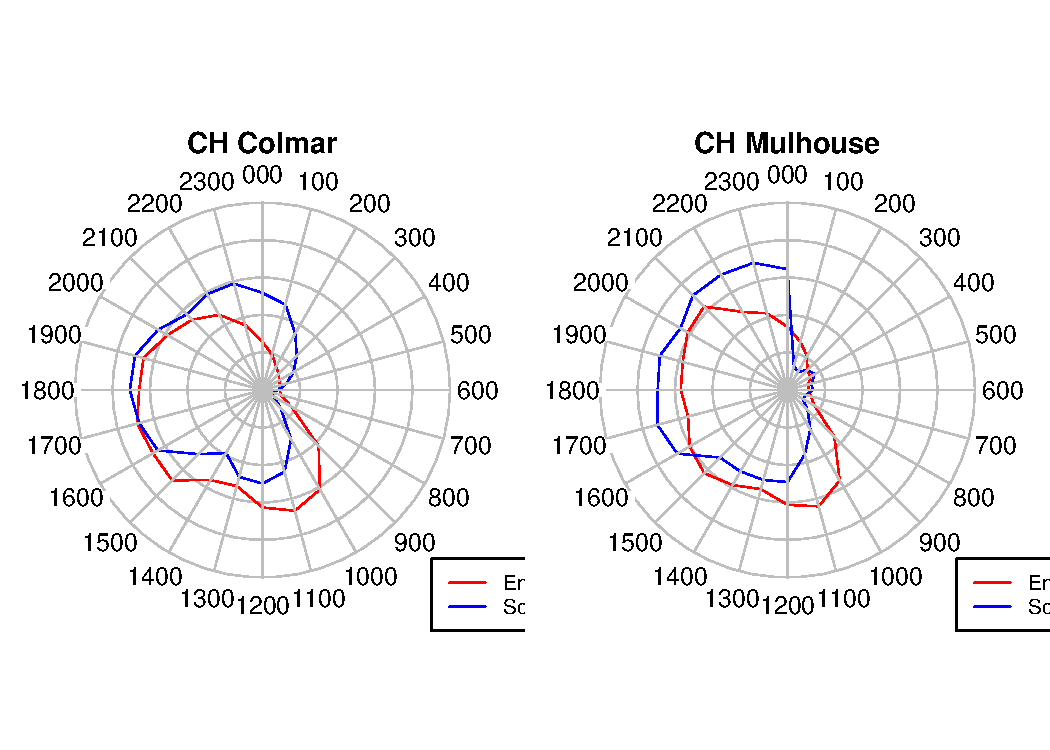
\includegraphics[width=\maxwidth]{figure/test22} 

\end{knitrout}

\end{center}
\caption{CH Colmar et Mulhouse: répartition des arrivées et départs aux urgences}
\label{passage:col}
\end{figure}




\subsection{Passages par tranches d'âge}

\chapter{Modalité d'admission}

% modalites.Rnw
% modalités d'admission MODE_ENTREE

\index{Mode d'entrée}

\section*{Origine des patients}
% REMARQUE dans environ 300 dossiers du mois de juin, l'item transfert est écrit "transfe  rt" ce qui nécessite un recodage.

L'immense majorité des patients provient du domicile ou son équivalent. Une très faible part des passages aux urgences sont le fait de transferts d'autres établissements ou de mutations en provenance d'autres services du même établissement.


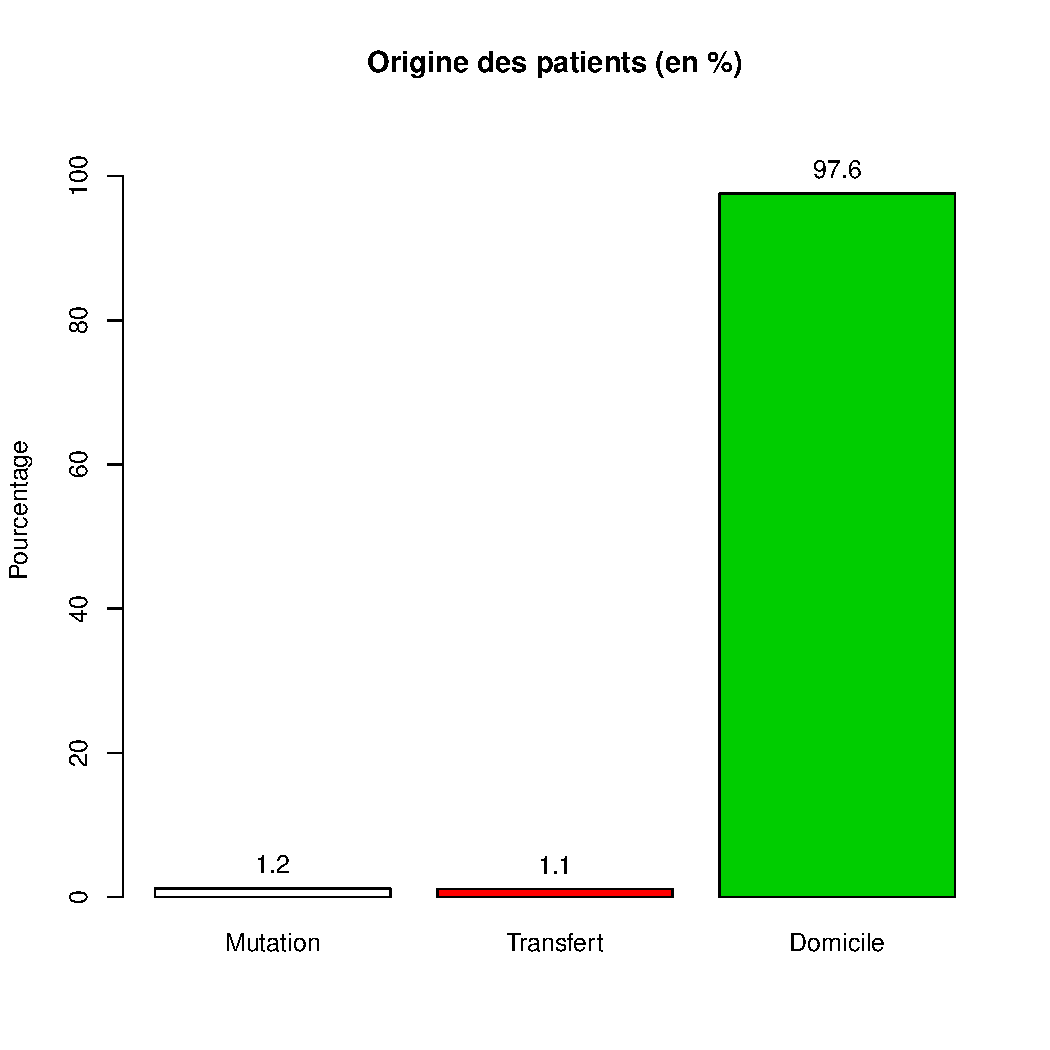
\includegraphics[width=\maxwidth]{figure/mode_entree} 
% latex table generated in R 2.15.1 by xtable 1.7-1 package
% Wed Sep 18 09:03:50 2013
\begin{table}[ht]
\centering
\begin{tabular}{rrrr}
  \hline
 & Frequency &   \%(NA+) &   \%(NA-) \\ 
  \hline
Mutation & 2433.00 & 1.10 & 1.20 \\ 
  Transfert & 2255.00 & 1.00 & 1.10 \\ 
  Domicile & 193838.00 & 87.20 & 97.60 \\ 
  NA's & 23825.00 & 10.70 & 0.00 \\ 
    Total & 222351.00 & 100.00 & 100.00 \\ 
   \hline
\end{tabular}
\caption[Origine des patients]{Origine des patients. Les deux colonnes de droite mesurent l'origine (en pourcentage) selon que l'on prenne en compte ou non les valeurs manquantes. } 
\label{origine}
\end{table}



Dans 10.7 \% des cas, l'origine du patient n'est pas précisée.

\section*{Mode de transport}
\index{Mode de transport}

La grande majorité des patients arrivent aux urgences par leurs propres moyens (PERSO). Lorsqu'ils font appel à un tiers, il s'agit le plus souvent d'une ambulance privée (AMBU), puis du SDIS (AMBU). Les transports par un vecteur médicalisé (SMUR) ou héliporté (HELI) sont rares. Enfin l'utilisation des forces de l'ordre (FO) comme moyen de transport reste marginale.


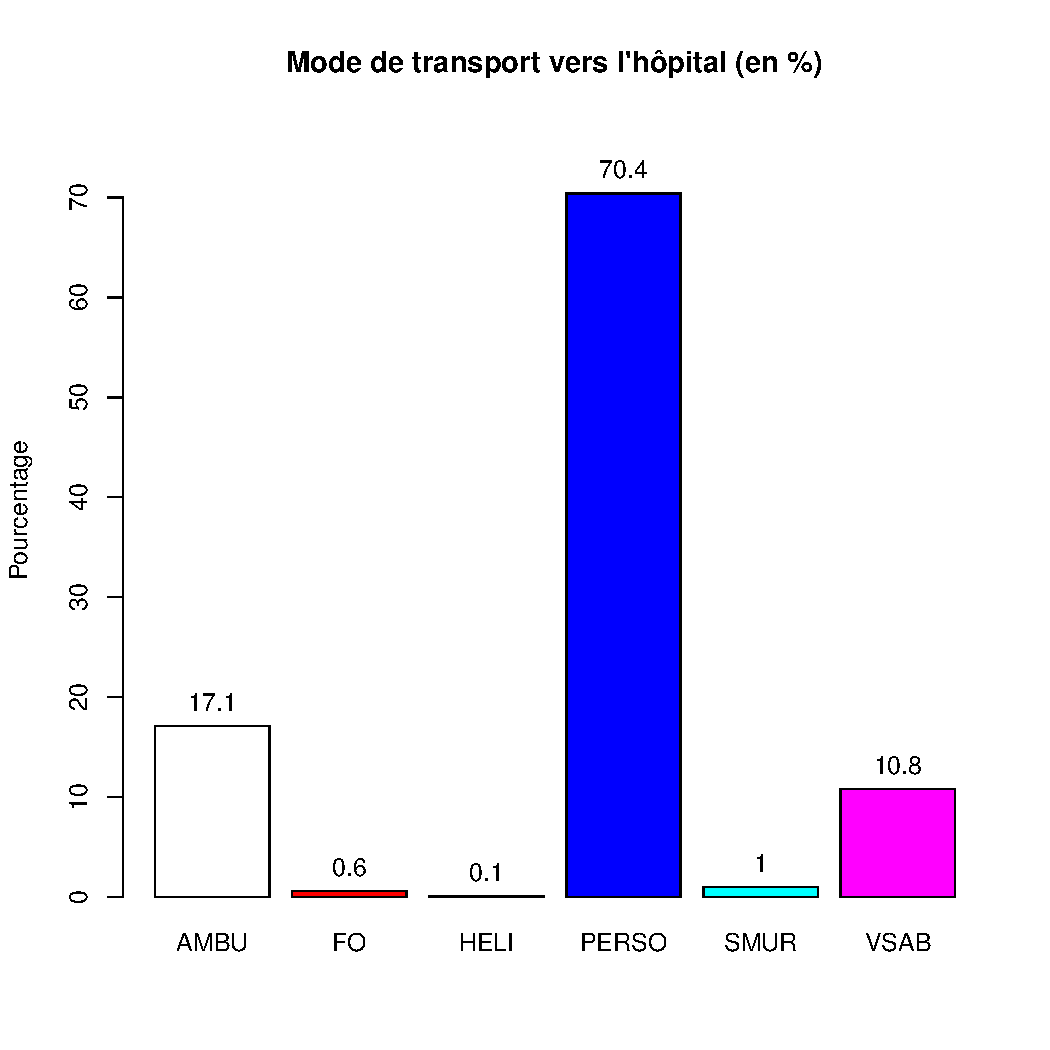
\includegraphics[width=\maxwidth]{figure/transport} 
% latex table generated in R 2.15.1 by xtable 1.7-1 package
% Wed Sep 18 09:03:50 2013
\begin{table}[ht]
\centering
\begin{tabular}{rrrr}
  \hline
 & Frequency &   \%(NA+) &   \%(NA-) \\ 
  \hline
AMBU & 30257.00 & 13.60 & 17.30 \\ 
  FO & 975.00 & 0.40 & 0.60 \\ 
  HELI & 147.00 & 0.10 & 0.10 \\ 
  PERSO & 123229.00 & 55.40 & 70.30 \\ 
  SMUR & 1860.00 & 0.80 & 1.10 \\ 
  VSAB & 18834.00 & 8.50 & 10.70 \\ 
  NA's & 47049.00 & 21.20 & 0.00 \\ 
    Total & 222351.00 & 100.00 & 100.00 \\ 
   \hline
\end{tabular}
\caption[Moyens de transport]{Moyens de transport utilisés pour se rendre à l'hôpital. Les deux colonnes de droite mesurent la fréquence du moyen utilise (en pourcentage) selon que l'on prenne en compte ou non les valeurs manquantes. } 
\label{transport}
\end{table}



Dans 21.2 \% des cas, le moyen de transport utilisé par le patient pour rejoindre l'hôpial n'est pas précisé.

\section*{Origine géographique}



Les patients consultant aux urgences sont majoritairement issus de la région Alsace. Mais l'origine est très diverse, aussi bien en provenance des autres départements français qu'hors de France:
% \begin{itemize}
%   \item Alsace: cp_als (\Sexpr(round(cp_als*100/n,2) \%))
%   \item hors Alsace: cp_hals
%   \item dont hors de France: cp_monde
% \end{itemize}



\chapter{Durée de passage}

% duree_passage.Rnw

La durée de passage est le temps compris entre la date d'entrée et celle de sortie. Il s'agit d'une durée de transit total. Les données transmises par les RPU ne permettent pas de calculer les temps d'attenre.

\begin{knitrout}
\definecolor{shadecolor}{rgb}{0.969, 0.969, 0.969}\color{fgcolor}\begin{kframe}


{\ttfamily\noindent\color{warningcolor}{\#\# Warning: All formats failed to parse. No formats found.}}\begin{verbatim}
##    Min. 1st Qu.  Median    Mean 3rd Qu.    Max.    NA's 
##       1      86     137     162     216     974     627
\end{verbatim}
\end{kframe}
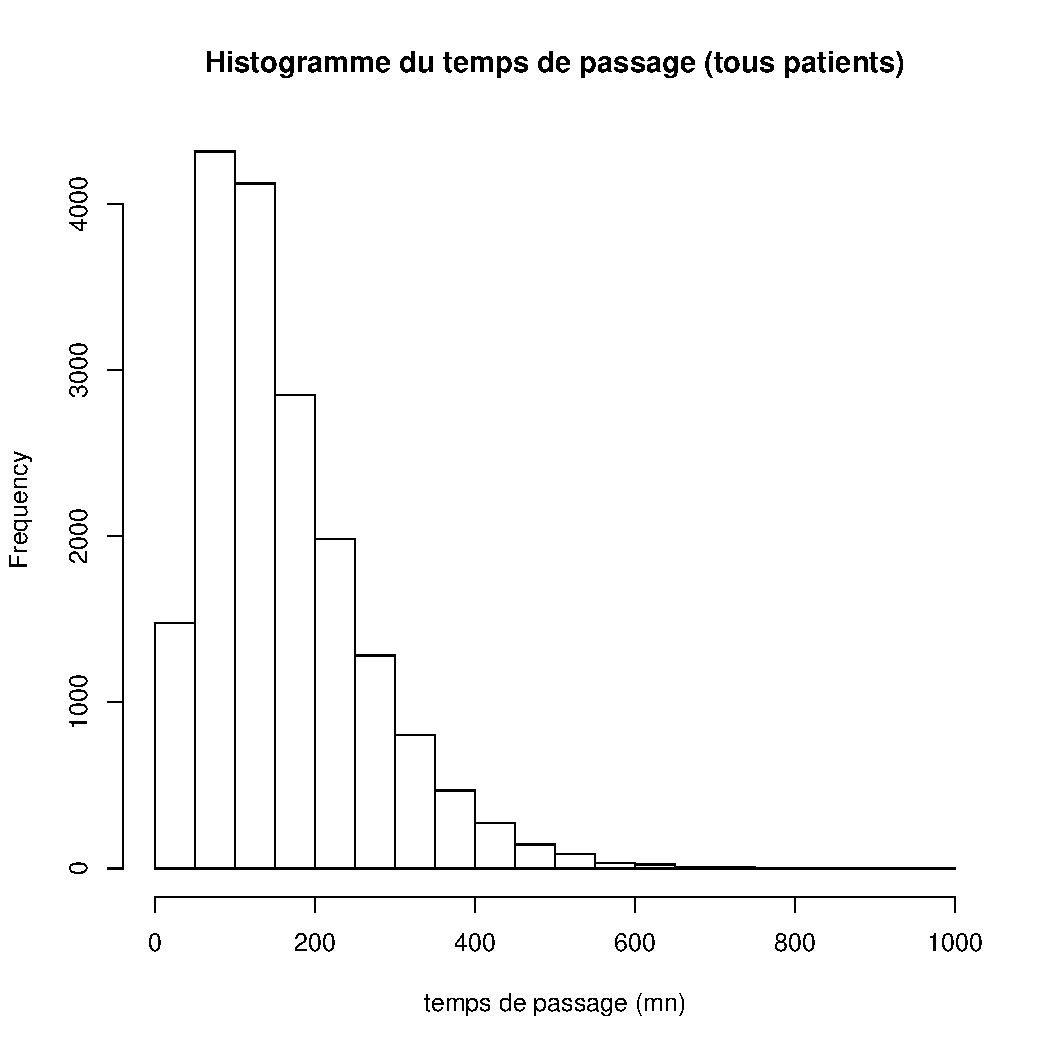
\includegraphics[width=\maxwidth]{figure/passage} 

\end{knitrout}



% RPU_2013_analyse à partir de la ligne 382

\section*{Selon l'heure}

Une période de 24 heures est habituellement divisée de la manière suivante:
\begin{enumerate}
  \item \emph{journée} de 8 heures à 20 heures
  \item \emph{soirée} de 20 heures à minuit
  \item  \emph{nuit profonde} de 0 heures à 8 heures
\end{enumerate}

\begin{knitrout}
\definecolor{shadecolor}{rgb}{0.969, 0.969, 0.969}\color{fgcolor}\begin{kframe}
\begin{verbatim}
## nuit profonde       journée        soirée          NA's 
##          2455         13592          2082           373
\end{verbatim}
\end{kframe}
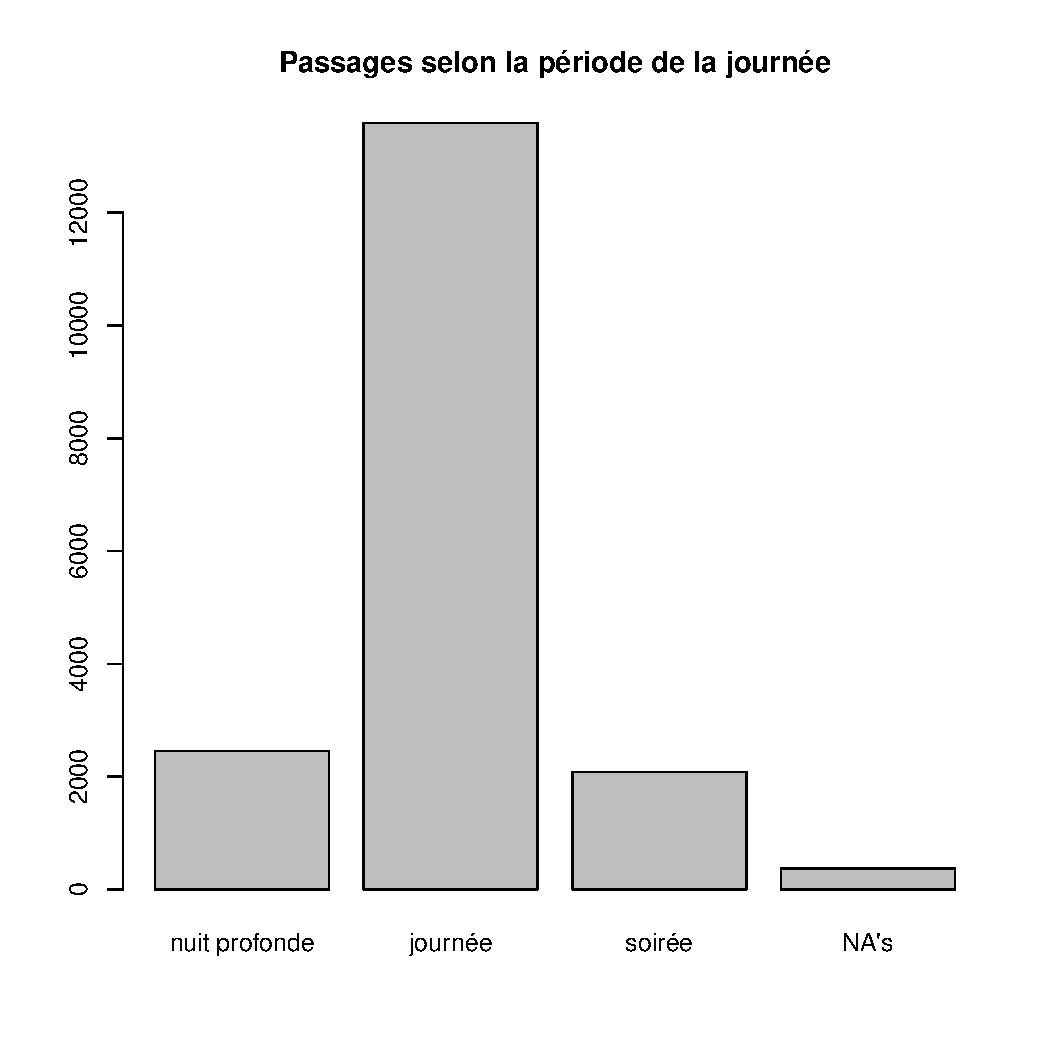
\includegraphics[width=\maxwidth]{figure/duree_heure1} 
\begin{kframe}\begin{verbatim}
## nuit profonde       journée        soirée 
##         153.8         168.3         137.2
\end{verbatim}
\end{kframe}
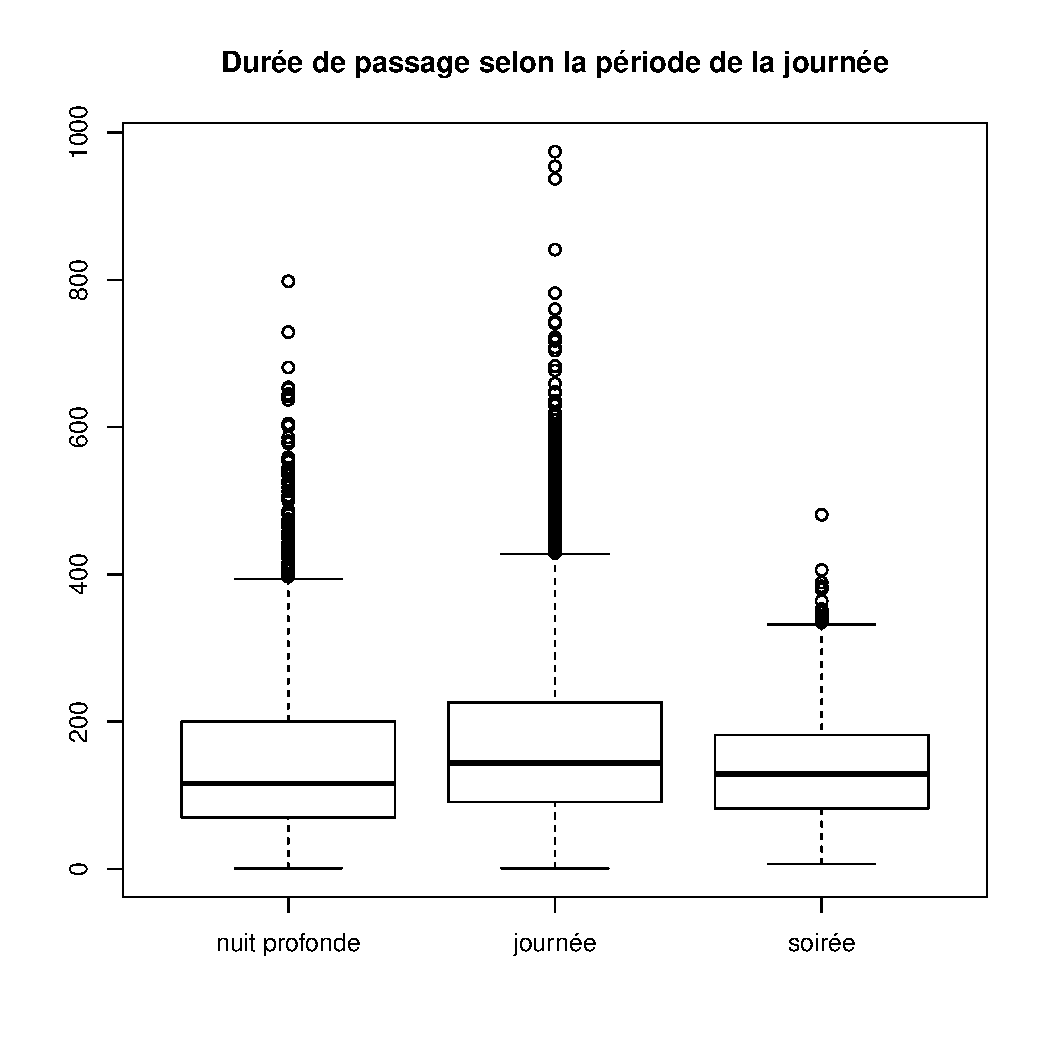
\includegraphics[width=\maxwidth]{figure/duree_heure2} 

\end{knitrout}



\section*{Selon l'âge}

Le temps de passage augmente avec l'age.
\begin{knitrout}
\definecolor{shadecolor}{rgb}{0.969, 0.969, 0.969}\color{fgcolor}\begin{kframe}
\begin{verbatim}
## 15 ans et moins     16 à 74 ans  75 ans et plus            NA's 
##            4406           11399            2392             305
## 15 ans et moins     16 à 74 ans  75 ans et plus 
##           119.6           163.0           244.8
\end{verbatim}
\end{kframe}
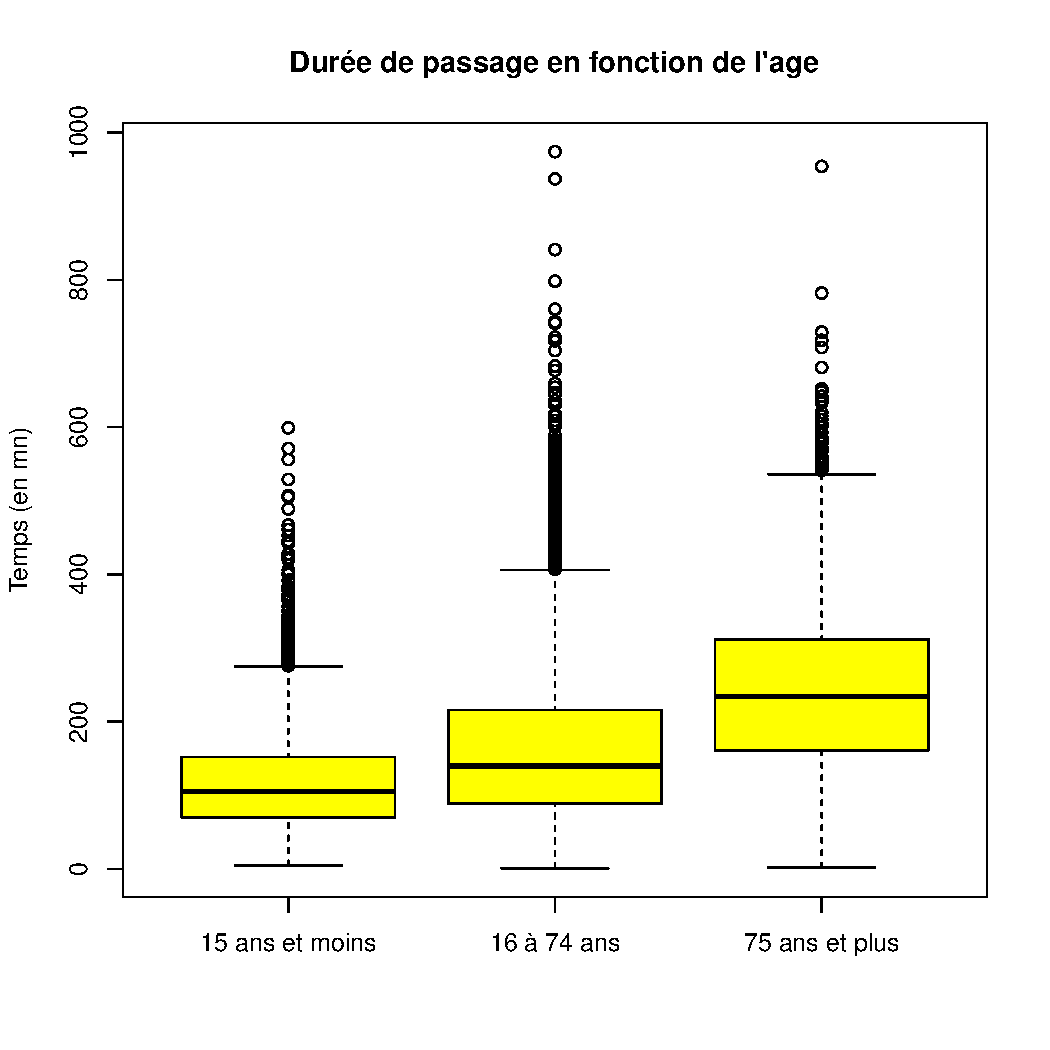
\includegraphics[width=\maxwidth]{figure/duree_age} 

\end{knitrout}


\section*{Selon le jour de la semaine}
\begin{knitrout}
\definecolor{shadecolor}{rgb}{0.969, 0.969, 0.969}\color{fgcolor}\begin{kframe}
\begin{verbatim}
##   Sun   Mon  Tues   Wed Thurs   Fri   Sat 
## 142.9 174.8 167.4 159.9 165.3 158.5 165.3
##                
## periode          Sun  Mon Tues  Wed Thurs  Fri  Sat
##   nuit profonde  430  383  368  290   298  331  355
##   journée       2130 2142 1933 1777  1793 1742 2075
##   soirée         282  272  319  279   282  339  309
\end{verbatim}
\end{kframe}
\end{knitrout}


\subsection*{Pourcentage de passages en moins de 4 heures par établissement}



80.33\% des patients quittent les urgences en moins de quatre heures.

\section*{Selon l'orientation}
\begin{knitrout}
\definecolor{shadecolor}{rgb}{0.969, 0.969, 0.969}\color{fgcolor}\begin{kframe}
\begin{verbatim}
##  CHIR FUGUE   HDT    HO   MED  OBST   PSA   REA   REO    SC  SCAM    SI 
## 186.9 114.5    NA    NA 226.4 164.1 177.3 196.9    NA 280.0 158.3 193.2 
##  UHCD 
## 197.8
##   DOM   MCO   SLD 
## 147.3 215.1 208.5
\end{verbatim}
\end{kframe}
\end{knitrout}



\section*{Selon la gravité}
\begin{knitrout}
\definecolor{shadecolor}{rgb}{0.969, 0.969, 0.969}\color{fgcolor}\begin{kframe}
\begin{verbatim}
##     1     2     3     4     5     D     P 
## 106.1 152.1 220.4 213.8 220.0  42.5 151.1
\end{verbatim}
\end{kframe}
\end{knitrout}


\section*{Selon la structure}
\subsection{CH Sélestat}
\begin{knitrout}
\definecolor{shadecolor}{rgb}{0.969, 0.969, 0.969}\color{fgcolor}\begin{kframe}
\begin{verbatim}
##    Min. 1st Qu.  Median    Mean 3rd Qu.    Max.    NA's 
##       1      86     137     162     216     974     627
\end{verbatim}
\end{kframe}
\end{knitrout}



\chapter{Codage diagnostique}

%




Les motifs de recours aux urgences sont exprimés en fonction de la classification CIM10 \cite{10}.
\index{motis de recours}
\footnote{Classification Internationale des Maladies, 10ème révision (La CIM10 comporte environ 36000 maladies).}.
\url{http://apps.who.int/classifications/icd10/browse/2008/fr}
Le fichier comporte \np{151577} diagnostics principaux différents.
répartis en 4178 classes de diagnostics.
La comparaison entre le nombre de RPU reçus et le nombre de diagnostics renseignés permet d'établir l'exhaustivité des CIM10 à 68.17\% \index{exhaustivité!CIM10}


\section{Cim10}

Ventilation des diagnostics principaux en fonction des 22 chapitres de la CIM10. Le tableau qui suit indique pour chaque chapitre, le nombre total de cas rapportés, le pourcentage par rapport à l'ensemble, et le pourcentage de cas déduction faite de la traumatologie. En effet celleci représente environ la moitié des cas et il parait intéressant de séparer les pathologies traumatiques des non traumatiques.





%round(prop.table(tr)*100,digits=2)

\begin{longtable}{|c|c|m{4cm}|c|c|c|}
 \hline
 Chapitre & Bloc & Titre & N & \% total  & \% non trauma \\
 \hline
 
I & A00–B99 & Certaines maladies infectieuses et parasitaires & 7198 & 4.75 & 10.53 \\
 II&C00–D48&Tumeurs&688&0.45&1.01\\
 
III&D50–D89&Maladies du sang et des organes hématopoïétiques et certains troubles du système immunitaire&306&0.2&0.45\\

IV&E00–E90&Maladies endocriniennes, nutritionnelles et métaboliques&1698&1.12&2.48\\

V&F00–F99&Troubles mentaux et du comportement&7788&5.14&11.39\\

VI&G00–G99&Maladies du système nerveux&4373&2.89&6.4\\

VII & H00–H59 & Maladies de l'oeil et de ses annexes & 4606 & 3.04&6.74\\

VIII&H60–H95&Maladies de l'oreille et de l'apophyse mastoïde&3352&2.21&4.9\\

IX&I00–I99&Maladies de l'appareil circulatoire&9068&5.98&13.26\\

X&J00–J99&Maladies de l'appareil respiratoire&16207&10.69&23.7\\

XI&K00–K93&Maladies de l'appareil digestif&11891&7.84&17.39\\

XII&L00–L99&Maladies de la peau et du tissu cellulaire souscutané&4452&2.94&6.51\\

XIII&M00–M99&Maladies du système ostéoarticulaire, des muscles et du tissu conjonctif&13511&8.91&19.76\\

XIV&N00–N99&Maladies de l'appareil génitourinaire&7610&5.02&11.13\\

XV&O00–O99&Grossesse, accouchement et puerpéralité&252&0.17&0.37\\

XVI&P00–P96&Certaines affections dont l'origine se situe dans la période périnatale&277&0.18&0.41\\

% XVII&Q00–Q99&Malformations congénitales et anomalies chromosomiques&cong&round(cong*100/total,digits=2)&round(cong*100/(total-traumato),digits=2)\\

XVIII&R00–R99&Symptômes, signes et résultats anormaux d'examens cliniques et de laboratoire, non classés ailleurs&34334&22.65&50.22\\

XIX&S00–T98&Lésions traumatiques, empoisonnements et certaines autres conséquences de causes externes&83205&54.89& \\

XX&V01–Y98&Causes externes de morbidité et de mortalité& 3896&2.57&5.7\\

XXI&Z00–Z99&Facteurs influant sur l'état de santé et motifs de recours aux services de santé&6502&4.29&4.29\\

XXII&U00–U99&Codes d'utilisation particulière & 0&0&0\\

  \hline
\end{longtable}



\begin{knitrout}
\definecolor{shadecolor}{rgb}{0.969, 0.969, 0.969}\color{fgcolor}
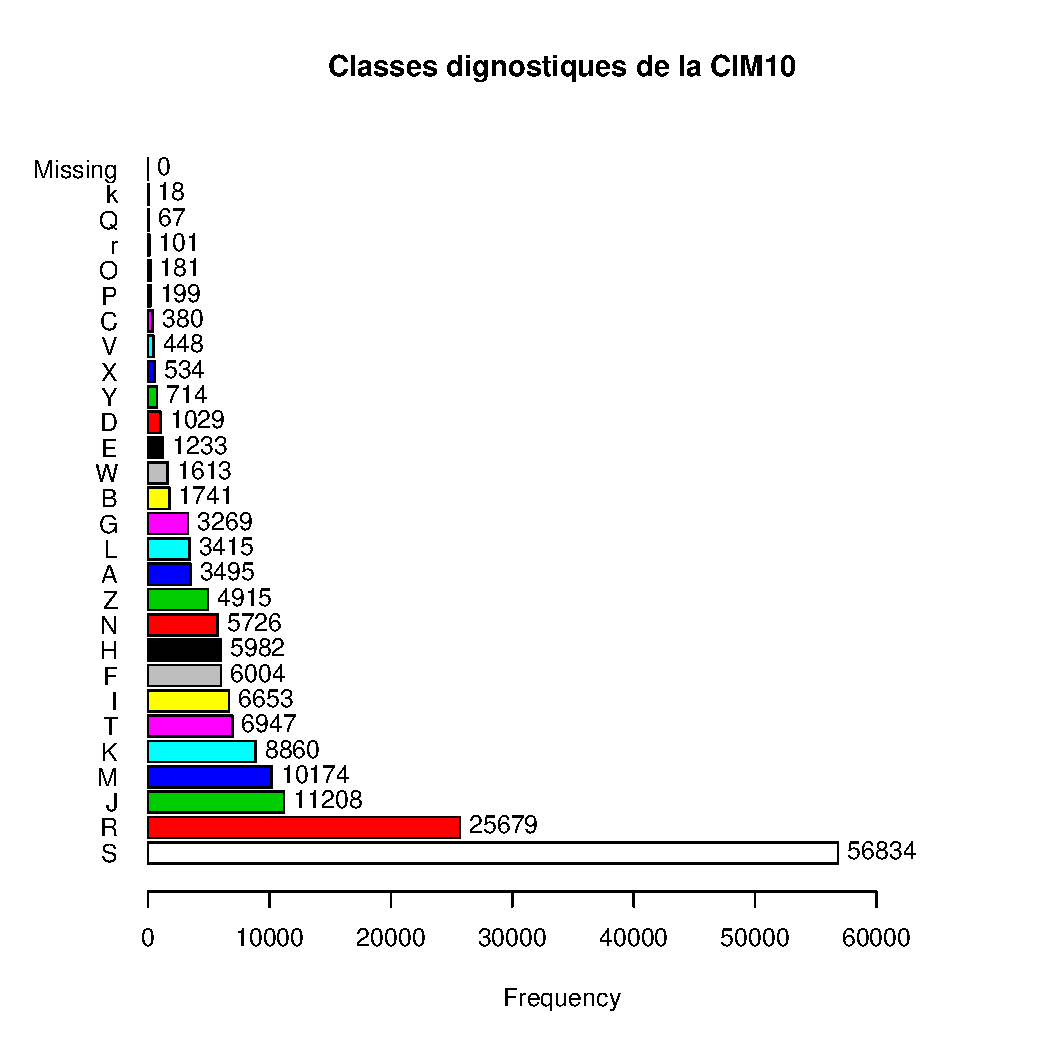
\includegraphics[width=\maxwidth]{figure/class_cim10} 
\begin{kframe}\begin{verbatim}
## a :  
##         Frequency Percent Cum. percent
## S           51428    33.9         33.9
## R           23202    15.3         49.2
## J           10215     6.7         56.0
## M            9224     6.1         62.1
## K            8052     5.3         67.4
## T            6261     4.1         71.5
## I            6004     4.0         75.5
## H            5493     3.6         79.1
## F            5400     3.6         82.7
## N            5215     3.4         86.1
## Z            4405     2.9         89.0
## A            3202     2.1         91.1
## L            3100     2.0         93.2
## G            2956     2.0         95.1
## B            1613     1.1         96.2
## W            1439     0.9         97.1
## E            1123     0.7         97.9
## D             915     0.6         98.5
## Y             609     0.4         98.9
## X             463     0.3         99.2
## V             385     0.3         99.4
## C             344     0.2         99.7
## P             187     0.1         99.8
## O             171     0.1         99.9
## r              94     0.1         99.9
## Q              61     0.0        100.0
## k              16     0.0        100.0
##   Total    151577   100.0        100.0
\end{verbatim}
\end{kframe}
\end{knitrout}


\section{Etude des AVC}

\index{AVC}
Les AVC sont définis par la nomenclature I60 à I64, G45 Accidents ischémiques cérébraux transitoires (sauf G45.4 amnésie transitoire) et syndromes apparentés et G46 Syndromes vasculaires cérébraux au cours de maladies cérébrovasculaires

La prévention et la prise en charge des accidents vasculaires cérébraux  Annexes 
juin 2009

Annexe : Liste exhaustive des codes CIM10 d’AVC

\begin{longtable}{|l|l|}
 \hline
 Code & libellé\\
 \hline
 G450 & Syndrome vertébrobasilaire \\
 G451 & Syndrome carotidien (hémisphérique) \\
 G452 & Accident ischémique transitoire de territoires artériels précérébraux multiples et bilatéraux \\
 G453 & Amaurose fugace \\
 G454 & Amnésie globale transitoire : NON RETENU \\
 G458 & Autres accidents ischémiques cérébraux transitoires et syndromes apparentés \\
 G459 & Accident ischémique cérébral transitoire, sans précision \\
 I600 & Hémorragie sousarachnoïdienne de labifurcation et du siphon carotidien \\
 I601 & Hémorragie sousarachnoïdienne de l'artère cérébrale moyenne \\
 I602 & Hémorragie sousarachnoïdienne de l'artère communicante antérieure \\
 I603 & Hémorragie sousarachnoïdienne del'artère communicante postérieure \\
 I604 & Hémorragie sousarachnoïdienne de l'artère basilaire \\
 I605 & Hémorragie sousarachnoïdienne de l'artère vertébrale \\
 I606 & Hémorragie sousarachnoïdienne d'autres artères intracrâniennes \\
 I607 & Hémorragie sousarachnoïdienne d'une artère intracrânienne, sans précision \\
 I608 & Autres hémorragies sousarachnoïdiennes \\
 I609 & Hémorragie sousarachnoïdienne, sans précision \\
 I610 & Hémorragie intracérébrale hémisphérique, souscorticale \\
 I611 & Hémorragie intracérébrale hémisphérique, corticale \\
 I612 & Hémorragie intracérébrale hémisphérique, non précisée \\
 I613 & Hémorragie intracérébrale du tronc cérébral \\
 I614 & Hémorragie intracérébrale cérébelleuse \\
 I615 & Hémorragie intracérébrale intraventriculaire \\
 I616 & Hémorragie intracérébrale,localisations multiples \\
 I618 & Autres hémorragies intracérébrales \\
 I619 & Hémorragie intracérébrale, sans précision \\
 I620 & Hémorragie sousdurale (aiguë) (non traumatique) \\
 I621 & Hémorragie extradurale non traumatique \\
 I629 & Hémorragie intracrânienne (non traumatique), sans précision \\
 I630 & Infarctus cérébral dû à une thrombose des artères précérébrales \\
 I631 & Infarctus cérébral dû à une embolie des artères précérébrales \\
 I632 & Infarctus cérébral dû à une occlusion ou sténose des artères précérébrales,de mécanisme non précisé \\
 I633 & Infarctus cérébral dû à une thrombose des artères cérébrales \\
 I634 & Infarctus cérébral dû à une embolie des artères cérébrales \\
 I635 & Infarctus cérébral dû à une occlusion ou sténose des artères cérébrales, demécanisme non précisé \\
 I636 & Infarctus cérébral dû à une thrombose veineuse cérébrale, non pyogène \\
 I638 & Autres infarctus cérébraux \\
 I639 & Infarctus cérébral, sans précision \\
 I64 & Accident vasculaire cérébral, non précisé comme étant hémorragique ou par infarctus \\
 G460 & Syndrome de l'artère cérébrale moyenne (I66.0) (1) \\
 G461 & Syndrome de l'artère cérébrale antérieure (I66.1) (1) \\
 G462 & Syndrome de l'artère cérébrale postérieure (I66.2) (1) \\
 G463 & Syndromes vasculaires du tronc cérébral (I60I67) (1) \\
 G464 & Syndrome cérébelleux vasculaire (I60I67) (1) \\
 G465 & Syndrome lacunaire moteur pur (I60I67) (1) \\
 G466 & Syndrome lacunaire sensitif pur (I60I67) (1) \\
 G467 & Autres syndromes lacunaires (I60I67) (1) \\
 G468 & Autres syndromes vasculaires cérébraux au cours de maladies cérébrovasculaires (I60I67) (1) \\
  \hline
\end{longtable}

\begin{knitrout}
\definecolor{shadecolor}{rgb}{0.969, 0.969, 0.969}\color{fgcolor}\begin{kframe}
\begin{alltt}
\hlcom{# Création d'un dataframe DP}
dpr <- d1[!\hlkwd{is.na}(d1$DP), \hlkwd{c}(\hlstr{"DP"}, \hlstr{"CODE_POSTAL"}, \hlstr{"ENTREE"}, \hlstr{"FINESS"}, \hlstr{"GRAVITE"}, 
    \hlstr{"ORIENTATION"}, \hlstr{"MODE_SORTIE"}, \hlstr{"AGE"}, \hlstr{"SEXE"}, \hlstr{"TRANSPORT"})]
\hlcom{# correction d'erreurs:}
dpr$DP[37807] <- \hlstr{"N10"}
dpr$DP[47689] <- \hlstr{"R06.0"}
dpr$DP[68023] <- \hlstr{"C61"}
dpr$DP[73924] <- \hlstr{"N10"}
\hlcom{# un peu de ménage:}
dpr$DP <- \hlkwd{gsub}(\hlstr{"."}, \hlstr{""}, \hlkwd{as.character}(dpr$DP), fixed = TRUE)
dpr$DP <- \hlkwd{gsub}(\hlstr{"+"}, \hlstr{""}, \hlkwd{as.character}(dpr$DP), fixed = TRUE)
\hlcom{# extraction d'un DF avc:}
AVC <- dpr[\hlkwd{substr}(dpr$DP, 1, 3) >= \hlstr{"I60"} & \hlkwd{substr}(dpr$DP, 1, 3) < \hlstr{"I65"} | \hlkwd{substr}(dpr$DP, 
    1, 3) == \hlstr{"G46"} | \hlkwd{substr}(dpr$DP, 1, 3) == \hlstr{"G45"}, ]
\end{alltt}
\end{kframe}
\end{knitrout}


\subsection*{Horaire des AVC}
\index{AVC!heure}

Horaire des AVC, à comparer avec:
\begin{itemize}
  \item les crises d'épilepsie
  \item la pression athmosphérique
\end{itemize}

\begin{knitrout}
\definecolor{shadecolor}{rgb}{0.969, 0.969, 0.969}\color{fgcolor}
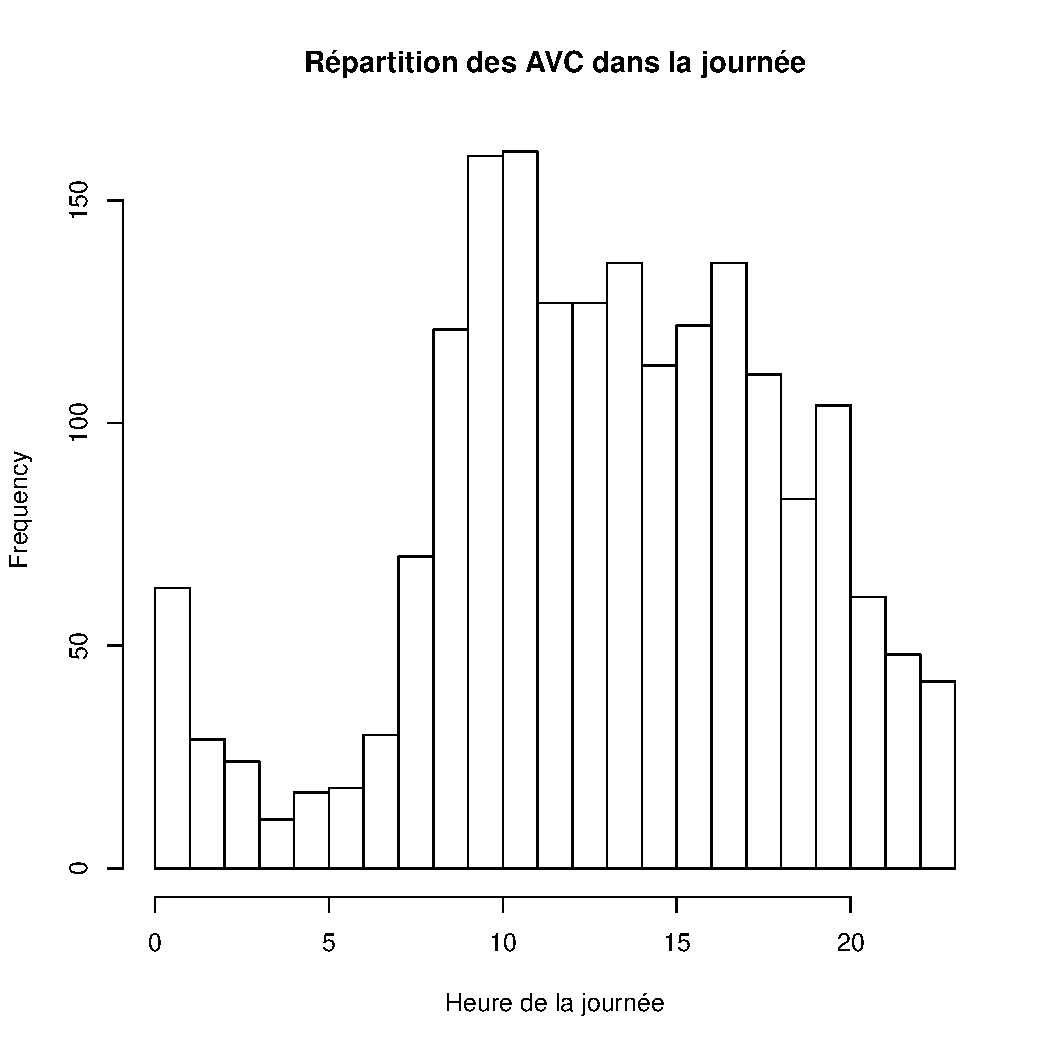
\includegraphics[width=\maxwidth]{figure/heure_avc1} 

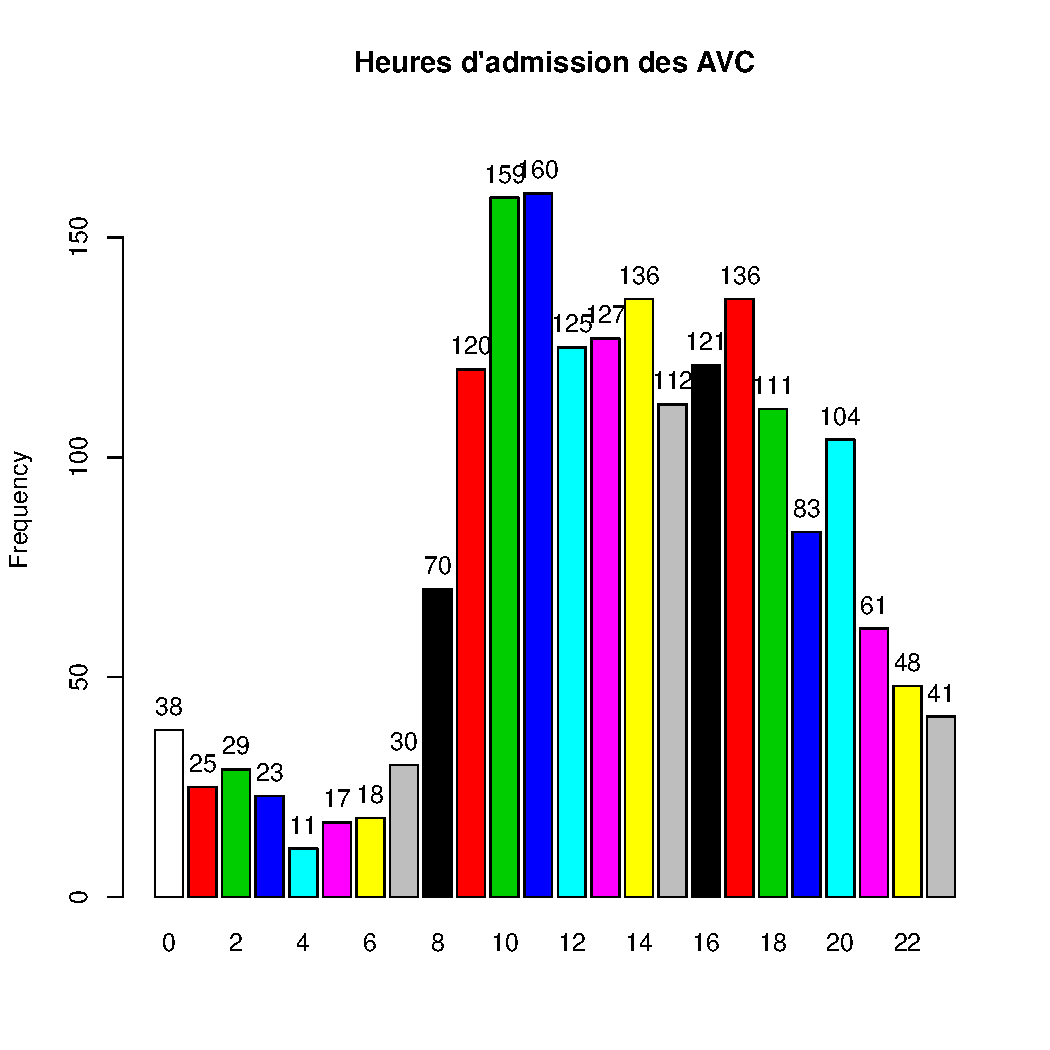
\includegraphics[width=\maxwidth]{figure/heure_avc2} 
\begin{kframe}\begin{verbatim}
## h :  
##         Frequency Percent Cum. percent
## 0              38     2.0          2.0
## 1              25     1.3          3.3
## 2              29     1.5          4.8
## 3              24     1.3          6.1
## 4              11     0.6          6.6
## 5              17     0.9          7.5
## 6              18     0.9          8.5
## 7              30     1.6         10.0
## 8              70     3.7         13.7
## 9             121     6.3         20.0
## 10            160     8.4         28.4
## 11            161     8.4         36.8
## 12            127     6.6         43.4
## 13            127     6.6         50.1
## 14            136     7.1         57.2
## 15            113     5.9         63.1
## 16            122     6.4         69.4
## 17            136     7.1         76.5
## 18            111     5.8         82.3
## 19             83     4.3         86.7
## 20            104     5.4         92.1
## 21             61     3.2         95.3
## 22             48     2.5         97.8
## 23             42     2.2        100.0
##   Total      1914   100.0        100.0
\end{verbatim}
\end{kframe}
\end{knitrout}


\subsection*{Selon le jour de la semaine}
\index{AVC!age}

\begin{knitrout}
\definecolor{shadecolor}{rgb}{0.969, 0.969, 0.969}\color{fgcolor}\begin{kframe}
\begin{verbatim}
## w
## Dim Lun Mar Mer Jeu Ven Sam 
## 228 295 298 290 288 268 247
## w
##   Dim   Lun   Mar   Mer   Jeu   Ven   Sam 
## 11.91 15.41 15.57 15.15 15.05 14.00 12.90
\end{verbatim}
\end{kframe}
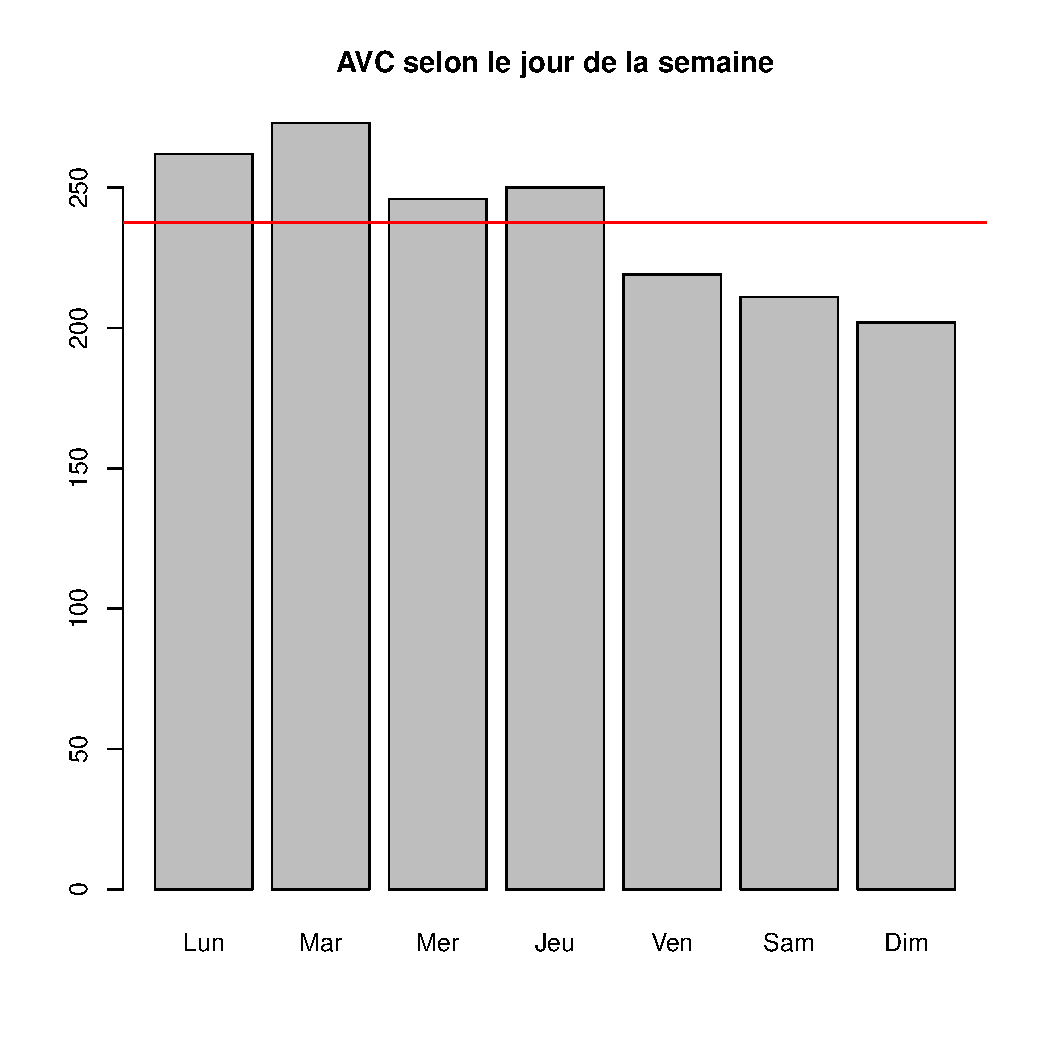
\includegraphics[width=\maxwidth]{figure/avc_jour_semaine} 

\end{knitrout}

Proportion théorique = 14.28\% par jour de la semaine.

\subsection*{AVC et age}
\index{AVC!age}
\begin{knitrout}
\definecolor{shadecolor}{rgb}{0.969, 0.969, 0.969}\color{fgcolor}\begin{kframe}
\begin{verbatim}
##    Min. 1st Qu.  Median    Mean 3rd Qu.    Max. 
##     1.0    61.0    75.0    70.8    83.0   112.0
\end{verbatim}
\end{kframe}
\end{knitrout}

Le rapport de 2009 donne age moyen = 70.5 et age médian = 75 ans.

\subsection*{AVC et sexe}
\index{AVC!sexe}
\begin{knitrout}
\definecolor{shadecolor}{rgb}{0.969, 0.969, 0.969}\color{fgcolor}\begin{kframe}
\begin{verbatim}
##   F   I   M 
## 993   0 921
\end{verbatim}
\end{kframe}
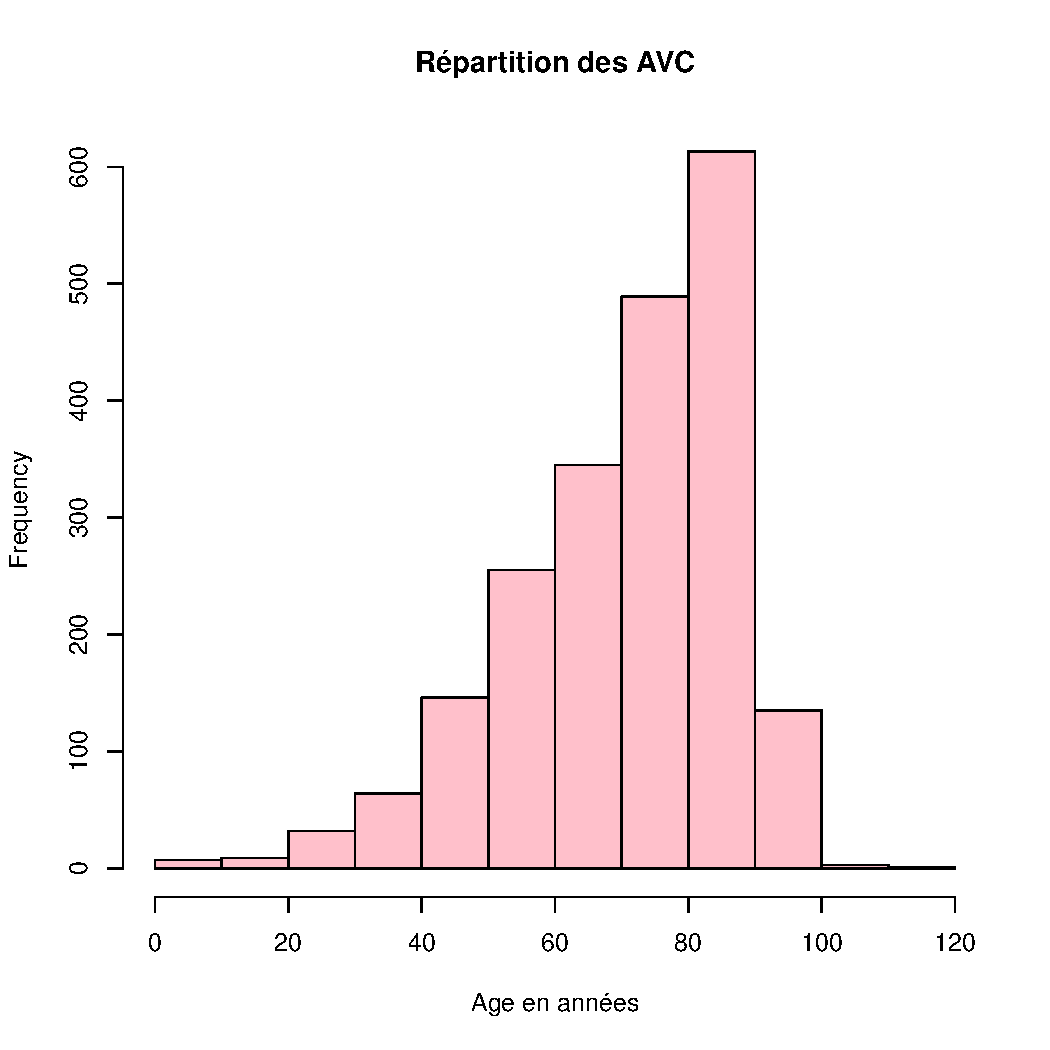
\includegraphics[width=\maxwidth]{figure/avc_sexe1} 

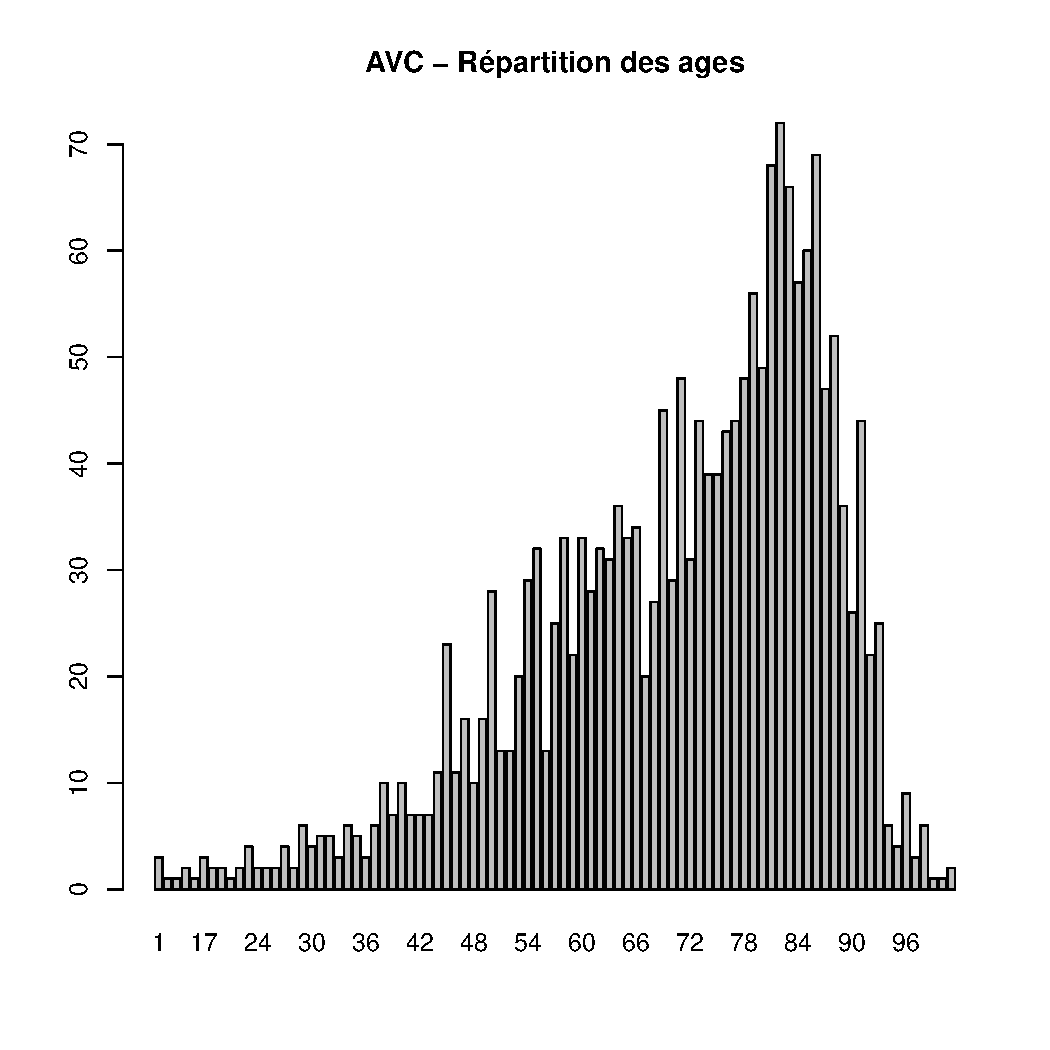
\includegraphics[width=\maxwidth]{figure/avc_sexe2} 

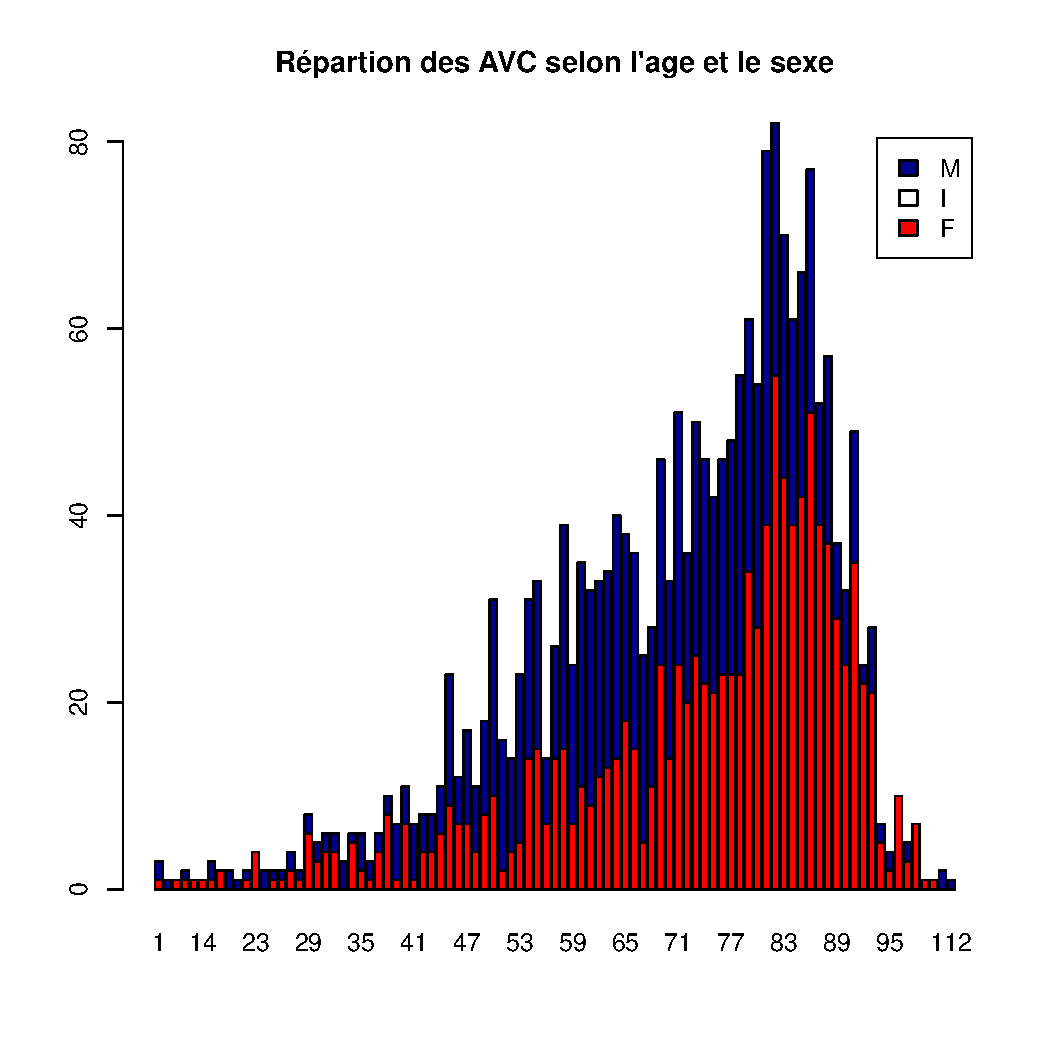
\includegraphics[width=\maxwidth]{figure/avc_sexe3} 

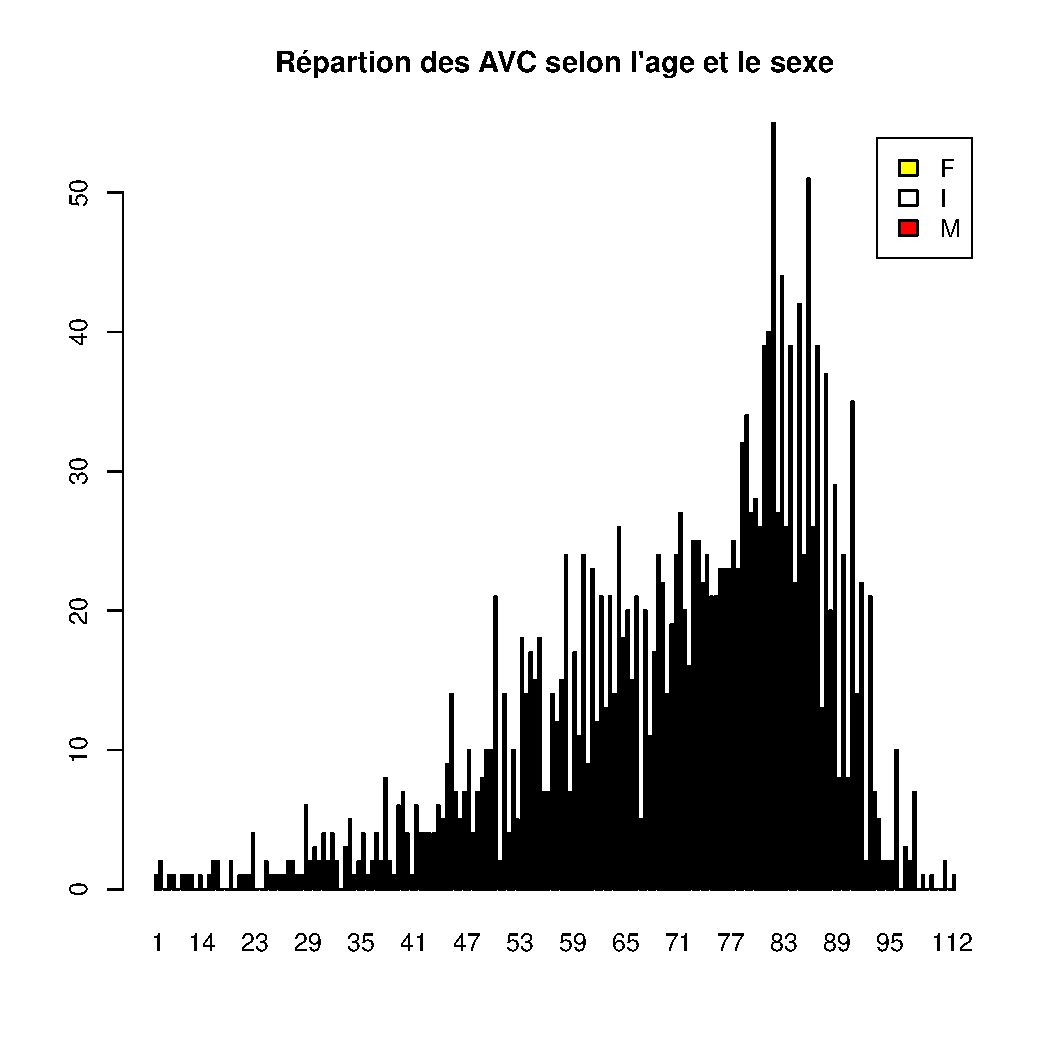
\includegraphics[width=\maxwidth]{figure/avc_sexe4} 

\end{knitrout}


\section{Accidents ischiémiques transitoires (AIT)}
\index{AIT}

Recommandations pour la sélection des données PMSI MCO concernant l’AVC (Juin 2009)

\begin{longtable}{|l|l|}
 \hline
 Code & libellé\\
 \hline
G450 & Syndrome vertébro-basilaire \\
G451 & Syndrome carotidien (hémisphérique) \\
G452 & Accident ischémique transitoire de territoires artériels précérébraux multiples et bilatéraux \\
G453  & Amaurose fugace \\
G458  & Autres accidents ischémiques cérébraux transitoires et syndromes apparentés \\
G459  & Accident ischémique cérébral transitoire, sans précision \\  
  \hline
\end{longtable}

Le thésaurus SFMU (2013) \cite{9} recommande d'utiliser G45.9 (ou G459) pour tout diagnostic d'AIT.
\index{AIT!thésaurus}

\begin{knitrout}
\definecolor{shadecolor}{rgb}{0.969, 0.969, 0.969}\color{fgcolor}
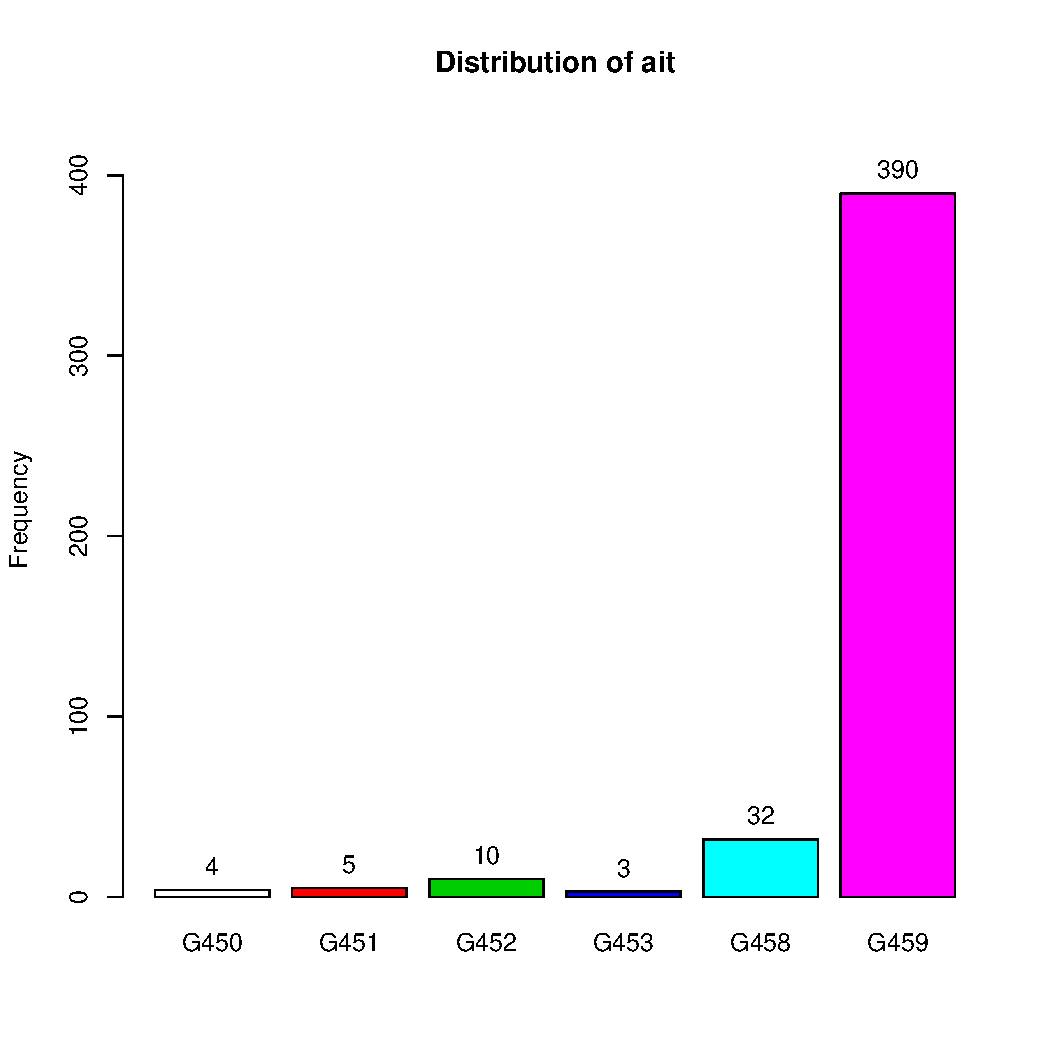
\includegraphics[width=\maxwidth]{figure/ait} 
\begin{kframe}\begin{verbatim}
## ait :  
##         Frequency Percent Cum. percent
## G450            4     0.8          0.8
## G451            5     1.0          1.8
## G452           12     2.4          4.2
## G453            4     0.8          5.1
## G458           35     7.1         12.1
## G459          435    87.9        100.0
##   Total       495   100.0        100.0
\end{verbatim}
\end{kframe}
\end{knitrout}


\section{Pneumonies}
\index{pneumonies}

\begin{knitrout}
\definecolor{shadecolor}{rgb}{0.969, 0.969, 0.969}\color{fgcolor}\begin{kframe}
\begin{verbatim}
## [1] "Pneumonies et AGE"
##    Min. 1st Qu.  Median    Mean 3rd Qu.    Max. 
##     0.0    62.0    77.0    70.9    85.0    98.0
\end{verbatim}
\end{kframe}
\end{knitrout}


Les pneumopaties bactériennes sans précision sont cotées J15.9 Dans la CIM10.
589 diagnostics de ce type ont été portés au SAU en 2013.

Les pneumonies bactériennes concernent les adultes agés des deux sexes. L'age moyen est de 70.9 ans et la moitié de ces patients ont 77 ans et plus.

\begin{knitrout}
\definecolor{shadecolor}{rgb}{0.969, 0.969, 0.969}\color{fgcolor}
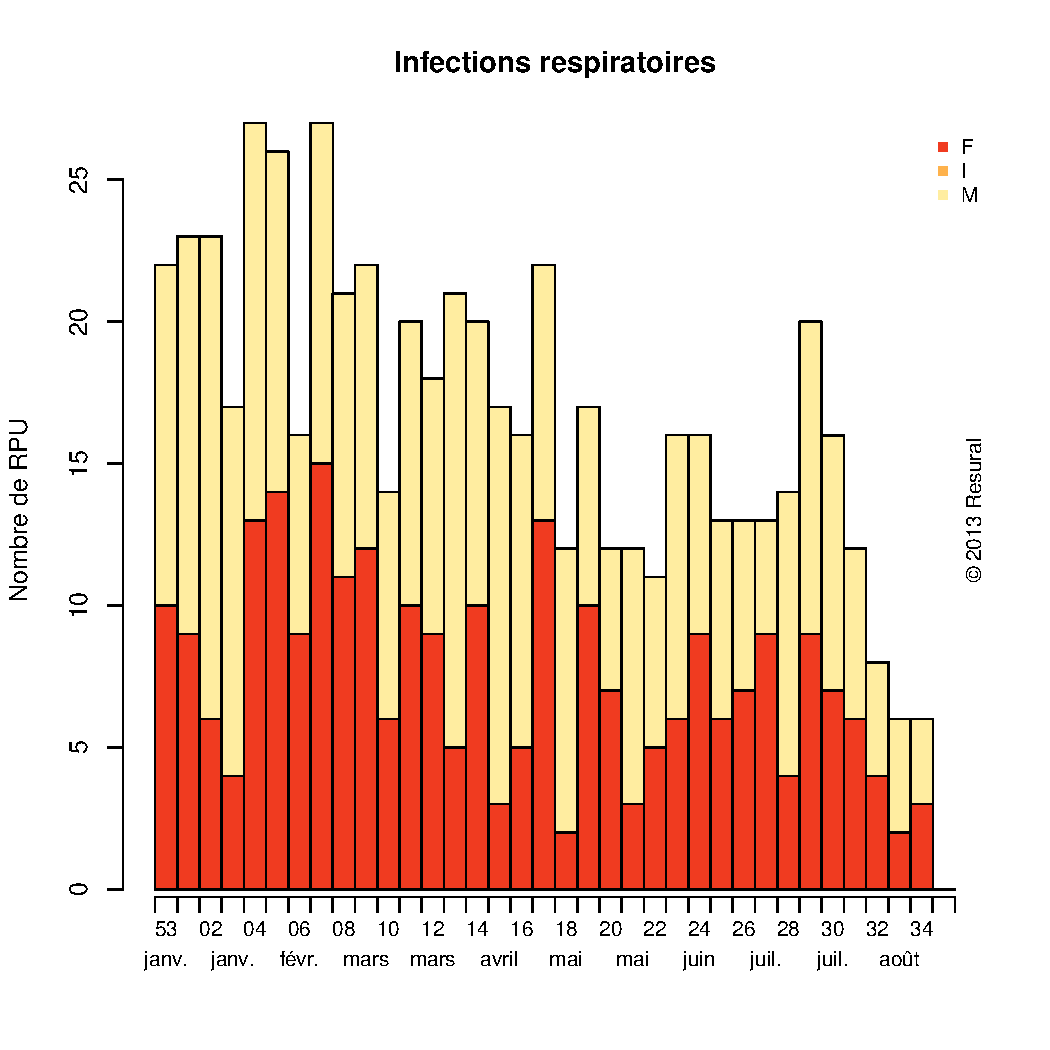
\includegraphics[width=\maxwidth]{figure/pneumo} 

\end{knitrout}


En fonction de la gravité (CCMU):
\begin{knitrout}
\definecolor{shadecolor}{rgb}{0.969, 0.969, 0.969}\color{fgcolor}\begin{kframe}
\begin{verbatim}
##    1    2    3    4    5    D    P NA's 
##   15  256  266   43    3    0    0    6
\end{verbatim}
\end{kframe}
\end{knitrout}


En fonction de la destination:
\begin{knitrout}
\definecolor{shadecolor}{rgb}{0.969, 0.969, 0.969}\color{fgcolor}\begin{kframe}
\begin{verbatim}
## integer(0)
\end{verbatim}
\end{kframe}
\end{knitrout}


En fonction de l'orientation:
\begin{knitrout}
\definecolor{shadecolor}{rgb}{0.969, 0.969, 0.969}\color{fgcolor}\begin{kframe}
\begin{verbatim}
##  CHIR FUGUE   HDT    HO   MED  OBST   PSA   REA   REO    SC  SCAM    SI 
##    10     0     0     0   189     0     0     4     0     4     0     2 
##  UHCD  NA's 
##   179   201
\end{verbatim}
\end{kframe}
\end{knitrout}


Deux patients porteurs de problèmes respiratoires sont orienté en chirurgie : erreur ou manque de place en médecine ?

\section{Syndrome grippal}
\index{syndrome grippal}

\begin{knitrout}
\definecolor{shadecolor}{rgb}{0.969, 0.969, 0.969}\color{fgcolor}
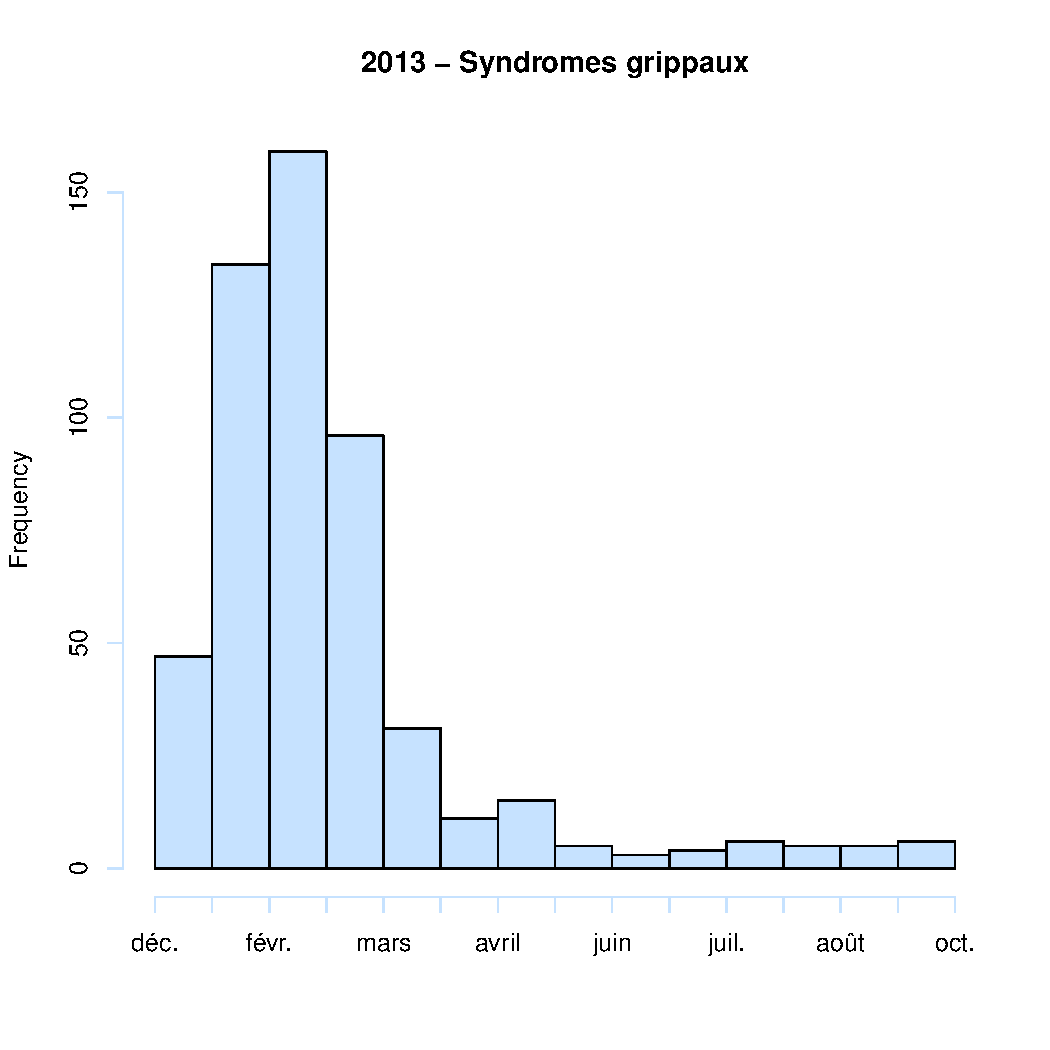
\includegraphics[width=\maxwidth]{figure/grippe} 

\end{knitrout}


\section{Malaises}
\index{malaise}

\begin{knitrout}
\definecolor{shadecolor}{rgb}{0.969, 0.969, 0.969}\color{fgcolor}
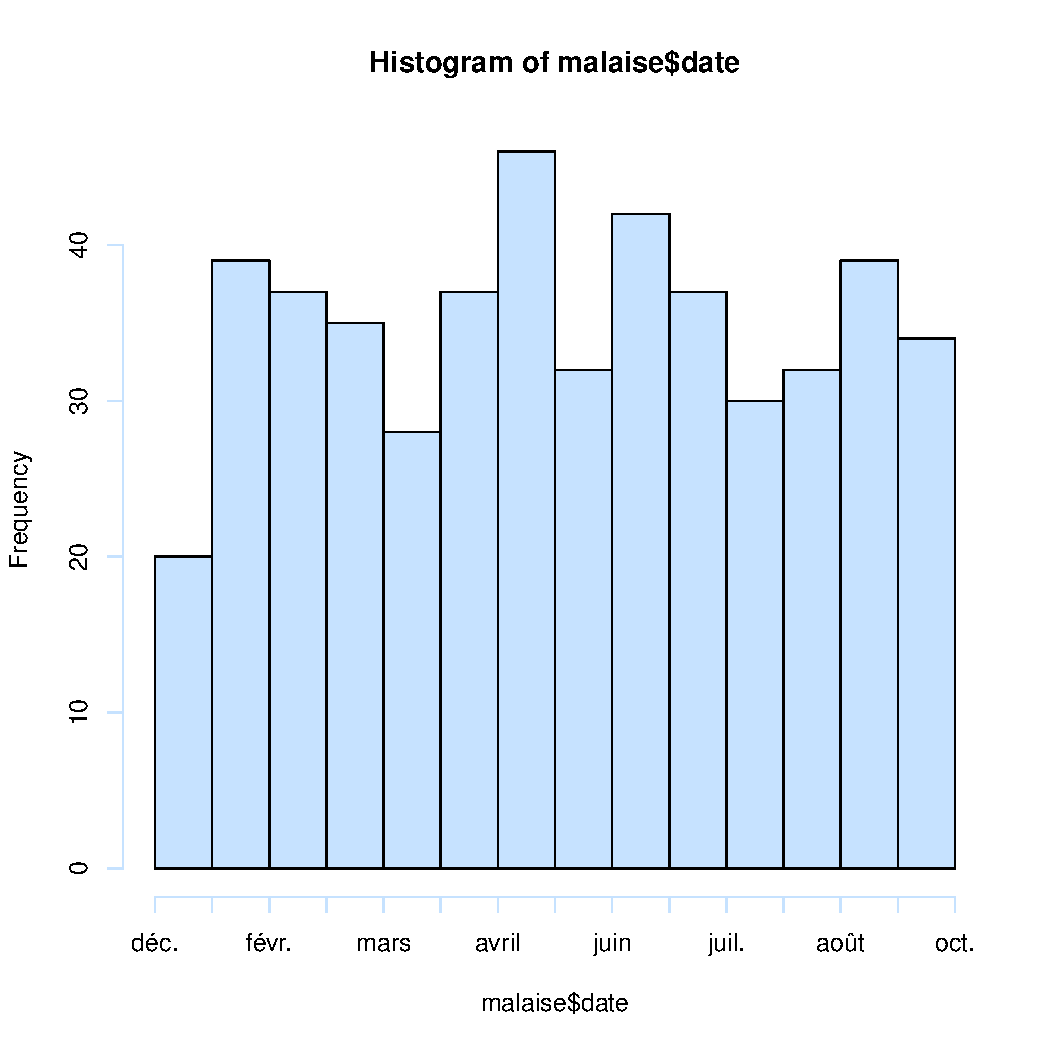
\includegraphics[width=\maxwidth]{figure/malaises} 

\end{knitrout}


malaise selon INVS (canicule):
\begin{knitrout}
\definecolor{shadecolor}{rgb}{0.969, 0.969, 0.969}\color{fgcolor}
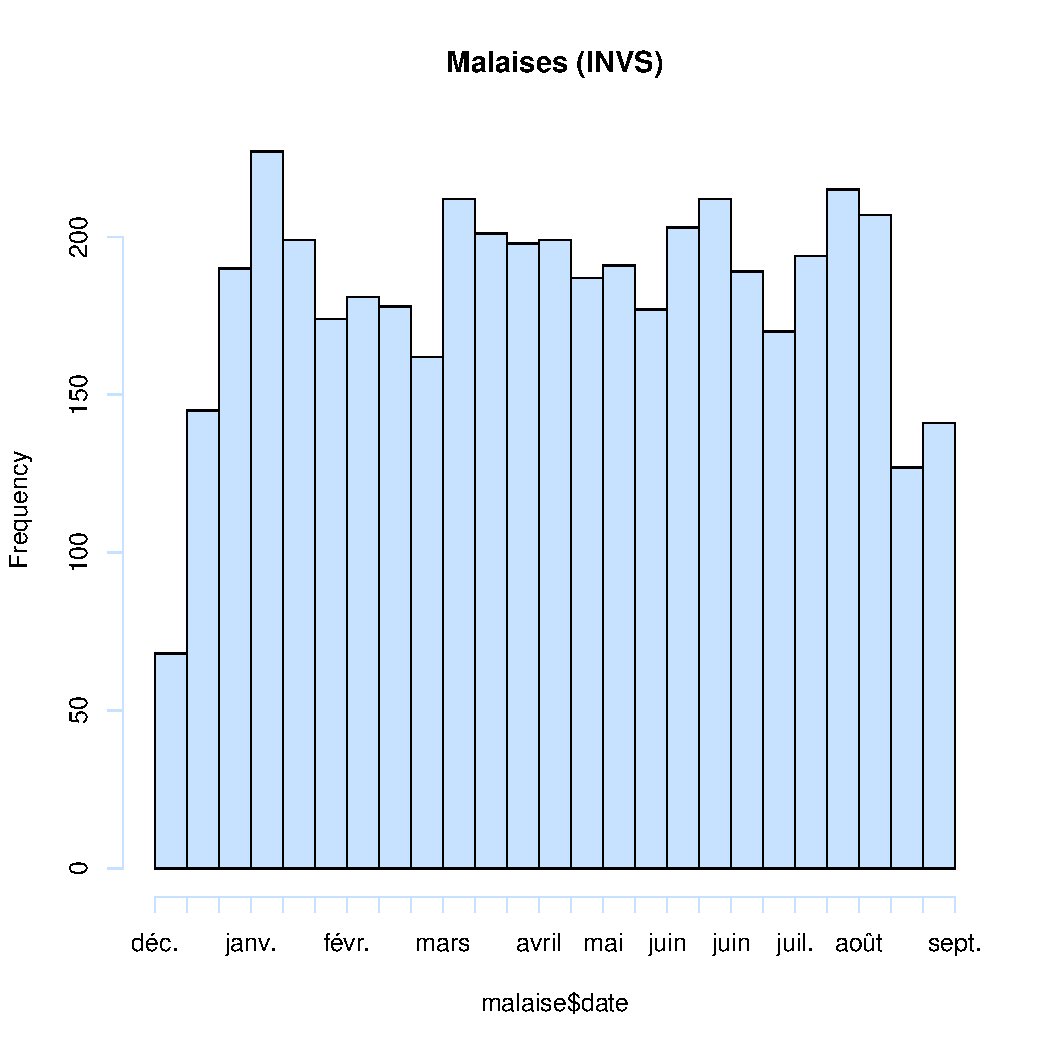
\includegraphics[width=\maxwidth]{figure/malaises_invs1} 

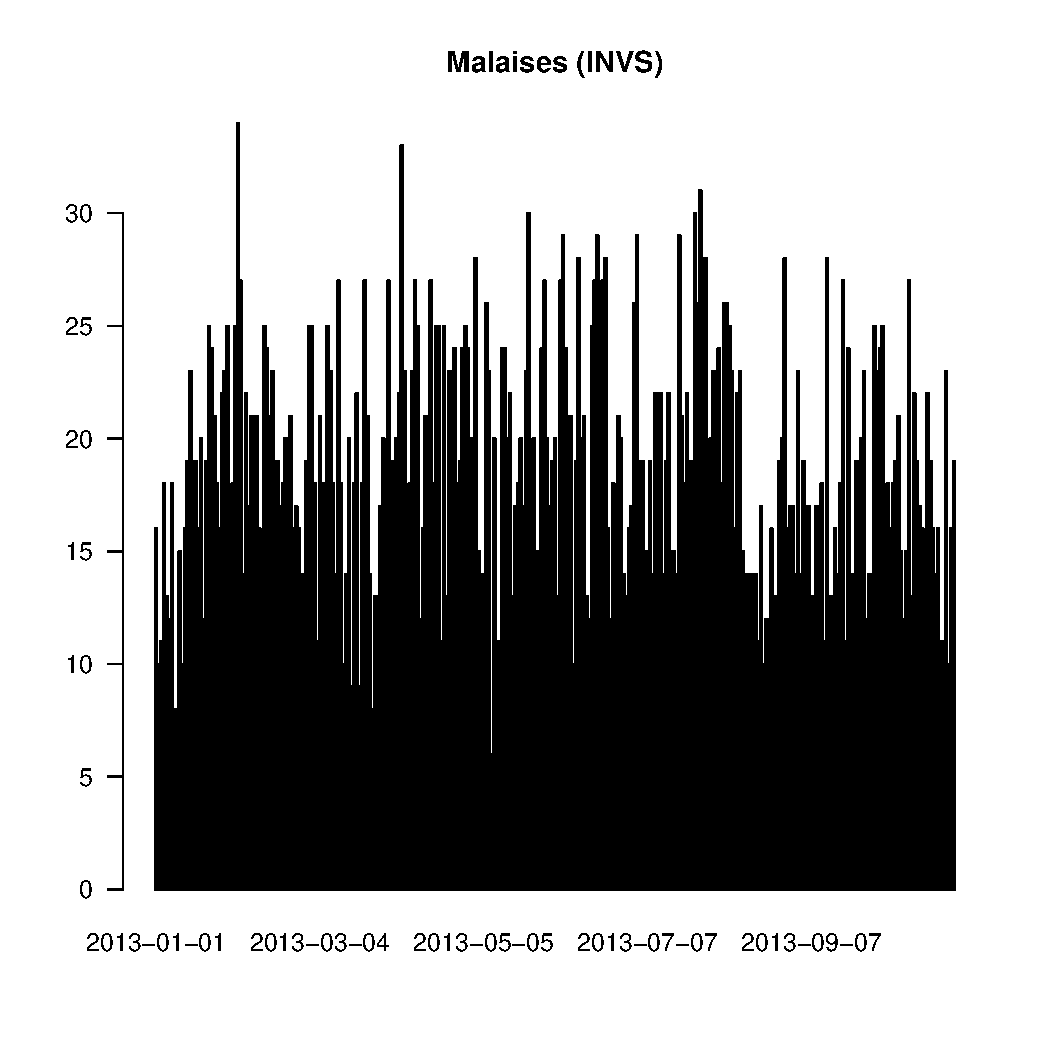
\includegraphics[width=\maxwidth]{figure/malaises_invs2} 

\end{knitrout}


\section{Marqueurs de canicule}
\index{Canicule@marqueurs}

Données hospitalières : nombre quotidien de passages dans des services d'urgence hospitaliers pour un diagnostic de malaise (codes Cim10 R42, R53 et R55), d'hyperthermie et autres effets directs de la chaleur (codes Cim10 T67 et X30), de déshydratation (code Cim10 E86) et d'hyponatrémie (code Cim10 E871)

- X30  Exposition à une chaleur naturelle excessive
- E86  Déplétion du volume du plasma ou du liquide extracellulaire, Déshydratation sauf choc hypovolémique

\begin{knitrout}
\definecolor{shadecolor}{rgb}{0.969, 0.969, 0.969}\color{fgcolor}
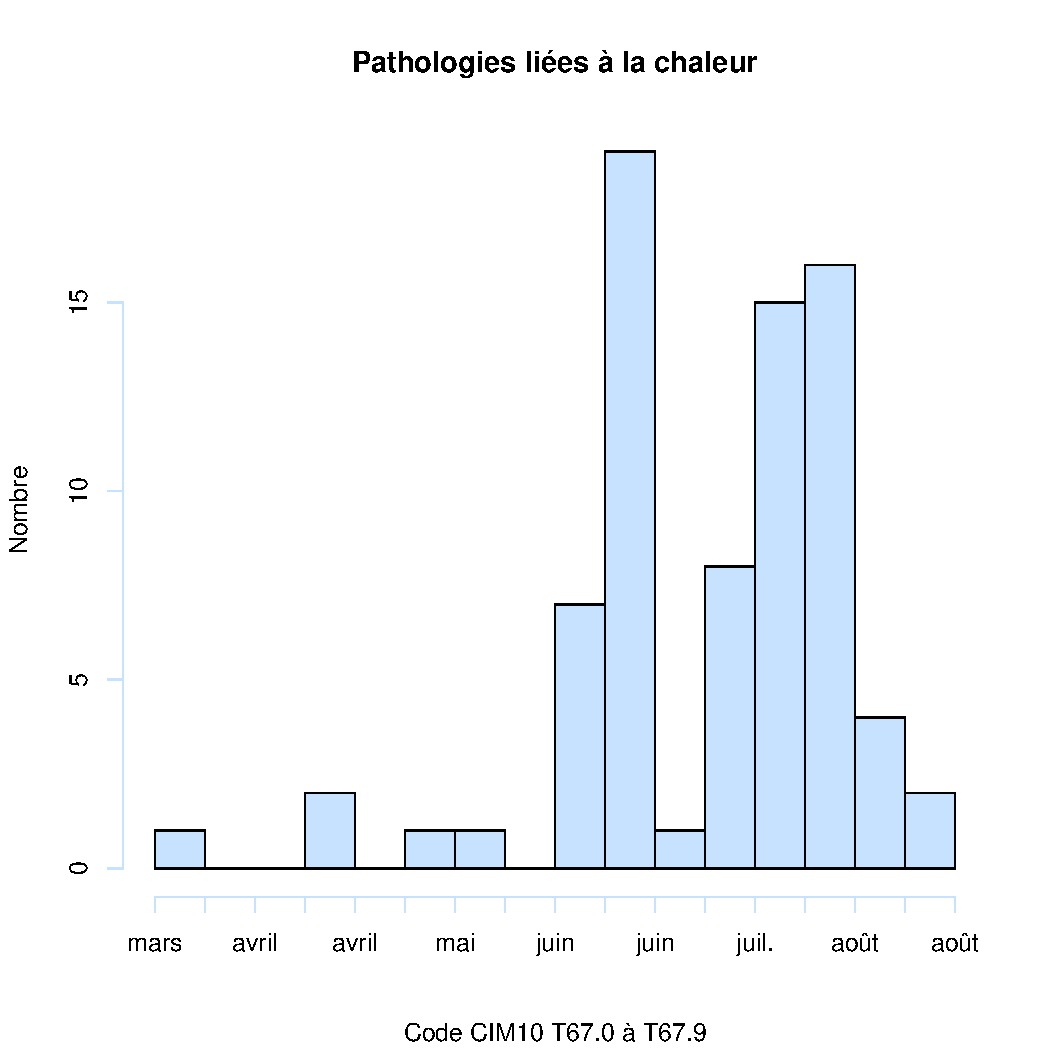
\includegraphics[width=\maxwidth]{figure/canicule1} 

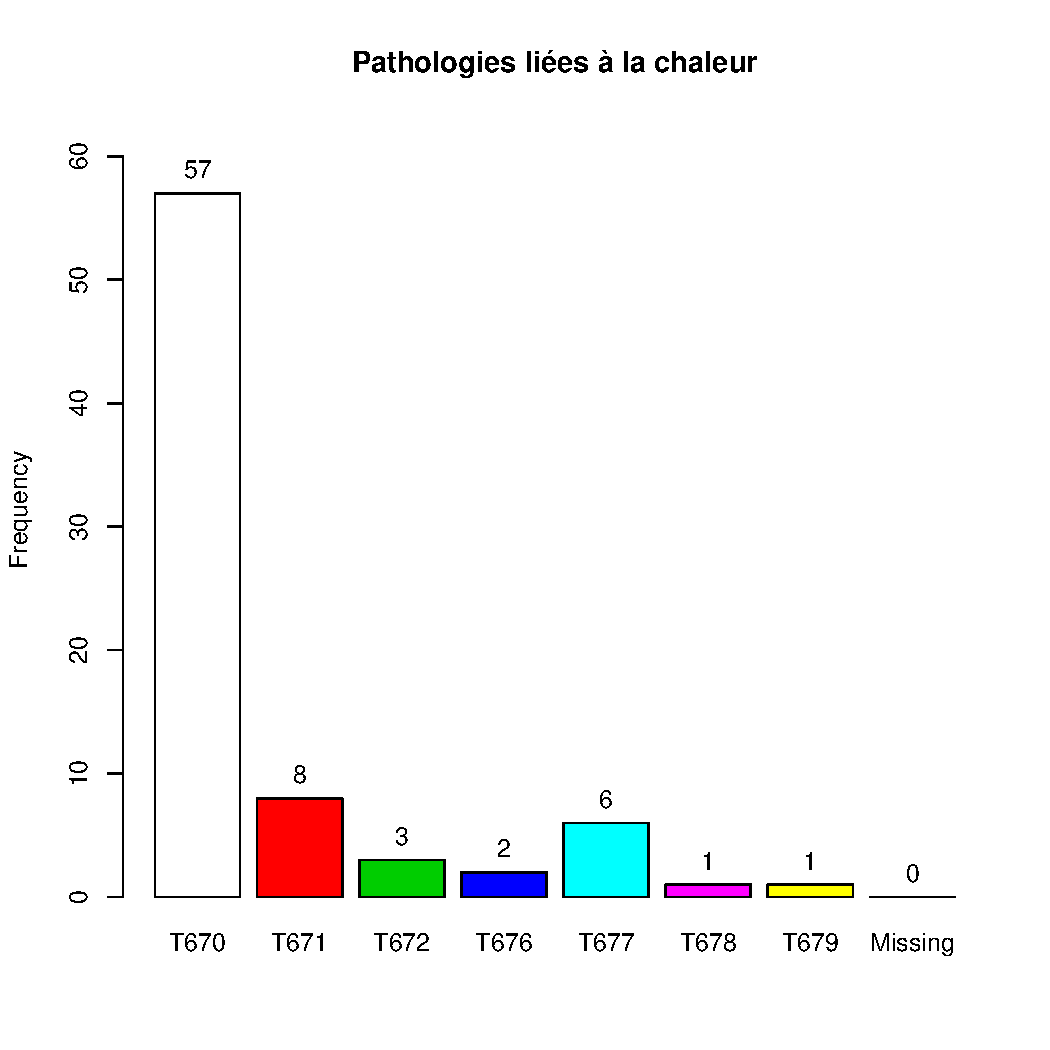
\includegraphics[width=\maxwidth]{figure/canicule2} 
\begin{kframe}\begin{verbatim}
## canicule$DP : 
##         Frequency Percent Cum. percent
## T670           56    72.7         72.7
## T671            8    10.4         83.1
## T672            3     3.9         87.0
## T676            2     2.6         89.6
## T677            6     7.8         97.4
## T678            1     1.3         98.7
## T679            1     1.3        100.0
##   Total        77   100.0        100.0
\end{verbatim}
\end{kframe}
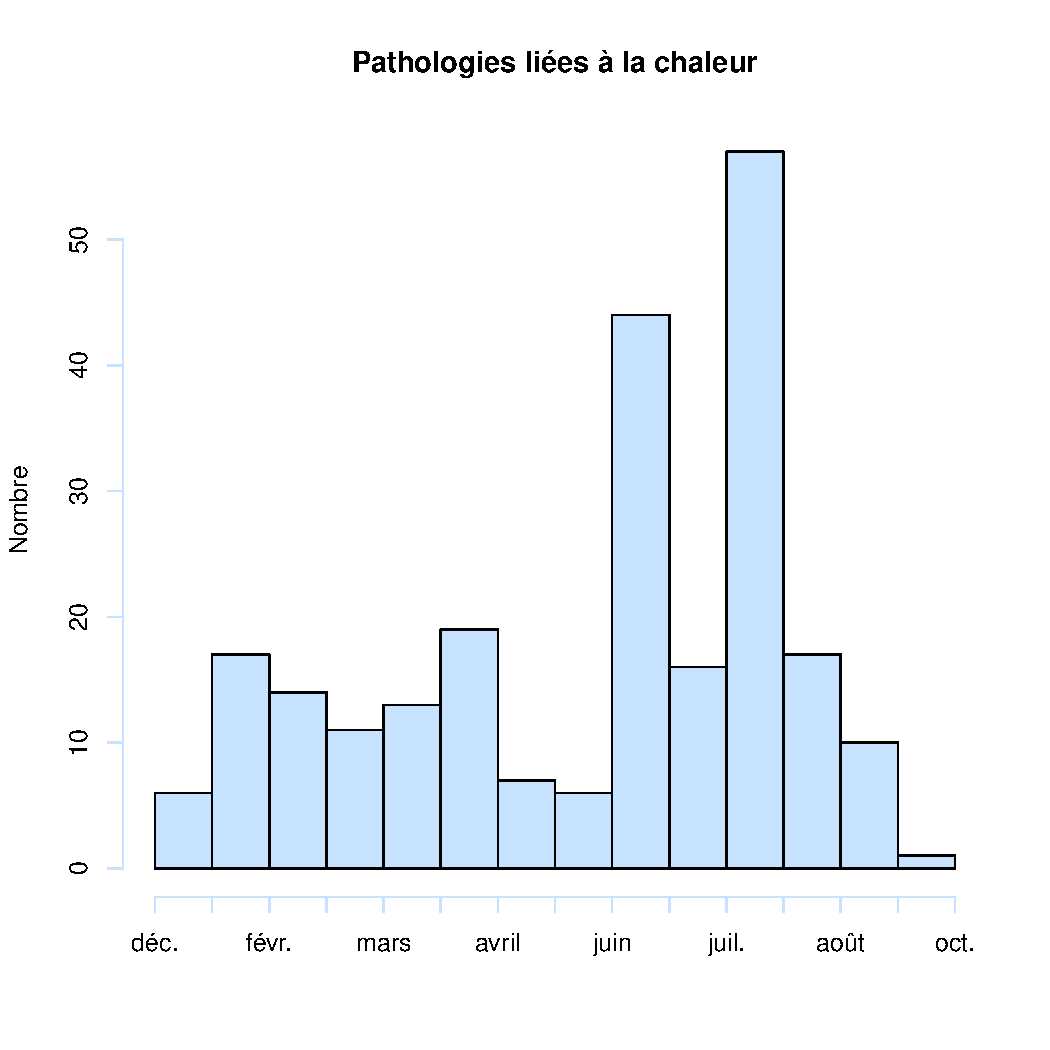
\includegraphics[width=\maxwidth]{figure/canicule3} 

\end{knitrout}



\chapter{Modalités de sortie}

% sortie.Rnw

\section{Mode de sortie}
\index{mode de sortie}

Le RPU connaît trois mode de sortie des urgences:
\begin{enumerate}
  \item le décès: le patient est déclaré décédé aux urgences.
  \item le retour à domicile ou ce qui en tient lieu (y compris la voie publique)
  \item l'hospitalisation (mutation ou transfert)
  \begin{itemize}
  \item mutation: le patient est hospitalisé dans une autre unité médicale de la même entité juridique sauf pour les établissements privés visés aux alinéas d et e de l'article L162-22-6 du code de la sécurité sociale.
  \item transfert: le patient est hospitalisé dans une autre  entité juridique sauf pour les établissements privés visés aux alinéas d et e de l'article L162-22-6 du code de la sécurité sociale.
\end{itemize}
\end{enumerate}

% Mode de SORTIE.png: 669x437 pixel, 72dpi, 23.60x15.42 cm, bb=0 0 669 437
 \begin{figure}[h]
 \centering
 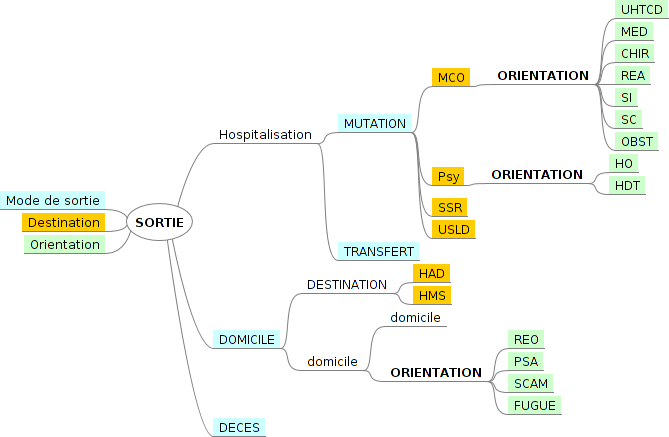
\includegraphics[width=9cm,height=7cm,bb=0 0 669 437]{figure/Mode de SORTIE.png}
 \caption{Modes de sortie}
\end{figure}

% latex table generated in R 2.15.1 by xtable 1.7-1 package
% Wed Sep 18 09:03:56 2013
\begin{table}[ht]
\centering
\begin{tabular}{|l|r|r|}
  \hline
 & n & \% \\ 
  \hline
Décès & 2 & 0.00 \\ 
  Domicile & 142443 & 64.06 \\ 
  Mutation & 43781 & 19.69 \\ 
  $<$NA$>$ & 32921 & 14.81 \\ 
  Transfert & 3204 & 1.44 \\ 
   \hline
\end{tabular}
\caption[Mode de sortie des urgences]{Mode de sortie des urgences. <NA> est le nombre de non réponses à cet item} 
\label{tab.sortie}
\end{table}



\section{Mode de sortie selon la structure}

Les données par établissement sont résumées dans le tableau \ref{tab.sortie_etab} page \pageref{tab.sortie_etab}

% latex table generated in R 2.15.1 by xtable 1.7-1 package
% Wed Sep 18 09:03:56 2013
\begin{table}[ht]
\centering
\begin{tabular}{|l|r|r|r|r|r|r|}
  \hline
 & Décès & Domicile & Mutation & $<$NA$>$ & Transfert & Sum \\ 
  \hline
3Fr & 0.00 & 90.38 & 1.80 & 7.65 & 0.16 & 99.99 \\ 
  Alk & 0.00 & 81.88 & 13.84 & 1.58 & 2.70 & 100.00 \\ 
  Col & 0.00 & 73.21 & 22.82 & 2.08 & 1.90 & 100.01 \\ 
  Dia & 0.00 & 82.99 & 9.27 & 7.21 & 0.53 & 100.00 \\ 
  Geb & 0.00 & 39.86 & 0.92 & 58.70 & 0.51 & 99.99 \\ 
  Hag & 0.00 & 56.95 & 24.14 & 14.43 & 4.49 & 100.01 \\ 
  Hus & 0.00 & 2.76 & 54.31 & 42.92 & 0.00 & 99.99 \\ 
  Mul & 0.00 & 61.97 & 14.00 & 23.79 & 0.25 & 100.01 \\ 
  Odi & 0.00 & 93.29 & 0.00 & 2.15 & 4.56 & 100.00 \\ 
  Sel & 0.01 & 79.02 & 20.96 & 0.01 & 0.00 & 100.00 \\ 
  Wis & 0.00 & 76.26 & 21.79 & 0.75 & 1.20 & 100.00 \\ 
  Sav & 0.00 & 72.81 & 19.01 & 7.10 & 1.08 & 100.00 \\ 
   \hline
\end{tabular}
\caption[Mode de sortie selon l'établissement]{Mode de sortie des urgences selon l'établissement (en pourcentage). <NA> est le nombre de non réponses à cet item} 
\label{tab.sortie_etab}
\end{table}




\section{Orientation}
\index{orientation}

Le mode de sortie est affiné par la rubrique ORIENTATION avec la ventilation suivante:

\begin{itemize}
  \item NA:    Pas d'informations
  \item MCO:		Hospitalisation conventionnelle
  \item SSR:		Soins de suite et de réadaptation
  \item SLD:		Soins de longue durée
  \item PSY: 		Psychiatrie
  \item HAD:		Hospitalisation à domicile
  \item HMS:		Hébergement médico-social
\end{itemize}

On notera que le retour à domicile proprement dit ne figure pas parmi les items et cette modalité est implicite. On peut supposer que les NA's correspondent à cette modalité. Cependant une ambiguité demeure car les non réponses sont aussi représentées par ce symbole.

\begin{knitrout}
\definecolor{shadecolor}{rgb}{0.969, 0.969, 0.969}\color{fgcolor}\begin{kframe}
\begin{alltt}
\hlcom{# drop.levels permet d'éliminer le level 0 qui est nul}
a <- \hlkwd{drop.levels}(d1$ORIENTATION)
\hlkwd{summary}(a)
\end{alltt}
\begin{verbatim}
##   CHIR  FUGUE    HDT     HO    MED   OBST    PSA    REA    REO     SC 
##   4989    172     89     21  11231     64   2058    664    967    898 
##   SCAM     SI   UHCD   NA's 
##    331    920  22047 177900
\end{verbatim}
\begin{alltt}

\hlkwd{table}(a, useNA = \hlstr{"always"})
\end{alltt}
\begin{verbatim}
## a
##   CHIR  FUGUE    HDT     HO    MED   OBST    PSA    REA    REO     SC 
##   4989    172     89     21  11231     64   2058    664    967    898 
##   SCAM     SI   UHCD   <NA> 
##    331    920  22047 177900
\end{verbatim}
\begin{alltt}

\hlkwd{table}(d1$DESTINATION, d1$GRAVITE)
\end{alltt}
\begin{verbatim}
##      
##           1     2     3     4     5     D     P
##   NA      0     0     0     0     0     0     0
##   MCO  1681 18002 17988  1858   475     6    97
##   SSR     0    34    20     2     0     0     0
##   SLD     0     6     2     2     0     0     0
##   PSY    34   194   115    10     5     0   422
##   HAD     0     1     0     0     0     0     0
##   HMS     3    12     2     0     0     0     0
\end{verbatim}
\end{kframe}
\end{knitrout}


\section{Destination}
\index{destination}
% latex table generated in R 2.15.1 by xtable 1.7-1 package
% Wed Sep 18 09:03:57 2013
\begin{table}[ht]
\centering
\begin{tabular}{rr}
  \hline
 & \% \\ 
  \hline
HAD & 0.00 \\ 
  HMS & 0.04 \\ 
  MCO & 98.10 \\ 
  PSY & 1.72 \\ 
  SLD & 0.02 \\ 
  SSR & 0.12 \\ 
   \hline
\end{tabular}
\caption{Destination des patients non rentrés à domicile après leur passage aux urgences} 
\label{tab.dest.hosp}
\end{table}
% latex table generated in R 2.15.1 by xtable 1.7-1 package
% Wed Sep 18 09:03:57 2013
\begin{table}[ht]
\centering
\begin{tabular}{rr}
  \hline
 & \% \\ 
  \hline
DOM & 78.90 \\ 
  HAD & 0.00 \\ 
  HMS & 0.01 \\ 
  MCO & 20.70 \\ 
  PSY & 0.36 \\ 
  SLD & 0.00 \\ 
  SSR & 0.03 \\ 
   \hline
\end{tabular}
\caption{Devenir des patients à la sortie des urgences. DOM représentent ceux qui sont repartis vers leur domicile ou ce qui en tient lieu (sous l'hypothèse que toutes les non réponses correspondent à un retour à domicile).} 
\label{tab.dest}
\end{table}



\section{Incohérences}
\ref{sortie:erreurs}
On isole le groupe "mode de sortie = domicile) et on relève les résultats de l'item "orientation":
\begin{knitrout}
\definecolor{shadecolor}{rgb}{0.969, 0.969, 0.969}\color{fgcolor}\begin{kframe}
\begin{alltt}
a <- d1[d1$MODE_SORTIE == \hlstr{"Domicile"}, ]
\hlkwd{summary}(\hlkwd{as.factor}(a$ORIENTATION))
\end{alltt}
\begin{verbatim}
##   CHIR  FUGUE    HDT     HO    MED   OBST    PSA    REA    REO     SC 
##     83    171     10      2     50      1   2017      9    945      3 
##   SCAM     SI   UHCD   NA's 
##    331     21    169 171552
\end{verbatim}
\begin{alltt}
t <- \hlkwd{table}(\hlkwd{as.factor}(a$ORIENTATION))
\hlkwd{round}(\hlkwd{prop.table}(t) * 100, 2)
\end{alltt}
\begin{verbatim}
## 
##  CHIR FUGUE   HDT    HO   MED  OBST   PSA   REA   REO    SC  SCAM    SI 
##  2.18  4.49  0.26  0.05  1.31  0.03 52.91  0.24 24.79  0.08  8.68  0.55 
##  UHCD 
##  4.43
\end{verbatim}
\begin{alltt}
\hlkwd{tab1}(\hlkwd{as.factor}(a$ORIENTATION), sort.group = \hlstr{"decreasing"}, horiz = TRUE, cex.names = 0.8, 
    xlab = \hlstr{""}, main = \hlstr{"Orientation des patients non hospitalisés"}, missing = F)
\end{alltt}
\end{kframe}
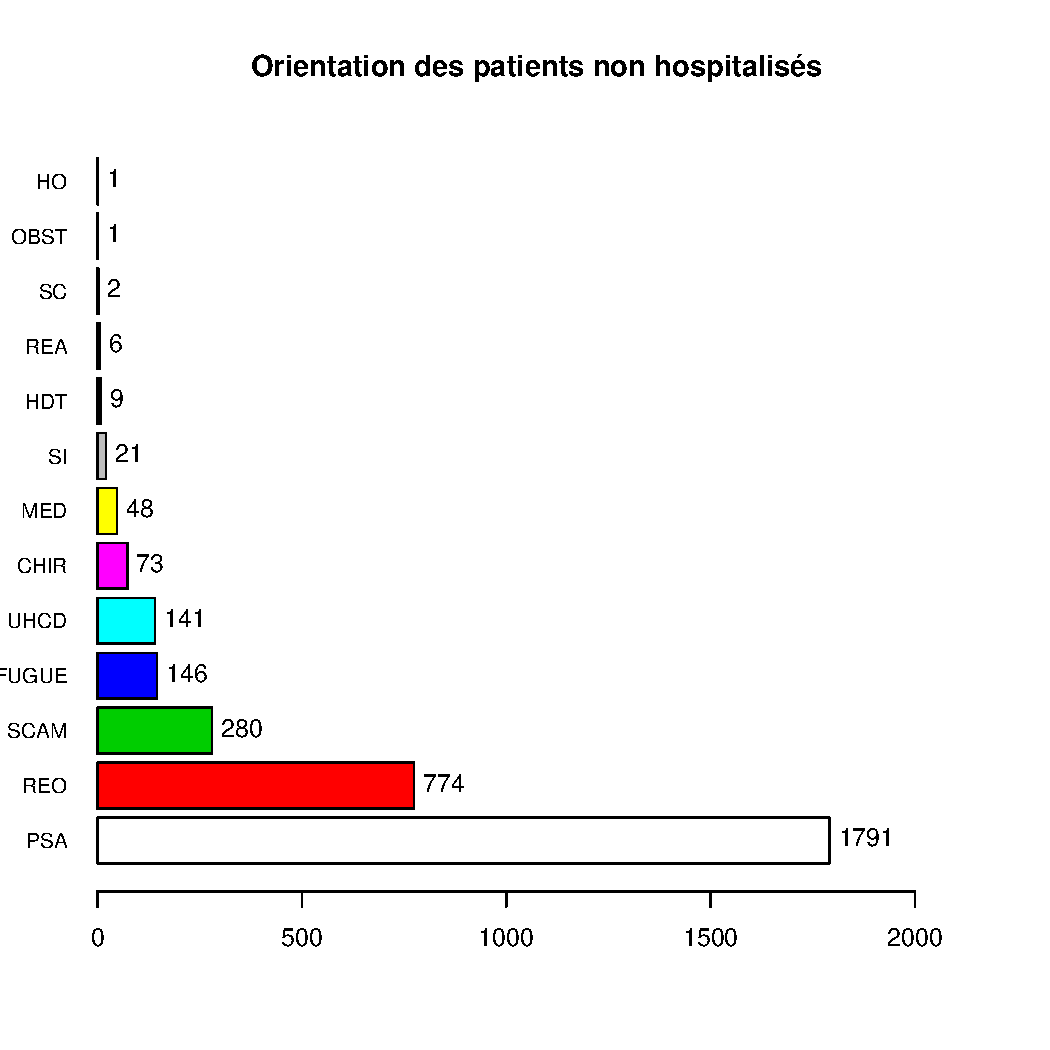
\includegraphics[width=\maxwidth]{figure/fausses_sorties} 
\begin{kframe}\begin{verbatim}
## as.factor(a$ORIENTATION) : 
##         Frequency   %(NA+)   %(NA-)
## NA's       171552     97.8      0.0
## PSA          2017      1.2     52.9
## REO           945      0.5     24.8
## SCAM          331      0.2      8.7
## FUGUE         171      0.1      4.5
## UHCD          169      0.1      4.4
## CHIR           83      0.0      2.2
## MED            50      0.0      1.3
## SI             21      0.0      0.6
## HDT            10      0.0      0.3
## REA             9      0.0      0.2
## SC              3      0.0      0.1
## HO              2      0.0      0.1
## OBST            1      0.0      0.0
##   Total    175364    100.0    100.0
\end{verbatim}
\end{kframe}
\end{knitrout}

Certaines orientations sont incompatibles avec une non hospitalisation:
\begin{itemize}
  \item HO
  \item Obstétrique
  \item Soins continus, soins intensifs et réanimation
  \item UHCD, médecine et chirurgie
  
\end{itemize}




\chapter{Modalités d'orientation}

% orientation.Rnw

\index{orientation}

Le mode d'orientation au sens du RPU est une rubrique un peu fourre-tout regrouppant des hospitalisations comme des sorties "anormales" de la filère de soins (fugues, sotie contre avis, etc.).


\chapter{Courbes d'activité régionale}

% activite_su.Rnw
% Courbe d'activité régionale
\index{Activité régionale}
 
%note\footnote{activite_su_Rnw}

\section{Variation du nombre total de passages journaliers}
\index{Passages@journaliers}


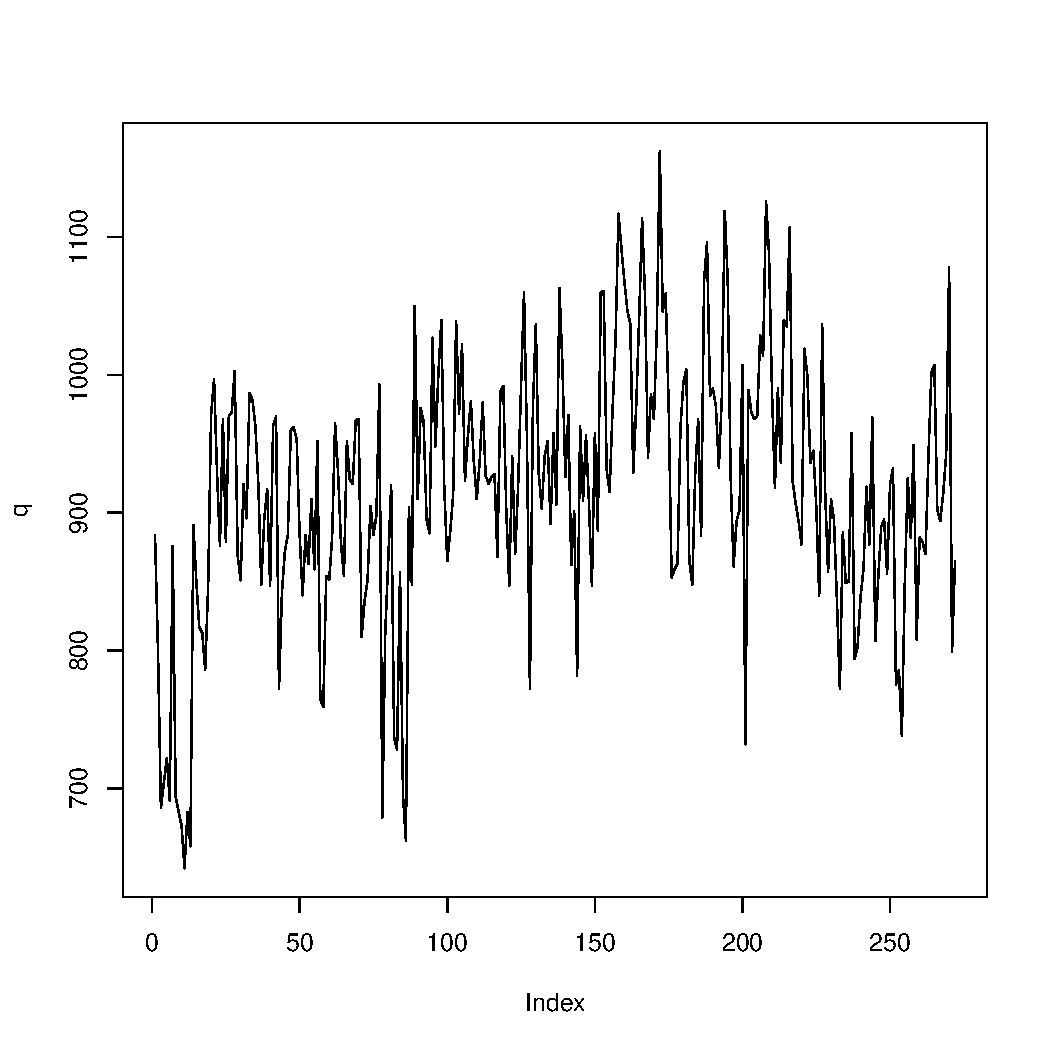
\includegraphics[width=\maxwidth]{figure/passages_totaux1} 
% latex table generated in R 2.15.1 by xtable 1.7-1 package
% Wed Sep 18 09:03:59 2013
\begin{table}[ht]
\centering
\begin{tabular}{rrrrrrrrr}
  \hline
 & n & Min & Q25 & Moyenne & E-type & Médiane & Q75 & Max \\ 
  \hline
 & 242.00 & 642.00 & 863.50 & 918.80 & 96.80 & 922.00 & 977.00 & 1162.00 \\ 
   \hline
\end{tabular}
\caption[Passages totaux]{Passages totaux} 
\label{tab:pt}
\end{table}

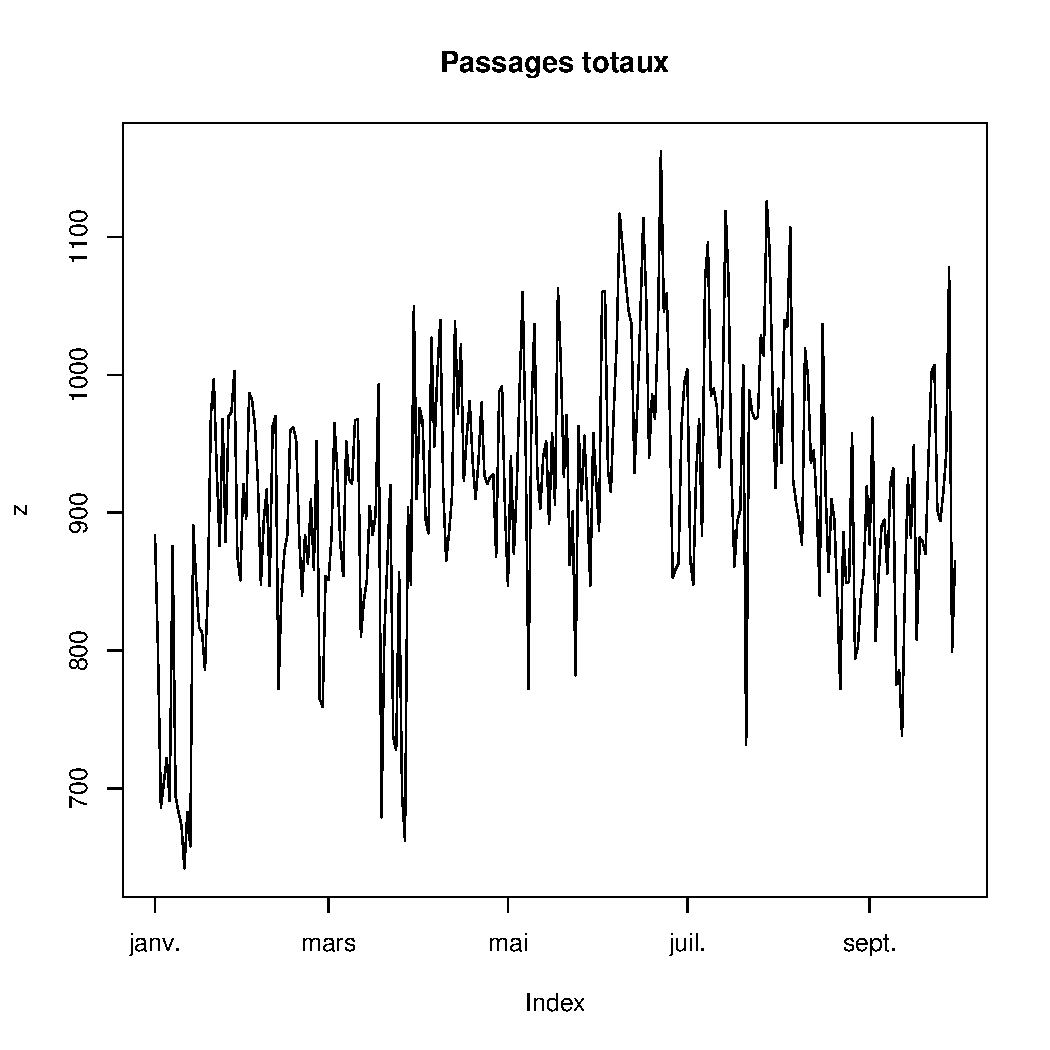
\includegraphics[width=\maxwidth]{figure/passages_totaux2} 

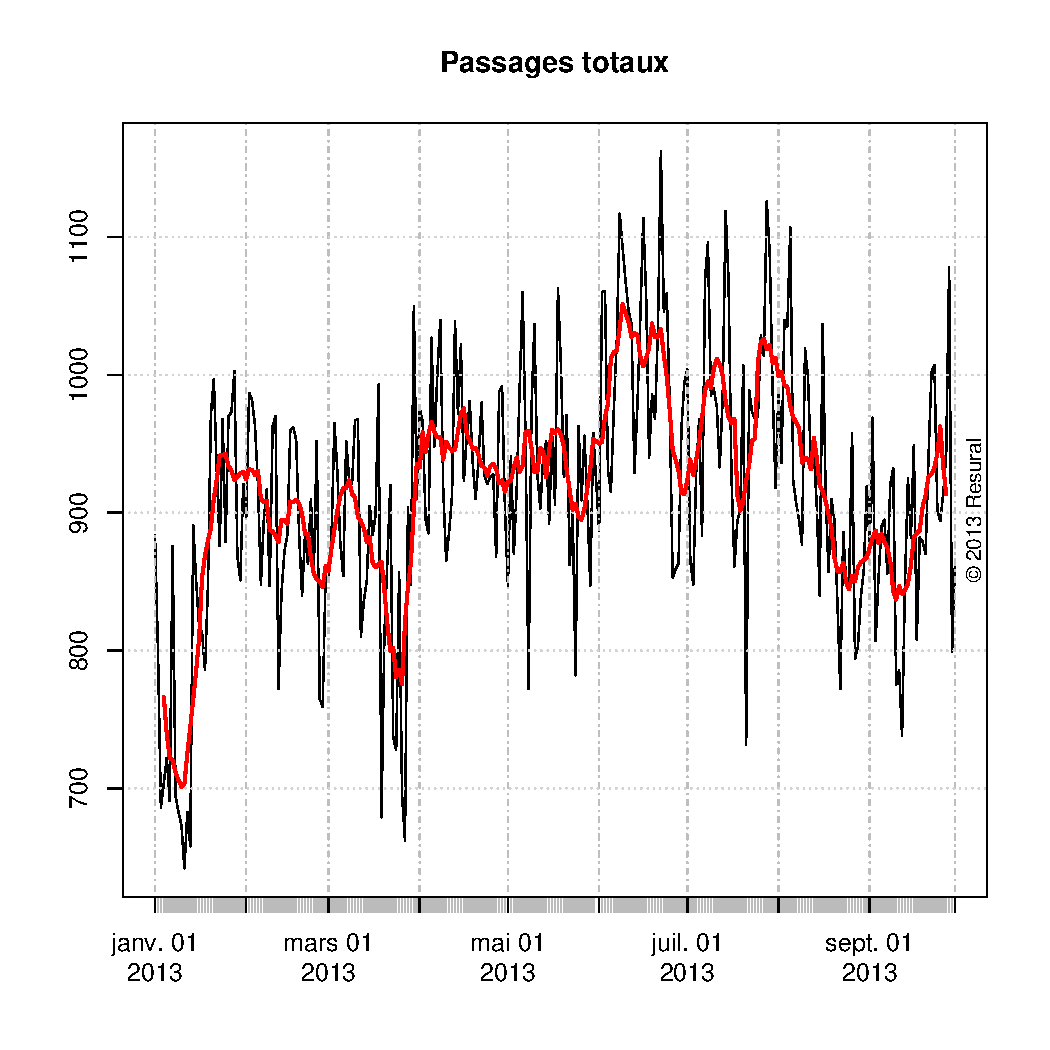
\includegraphics[width=\maxwidth]{figure/passages_totaux3} 




\section{Variation du pourcentage journalier de retour à domicile}
\index{Retour à domicile}

Le nombre de retours à domicile est obtenu à partir de la rubrique MODE\_SORTIE. Il s'agit en fait des patients qui n'ont pas été hospitalisés. Sont également comptabilisé dans cette rubrique les sorties atypiques.

Les variation du retour journalier à domicile sont calculés de la manière suivante:
\begin{description}
  \item[numérateur] somme quotidienne où MODE\_SORTIE == Domicile
  \item[dénominateur] somme quotidienne des ENTREE (correspond à q)
\end{description}

% latex table generated in R 2.15.1 by xtable 1.7-1 package
% Wed Sep 18 09:04:02 2013
\begin{table}[ht]
\centering
\begin{tabular}{rrrrrrrrr}
  \hline
 & n & Min & Q25 & Moyenne & E-type & Médiane & Q75 & Max \\ 
  \hline
 & 242.00 & 0.60 & 0.60 & 0.60 & 0.00 & 0.60 & 0.70 & 0.80 \\ 
   \hline
\end{tabular}
\caption[Retour à domicile]{Retours à domicile - patients n'ayant été ni hospitalisés, ni transférés dans un autre établissement. Ce taux est plus faible en début d'année, lorsque les épisodes de tension sont plus fréquents.} 
\label{tab:rd}
\end{table}

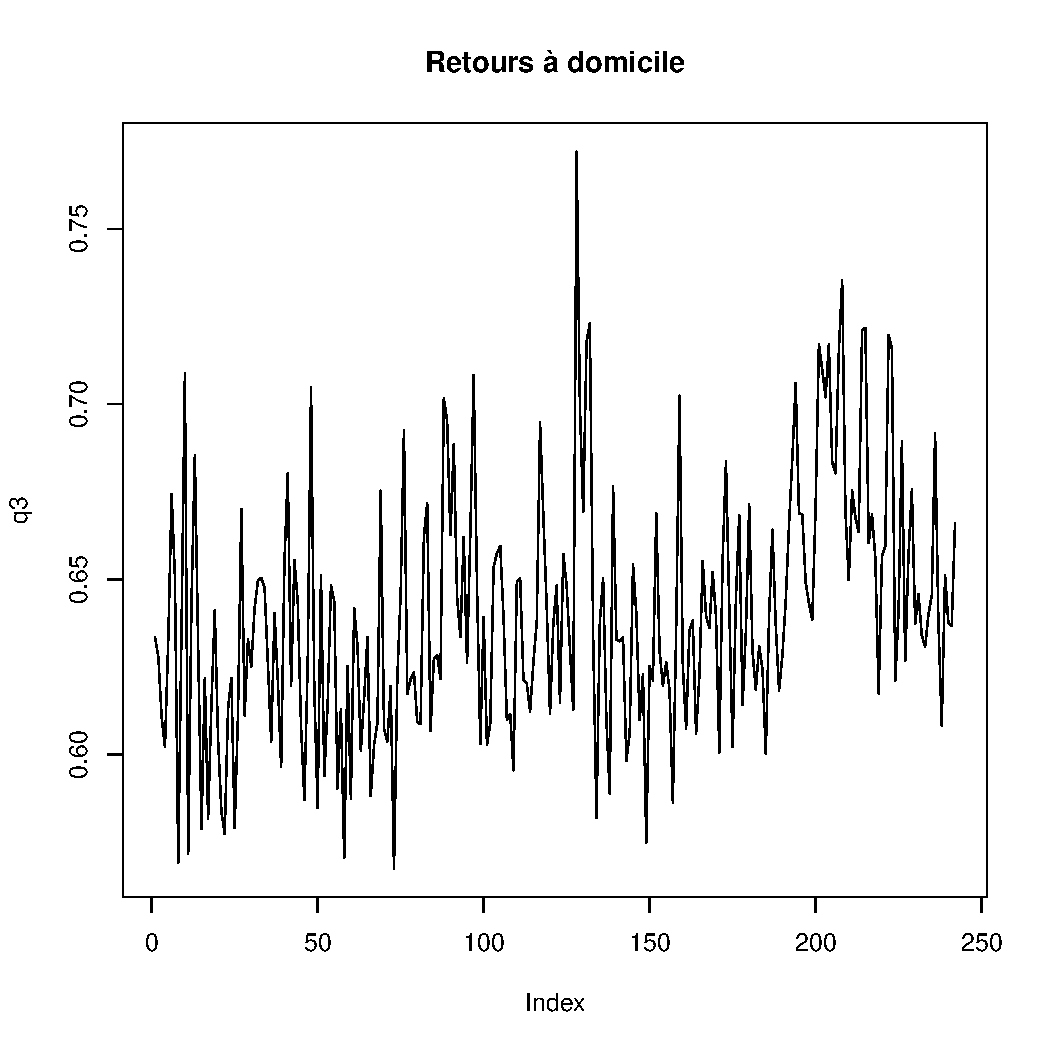
\includegraphics[width=\maxwidth]{figure/retour_dom} 



On refait le calcul de q en tenant compte des non réponses:

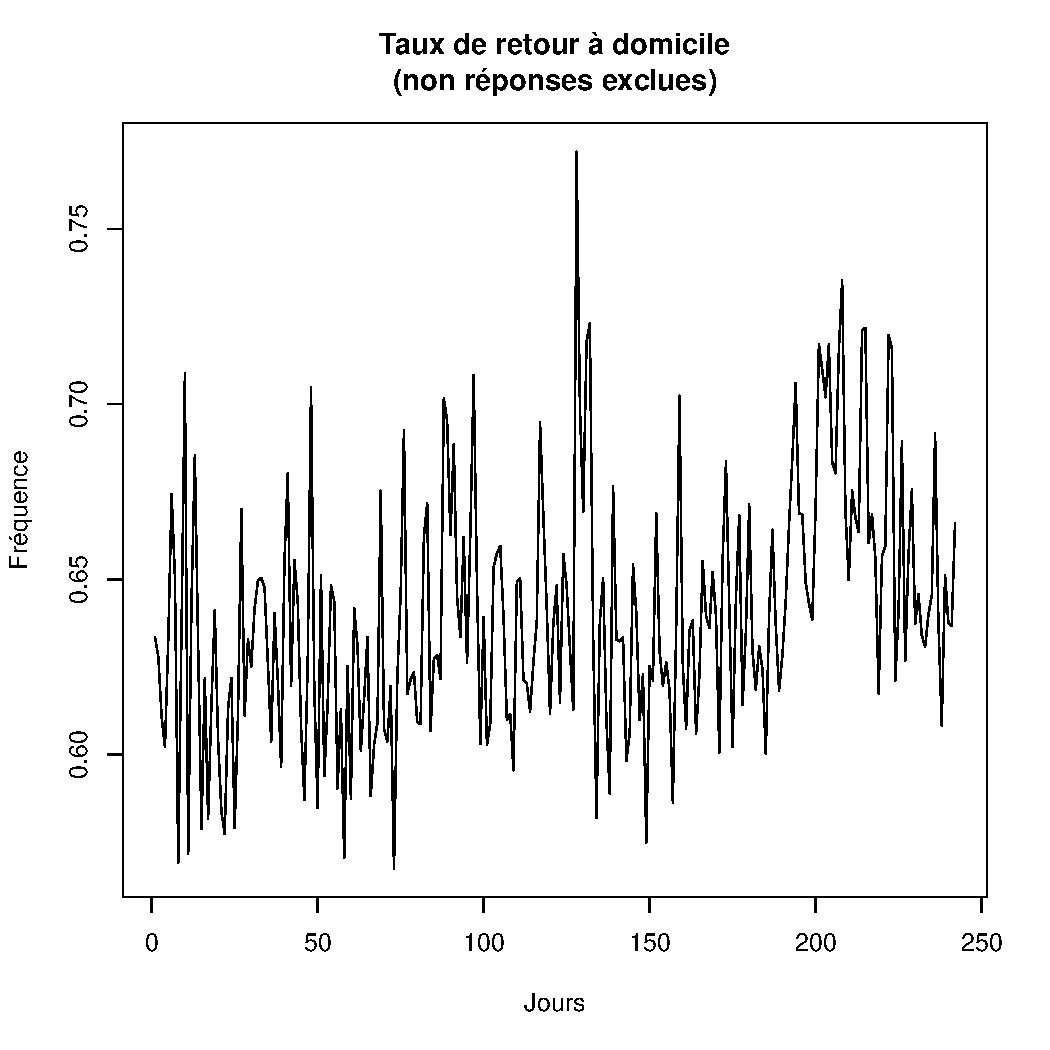
\includegraphics[width=\maxwidth]{figure/retour_dom2} 



Si on considère que tout ce qui n'est pas un retour à domicile constitue une hospitalisation, on peut tracer un graphique, miroir du précédent. La ligne bleue représente la moyenne lissée sur sept jours. On notera le taux d'hospitalisation élévé du début de l'année, correspondant à une période de forte tension. Les fluctuations de ce paramètre (comme le retour à domicile) est une piste intéressante dans le cadre de la recherche d'indicateurs d'hôpital en tension, cependant les seuils d'alerte (triggers) restent à déterminer.

% latex table generated in R 2.15.1 by xtable 1.7-1 package
% Wed Sep 18 09:04:04 2013
\begin{table}[ht]
\centering
\begin{tabular}{rrrrrrrrr}
  \hline
 & n & Min & Q25 & Moyenne & E-type & Médiane & Q75 & Max \\ 
  \hline
 & 242.00 & 0.20 & 0.20 & 0.20 & 0.00 & 0.30 & 0.30 & 0.30 \\ 
   \hline
\end{tabular}
\caption[Hospitalisations]{Hospitalisations (ou transferts) sans les non réponses} 
\label{tab:hosp}
\end{table}
   n Min Q25 Moyenne E-type Médiane Q75 Max
 242 0.2 0.2     0.2      0     0.3 0.3 0.3

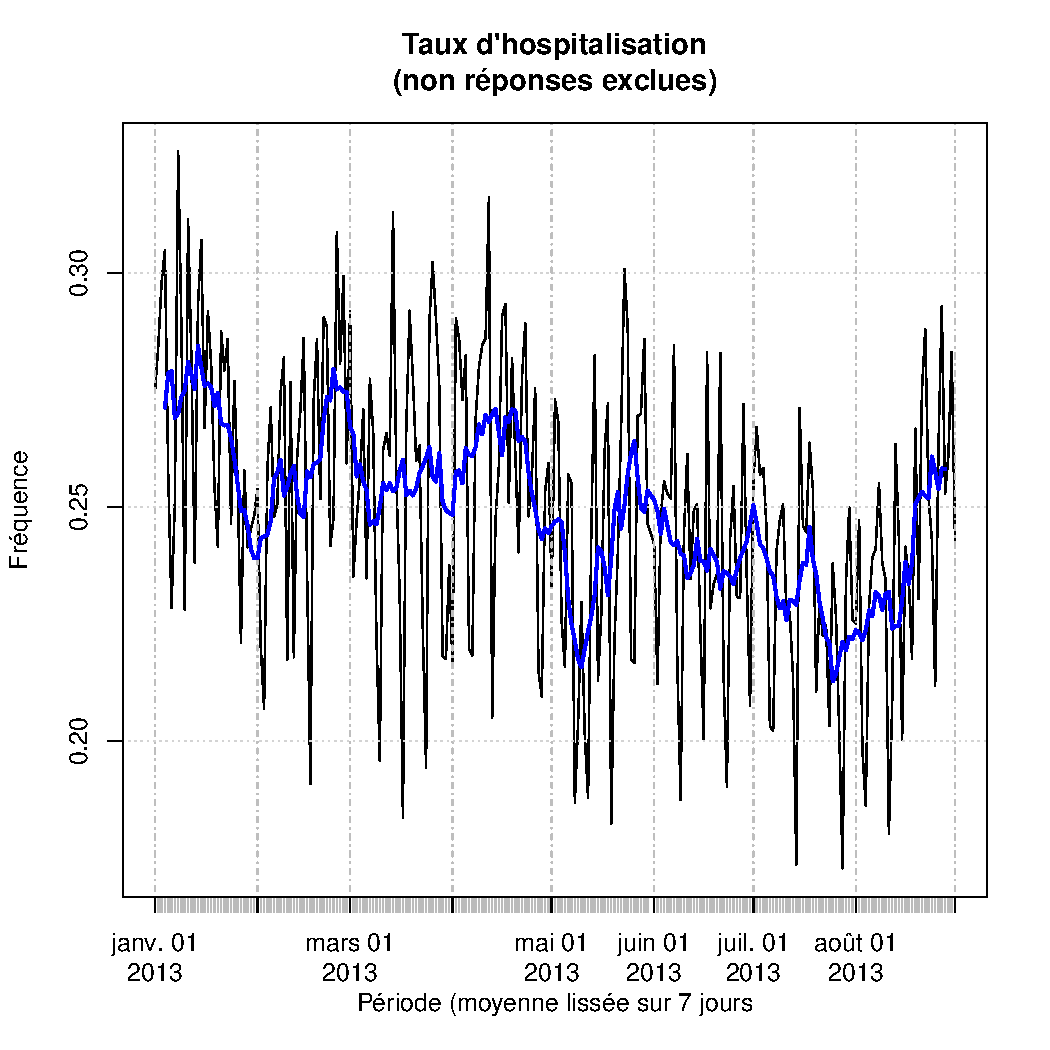
\includegraphics[width=\maxwidth]{figure/hospit} 




Le taux de réponse pour cet item est de

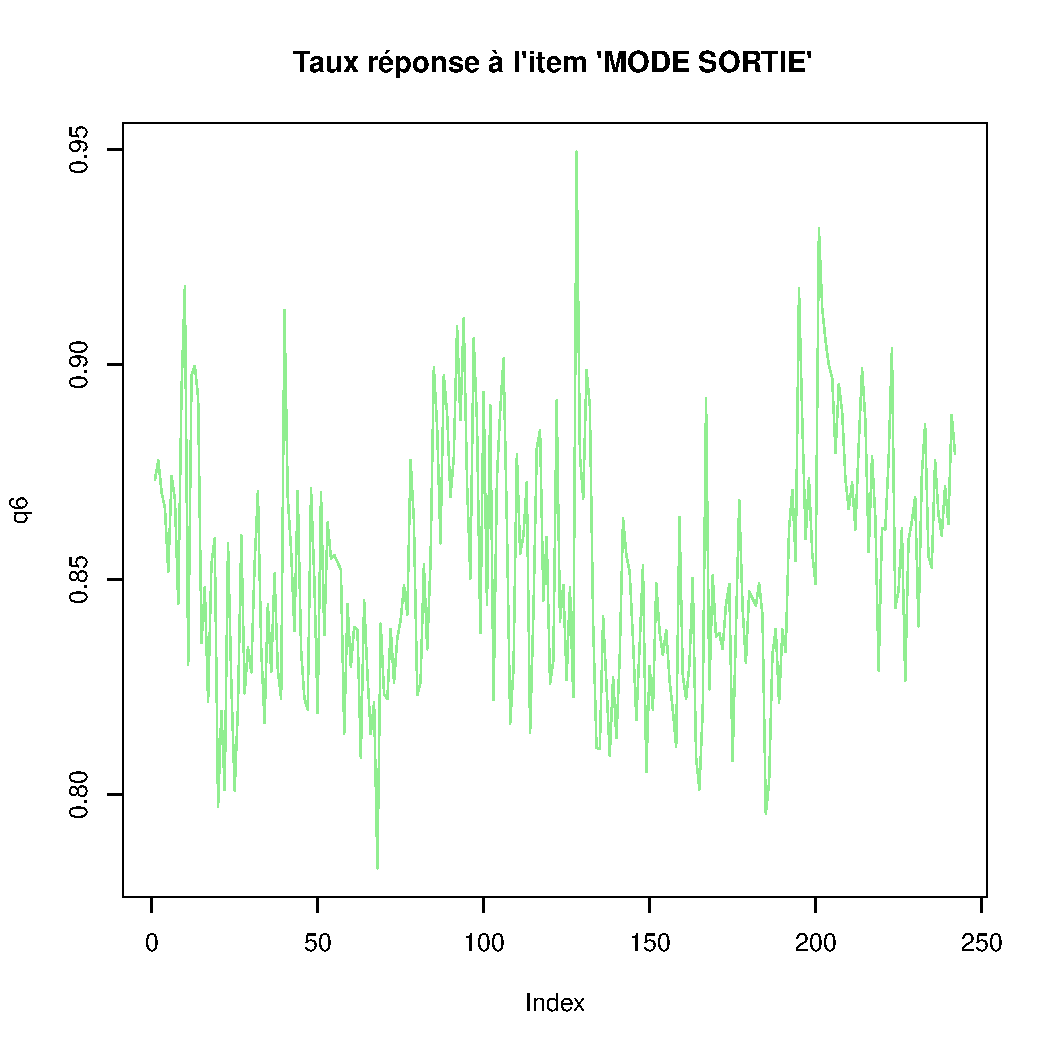
\includegraphics[width=\maxwidth]{figure/retour_dom3} 


\index{exhaustivité@mode de sortie}


%===================================================================== PARTIE 3
\part{Activité par service d'urgence}

\chapter{SAU des Hôpitaux universitaires}

% SuHus.Rnw
% Activité des SU des HUS
Les Hôpitaux universitaires de Strasbourg ont une offre étendue en matière d'urgences et seuleument certaines activités génèrent des RPU.
On compte:
\begin{enumerate}
  \item SU adulte du NHC
  \item SU adulte de HTP
  \item SU pédiatrique de HTP
  \item SU SOS mains (CCOM)
  \item SU Gynéco-obstétrique à HTP
\end{enumerate}
Auxquels il faut rajouter les services assurant un accueil des urgences 24h/24h et qui ne transitent pas par les SU. Ce sont les correspondants privilégiés du SAMU 67 et des transporteurs sanitaires (ASSU, VSAV, SMUR):
\begin{enumerate}
  \item Réanimations médicales de HTP et NHC
  \item Réanimations chirurgicales de HTP et NHC
  \item Réanimation pédiatrique polyvalente de HTP
  \item Unité neuro-vasculaire (HTP)
  \item SI cardio-vasculaire (NHC)
\end{enumerate}

\section{Activité globale}




Entre le 2013-01-01 00:11:00 et le 2013-08-31 23:50:00, \np{25498} RPU ont été transmis, alors que \np{70001} dossiers ont été déclarés au serveur régional. 
1, 1, 1, 1, 1



%===================================================================== PARTIE 4
\part{Activité des SAMU d'Alsace}

\chapter{Test un}

%\SweaveOpts{concordance=TRUE}
\begin{itemize}
  \item test2.Rnw exemple de graphiques avec label
\end{itemize}

\begin{knitrout}
\definecolor{shadecolor}{rgb}{0.969, 0.969, 0.969}\color{fgcolor}\begin{kframe}
\begin{alltt}
n <- \hlkwd{dim}(d1)
\hlkwd{print}(n)
\end{alltt}
\begin{verbatim}
## [1] 222351     20
\end{verbatim}
\begin{alltt}
\hlkwd{names}(d1)
\end{alltt}
\begin{verbatim}
##  [1] "id"            "CODE_POSTAL"   "COMMUNE"       "DESTINATION"  
##  [5] "DP"            "ENTREE"        "EXTRACT"       "FINESS"       
##  [9] "GRAVITE"       "MODE_ENTREE"   "MODE_SORTIE"   "MOTIF"        
## [13] "NAISSANCE"     "ORIENTATION"   "PROVENANCE"    "SEXE"         
## [17] "SORTIE"        "TRANSPORT"     "TRANSPORT_PEC" "AGE"
\end{verbatim}
\end{kframe}
\end{knitrout}



\chapter{test deux}
\begin{knitrout}
\definecolor{shadecolor}{rgb}{0.969, 0.969, 0.969}\color{fgcolor}\begin{kframe}
\begin{alltt}

\hlkwd{str}(d1)
\end{alltt}
\begin{verbatim}
## 'data.frame':	222351 obs. of  20 variables:
##  $ id           : chr  "2c9d83843bf5e01d013bf5e985d20225" "2c9d83843bf5e01d013bf5e986950226" "2c9d83843bf5e01d013bf5e987620227" "2c9d83843bf5e01d013bf5e988060228" ...
##  $ CODE_POSTAL  : Factor w/ 2430 levels "00000","00159",..: 706 706 706 706 706 701 818 706 706 706 ...
##  $ COMMUNE      : Factor w/ 5005 levels "00","01257 DRESDEN ALLEMAGNE",..: 2184 2184 2184 2184 741 2048 2033 2184 2184 2184 ...
##  $ DESTINATION  : Factor w/ 7 levels "NA","MCO","SSR",..: NA NA NA NA NA NA 2 NA 2 NA ...
##  $ DP           : chr  "R104" "J038" "S617" "M485" ...
##  $ ENTREE       : chr  "2013-01-01 00:04:00" "2013-01-01 00:16:00" "2013-01-01 00:26:00" "2013-01-01 00:32:00" ...
##  $ EXTRACT      : chr  "2013-01-01 05:37:00" "2013-01-01 05:37:00" "2013-01-01 05:37:00" "2013-01-01 05:37:00" ...
##  $ FINESS       : Factor w/ 12 levels "3Fr","Alk","Col",..: 10 10 10 10 10 10 10 10 10 10 ...
##  $ GRAVITE      : Factor w/ 7 levels "1","2","3","4",..: 2 2 3 2 2 1 3 2 2 2 ...
##  $ MODE_ENTREE  : Factor w/ 5 levels "NA","Mutation",..: 4 4 4 4 4 4 4 4 4 4 ...
##  $ MODE_SORTIE  : Factor w/ 5 levels "NA","Mutation",..: 4 4 4 4 4 4 2 4 2 4 ...
##  $ MOTIF        : chr  "GASTRO04" "DIVERS23" "TRAUMATO10" "TRAUMATO02" ...
##  $ NAISSANCE    : chr  "1960-04-08 00:00:00" "1986-03-05 00:00:00" "1971-12-22 00:00:00" "1927-04-27 00:00:00" ...
##  $ ORIENTATION  : Factor w/ 13 levels "CHIR","FUGUE",..: NA NA NA NA NA NA 5 NA 5 NA ...
##  $ PROVENANCE   : Factor w/ 7 levels "NA","MCO","SSR",..: 6 6 6 6 6 6 6 6 6 6 ...
##  $ SEXE         : Factor w/ 3 levels "F","I","M": 3 3 3 1 3 3 1 1 1 1 ...
##  $ SORTIE       : chr  "2013-01-01 02:38:00" "2013-01-01 00:38:00" "2013-01-01 02:07:00" "2013-01-01 01:52:00" ...
##  $ TRANSPORT    : Factor w/ 6 levels "AMBU","FO","HELI",..: 4 4 4 1 4 4 6 6 4 4 ...
##  $ TRANSPORT_PEC: Factor w/ 3 levels "AUCUN","MED",..: 1 1 1 3 1 1 2 2 1 1 ...
##  $ AGE          : num  52 26 41 85 39 9 79 50 46 18 ...
\end{verbatim}
\begin{alltt}
\hlkwd{summary}(d1)
\end{alltt}
\begin{verbatim}
##       id             CODE_POSTAL           COMMUNE        DESTINATION    
##  Length:222351      68000  : 15355   MULHOUSE  : 26102   MCO    : 46015  
##  Class :character   68200  : 13754   STRASBOURG: 22812   PSY    :   807  
##  Mode  :character   68100  : 12414   COLMAR    : 15353   SSR    :    56  
##                     67100  : 10377   HAGUENAU  :  4685   HMS    :    18  
##                     67000  :  7349   SELESTAT  :  3845   SLD    :    10  
##                     68500  :  5807   (Other)   :149550   (Other):     1  
##                     (Other):157295   NA's      :     4   NA's   :175444  
##       DP               ENTREE            EXTRACT              FINESS     
##  Length:222351      Length:222351      Length:222351      Col    :44271  
##  Class :character   Class :character   Class :character   Mul    :36619  
##  Mode  :character   Mode  :character   Mode  :character   Hus    :25498  
##                                                           Hag    :23542  
##                                                           Dia    :19699  
##                                                           Sel    :18502  
##                                                           (Other):54220  
##     GRAVITE            MODE_ENTREE        MODE_SORTIE    
##  2      :135883   NA         :     0   NA       :     0  
##  1      : 26301   Mutation   :  2433   Mutation : 43781  
##  3      : 25888   Transfert  :  2255   Transfert:  3204  
##  4      :  2352   Domicile   :193838   Domicile :142443  
##  P      :   943   Transfe  rt:     0   Décès    :     2  
##  (Other):   606   NA's       : 23825   NA's     : 32921  
##  NA's   : 30378                                          
##     MOTIF            NAISSANCE          ORIENTATION       PROVENANCE    
##  Length:222351      Length:222351      UHCD   : 22047   PEA    :122036  
##  Class :character   Class :character   MED    : 11231   PEO    : 19435  
##  Mode  :character   Mode  :character   CHIR   :  4989   MCO    :  5049  
##                                        PSA    :  2058   PSY    :    30  
##                                        REO    :   967   SSR    :    29  
##                                        (Other):  3159   (Other):    15  
##                                        NA's   :177900   NA's   : 75757  
##  SEXE          SORTIE          TRANSPORT      TRANSPORT_PEC   
##  F:105408   Length:222351      AMBU : 30257   AUCUN  :157745  
##  I:     3   Class :character   FO   :   975   MED    :  4520  
##  M:116940   Mode  :character   HELI :   147   PARAMED:  4634  
##                                PERSO:123229   NA's   : 55452  
##                                SMUR :  1860                   
##                                VSAB : 18834                   
##                                NA's : 47049                   
##       AGE       
##  Min.   :  0.0  
##  1st Qu.: 18.0  
##  Median : 38.0  
##  Mean   : 40.6  
##  3rd Qu.: 62.0  
##  Max.   :112.0  
##  NA's   :9
\end{verbatim}
\end{kframe}
\end{knitrout}


\index{test}
\index{Eclipse@Eclipse!solaire}
\index{Orbite!périgée@périgée}
test biblio \cite{1}
%===================================================================== PARTIE 5
\part{Annexes}
\appendix
\chapter{Méthodologie}

% methodologie.Rnw

\section*{Taux de passage aux urgences}
  \begin{displaymath}
    \frac{\text{Nombre de passages déclarés par les SU}}{\text{Population globale d'Alsace}}
  \end{displaymath}

\section*{Taux de recours aux urgences}
\begin{displaymath}
    \frac{\text{Nombre de passages d' Alsace}}{\text{Population globale d'Alsace}}
  \end{displaymath}
Le Nombre de passages d' Alsace est la somme des passages dans les SU alsacien ET des passages de résidents alsacien dans des SU limitrophes.

\section*{Taux d'intervention régional}
\begin{displaymath}
    \frac{\text{Nombre de patients pris en charge par les SMUR d'Alsace}\linebreak[4] \text{ quelque soit le code postal du lieu d'intervention}}{\text{Population globale d'Alsace}}
  \end{displaymath}

\section*{Taux de recours régional}
\begin{displaymath}
    \frac{\text{Nombre de patients pris en charge par un SMUR dont l'intervention a lieu sur le territoire régional }}{\text{Population globale d'Alsace}}
  \end{displaymath}

\section*{Rapport de masculinité ou sex-ratio}
\begin{displaymath}
    \frac{\text{Nombre d'Hommes}}{\text{Nombre de Femmes}} \times 100
\end{displaymath}

Une valeur supérieure à 1 indique qu'il y a plus d'hommes que de femmes.

\section*{Définition de la semaine}
La semaine est définie comme la péride complémentaire du week-end. La semaine s'étend du lundi $08:00$ heures au vendredi $19:59$.

\section*{Définition du Week-end}
L'offre de soins comme la fréquentation des SU n'est pas identique en coiurs de semaine et en fin de semaine. C'est pourquoi est introduite la notion temporelle de week-end.
Le week-end est défini comme la période allant du vendredi soir 20h au lundi matin 07h59.

\section*{Moyenne mobile}
Une moyenne mobile permet de lisser une série de valeurs, permettant de gommer des fluctuations temporelles. La moyenne mobile d'odre $7$ est très utilisée pour analyser les données temporelles. Elle permet notamment d'atténuer les pics de fréquentation des SU le week-end.
\begin{displaymath}
    \frac{\text{somme des passages 7 jours consécutifs}}{7}
\end{displaymath}
Les moyennes mobiles sont généralement présentées sous forme "glissante", c'est à dire sous la forme d'une succession de groupe de sept éléments, décalés d'une journée.

\section*{Pondération annuelle et mensuelle}
Le nombre de jour dans un mois est variable d'un mois à l'autre. Il en va de même pour le nombre de jours d'une année, où du nombre de répétitions d'un jour donné de la semaine.

\chapter{Glossaire}

% glossaire.Rnw

\glossary{AIT Accident (Vasculaire) Ischemique Transitoire}



\subsection*{AIT}
\index{AIT}
Accident (Vasculaire) Ischemique Transitoire

\subsection*{ANTARES}
\index{ANTARES}
Adaptation Nationale des Trasmissions Aux Risques Et Secours

\subsection*{AR}
\index{AR}
Ambulance de Réanimation (voir UMH)

\subsection*{ARS}
\index{ARS}
Agence Régionale de Santé

\subsection*{AVC}
\index{Accident Vasculaire Cérébral}

\subsection*{Population}
\index{Population}

\subsection*{Population comptée à part}
\index{Population@Population!comptée à part}
Le concept de population comptée à part est défini par le décret n°2003-485 publié au Journal officiel du 8 juin 2003, relatif au recensement de la population.
La population comptée à part comprend certaines personnes dont la résidence habituelle (au sens du décret) est dans une autre commune mais qui ont conservé une résidence sur le territoire de la commune :
1. Les mineurs dont la résidence familiale est dans une autre commune mais qui résident, du fait de leurs études, dans la commune.
2. Les personnes ayant une résidence familiale sur le territoire de la commune et résidant dans une communauté d'une autre commune, dès lors que la communauté relève de l'une des catégories suivantes :
- services de moyen ou de long séjour des établissements publics ou privés de santé, établissements sociaux de moyen ou de long séjour, maisons de retraite, foyers et résidences sociales ;
- communautés religieuses ;
- casernes ou établissements militaires.
3. Les personnes majeures âgées de moins de 25 ans ayant leur résidence familiale sur le territoire de la commune et qui résident dans une autre commune pour leurs études.
4. Les personnes sans domicile fixe rattachées à la commune au sens de la loi du 3 janvier 1969 et non recensées dans la commune. \cite{8}


\subsection*{Population totale}
\index{Population@Population!totale}r
Le concept de *population totale* est défini par le décret n°2003-485 publié au Journal officiel du 8 juin 2003, relatif au recensement de la population.

La population totale d'une commune est égale à la somme de la population municipale et de la population comptée à part de la commune.
La population totale d'un ensemble de communes est égale à la somme des populations totales des communes qui le composent.
La population totale est une population légale à laquelle de très nombreux textes législatifs ou réglementaires font référence. A la différence de la population municipale, elle n'a pas d'utilisation statistique car elle comprend des doubles comptes dès lors que l'on s'intéresse à un ensemble de plusieurs communes \cite{7}.

\subsection*{Population municipale}
\index{Population@Population!municipale}
Le concept de *population municipale* est défini par le décret n°2003-485 publié au Journal officiel du 8 juin 2003, relatif au recensement de la population.
La population municipale comprend les personnes ayant leur résidence habituelle (au sens du décret) sur le territoire de la commune, dans un logement ou une communauté, les personnes détenues dans les établissements pénitentiaires de la commune, les personnes sans-abri recensées sur le territoire de la commune et les personnes résidant habituellement dans une habitation mobile recensée sur le territoire de la commune.
La population municipale d'un ensemble de communes est égale à la somme des populations municipales des communes qui le composent.
Le concept de \emph{population municipale} correspond désormais à la notion de \emph{population utilisée usuellement en statistique}. En effet, elle ne comporte pas de doubles comptes : chaque personne vivant en France est comptée une fois et une seule. En 1999, c'était le concept de population sans doubles comptes qui correspondait à la notion de population statistique \cite{6}.


\subsection*{Unité urbaine}
\index{Unité urbaine}
La notion d'unité urbaine repose sur la continuité du bâti et le nombre d'habitants. On appelle unité urbaine une commune ou un ensemble de communes présentant une zone de bâti continu (pas de coupure de plus de 200 mètres entre deux constructions) qui compte au moins 2 000 habitants.
Si l'unité urbaine se situe sur une seule commune, elle est dénommée ville isolée. Si l'unité urbaine s'étend sur plusieurs communes, et si chacune de ces communes concentre plus de la moitié de sa population dans la zone de bâti continu, elle est dénommée agglomération multicommunale.
Sont considérées comme rurales les communes qui ne rentrent pas dans la constitution d'une unité urbaine : les communes sans zone de bâti continu de 2000 habitants, et celles dont moins de la moitié de la population municipale est dans une zone de bâti continu (INSEE \cite{4}).

cellule régionale d’appui et de pilotage sanitaire (CRAPS)
service zonal de défense et de sécurité (SZDS)
plateforme de veille et d’urgence sanitaire (PVUS)
cellule zonale d’appui (CZA). Structure de crise de l’ARS de zone, elle est constituée autour du SZDS qui assure une fonction de coordination en collaboration étroite avec la/les CRAPS activée(s) en ARS.
Directeur général de la santé (DGS) ou le Haut fonctionnaire de défense et de sécurité (HFDS)
Centre de crise sanitaire (CCS
Centre opérationnel zonal renforcé (COZ-R) de l’état-major interministériel de zone de défense et de sécurité (EMIZDS).
Système d’information sanitaire des alertes et crises (SISAC) de la DGS.




\chapter{RPU}
\chapter{A propos de ce document}

% apropos.Rnw

Ce document a été totalement rédigé à l'aide du logiciel R \cite{5} en respectant les recommandations de la \emph{Reproducible Research}. Le but de la recherche reproductible consiste à lier les données expérimentales et leur analyse par des instructions spécifiques de sorte que les résultats peuvent être reproduits, mieux compris et vérifiés.

\chapter{Bibliographie}
\bibliography{../../rpu}
\chapter{Index}
\printindex
\end{document}
